% !TeX spellcheck = de-DE
% !TeX encoding = utf8
% !TeX program = pdflatex
% !BIB program = biber
% -*- coding:utf-8 mod:LaTeX -*-

% vv  scroll down to line 200 for content  vv


\let\ifdeutsch\iftrue
\let\ifenglisch\iffalse
\input{pre-documentclass}
\documentclass[
  ngerman,
  % fontsize=11pt is the standard
  a4paper,  % Standard format - only KOMAScript uses paper=a4 - https://tex.stackexchange.com/a/61044/9075
  twoside,  % we are optimizing for both screen and two-sided printing. So the page numbers will jump, but the content is configured to stay in the middle (by using the geometry package)
  bibliography=totoc,
  %               idxtotoc,   %Index ins Inhaltsverzeichnis
  %               liststotoc, %List of X ins Inhaltsverzeichnis, mit liststotocnumbered werden die Abbildungsverzeichnisse nummeriert
  headsepline,
  cleardoublepage=empty,
  parskip=half,
  %               draft    % um zu sehen, wo noch nachgebessert werden muss - wichtig, da Bindungskorrektur mit drin
  draft=false
]{scrbook}
% !TeX encoding = utf8
% -*- coding:utf-8 mod:LaTeX -*-

% EN: This file includes basic packages and sets options. The order of package
%     loading is important

% DE: In dieser Datei werden zuerst die benoetigten Pakete eingebunden und
%     danach diverse Optionen gesetzt. Achtung Reihenfolge ist entscheidend!


% EN: Styleguide:
% - English comments are prefixed with "EN", German comments are prefixed with "DE"
% - Prefixed headings define the language for the subsequent paragraphs
% - It is tried to organize packages in blocks. Bocks are separated by two empty lines.

% DE: Styleguide:
%
% Ein sehr kleiner Styleguide. Packages werden in Blöcken organisiert.
% Zwischen zwei Blöcken sind 2 Leerzeilen!


% EN: Enable copy and paste of text from the PDF
%     Only required for pdflatex. It "just works" in the case of lualatex.
%     mmap enables mathematical symbols but does not work with the newtx font set
%     See: https://tex.stackexchange.com/a/64457/9075
%     Other solutions outlined at http://goemonx.blogspot.de/2012/01/pdflatex-ligaturen-und-copynpaste.html and http://tex.stackexchange.com/questions/4397/make-ligatures-in-linux-libertine-copyable-and-searchable
%     Troubleshooting outlined at https://tex.stackexchange.com/a/100618/9075

\ifluatex
\else
  \usepackage{cmap}
\fi


% EN: File encoding
% DE: Codierung
%     Wir sind im 21 Jahrhundert, utf-8 löst so viele Probleme.
%
% Mit UTF-8 funktionieren folgende Pakete nicht mehr. Bitte beachten!
%   * fancyvrb mit §
%   * easylist -> http://www.ctan.org/tex-archive/macros/latex/contrib/easylist/
\ifluatex
  % EN: See https://tex.stackexchange.com/a/158517/9075
  %     Not required, because of usage of fontspec package
  %\usepackage[utf8]{luainputenc}
\else
  \usepackage[utf8]{inputenc}
\fi


% DE: Parallelbetrieb tex4ht und pdflatex

\makeatletter
\@ifpackageloaded{tex4ht}{
  \def\iftex4ht{\iftrue}
}{
  \def\iftex4ht{\iffalse}
}
\makeatother


% EN: Mathematics
% DE: Mathematik
%
% DE: Viele Mathematik-Sachen. Siehe https://texdoc.net/pkg/amsmath
%
% EN: Options must be passed this way, otherwise it does not work with glossaries
% DE: fleqn (=Gleichungen linksbündig platzieren) funktioniert nicht direkt. Es muss noch ein Patch gemacht werden:
\PassOptionsToPackage{fleqn,leqno}{amsmath}
%
% DE: amsmath Muss nicht mehr geladen werden, da es von newtxmath automatisch geladen wird
% \usepackage{amsmath}


%% EN: Fonts
%% DE: Schriften
%%
%% !!! If you change the font, be sure that words such as "workflow" can
%% !!! still be copied from the PDF. If this is not the case, you have
%% !!! to use glyphtounicode. See comment at cmap package


% EN: Times Roman for all text
\ifluatex
  \RequirePackage{amsmath}
  \RequirePackage{unicode-math}
  \setmainfont{TeX Gyre Termes}
  \setmathfont{texgyretermes-math.otf}
  \setsansfont[Scale=.9]{TeX Gyre Heros}
  \setmonofont[StylisticSet={1,3},Scale=.9]{inconsolata}
\else
  \RequirePackage{newtxtext}
  \RequirePackage{newtxmath}
  % EN: looks good with times, but no equivalent for lualatex found,
  %     therefore replaced with inconsolata
  %\RequirePackage[zerostyle=b,scaled=.9]{newtxtt}
  \RequirePackage[varl,scaled=.9]{inconsolata}

  % DE: Symbole
  % unicode-math scheint für die meisten schon etwas anzubieten
  %
  %\usepackage[geometry]{ifsym} % \BigSquare

  % EN: The euro sign
  % DE: Das Euro Zeichen
  %     Fuer Palatino (mathpazo.sty): richtiges Euro-Zeichen
  %     Alternative: \usepackage{eurosym}
  \newcommand{\EUR}{\ppleuro}
\fi


% DE: Noch mehr Symbole
%\usepackage{stmaryrd} %fuer \ovee, \owedge, \otimes
%\usepackage{marvosym} %fuer \Writinghand %patched to not redefine \Rightarrow
%\usepackage{mathrsfs} %mittels \mathscr{} schoenen geschwungenen Buchstaben erzeugen
%\usepackage{calrsfs} %\mathcal{} ein bisserl dickeren buchstaben erzeugen - sieht net so gut aus.

% EN: Fallback font - if the subsequent font packages do not define a font (e.g., monospaced)
%     This is the modern package for "Computer Modern".
%     In case this gets activated, one has to switch from cmap package to glyphtounicode (in the case of pdflatex)
% DE: Fallback-Schriftart
%\usepackage[%
%    rm={oldstyle=false,proportional=true},%
%    sf={oldstyle=false,proportional=true},%
%    tt={oldstyle=false,proportional=true,variable=true},%
%    qt=false%
%]{cfr-lm}

% EN: Headings are typset in Helvetica (which is similar to Arial)
% DE: Schriftart fuer die Ueberschriften - ueberschreibt lmodern
%\usepackage[scaled=.95]{helvet}

% DE: Für Schreibschrift würde tun, muss aber nicht
%\usepackage{mathrsfs} %  \mathscr{ABC}

% EN: Font for the main text
% DE: Schriftart fuer den Fliesstext - ueberschreibt lmodern
%     Linux Libertine, siehe http://www.linuxlibertine.org/
%     Packageparamter [osf] = Minuskel-Ziffern
%     rm = libertine im Brottext, Linux Biolinum NICHT als serifenlose Schrift, sondern helvet (von oben) beibehalten
%\usepackage[rm]{libertine}

% EN: Alternative Font: Palantino. It is recommended by Prof. Ludewig for German texts
% DE: Alternative Schriftart: Palantino, Packageparamter [osf] = Minuskel-Ziffern
%     Bitte nur in deutschen Texten
%\usepackage{mathpazo} %ftp://ftp.dante.de/tex-archive/fonts/mathpazo/ - Tipp aus DE-TEX-FAQ 8.2.1

% DE: Schriftart fuer Programmcode - ueberschreibt lmodern
%     Falls auskommentiert, wird die Standardschriftart lmodern genommen
%     Fuer schreibmaschinenartige Schluesselwoerter in den Listings - geht bei alten Installationen nicht, da einige Fontshapes (<>=) fehlen
%\usepackage[scaled=.92]{luximono}
%\usepackage{courier}
% DE: BeraMono als Typewriter-Schrift, Tipp von http://tex.stackexchange.com/a/71346/9075
%\usepackage[scaled=0.83]{beramono}

% EN: backticks (`) are rendered as such in verbatim environments.
%     See the following links for details:
%     - https://tex.stackexchange.com/a/341057/9075
%     - https://tex.stackexchange.com/a/47451/9075
%     - https://tex.stackexchange.com/a/166791/9075
\usepackage{upquote}

% EN: For \texttrademark{}
\usepackage{textcomp}

% EN: name-clashes von marvosym und mathabx vermeiden:
\def\delsym#1{%
  %  \expandafter\let\expandafter\origsym\expandafter=\csname#1\endcsname
  %  \expandafter\let\csname orig#1\endcsname=\origsym
  \expandafter\let\csname#1\endcsname=\relax
}

%\usepackage{pifont}
%\usepackage{bbding}
%\delsym{Asterisk}
%\delsym{Sun}\delsym{Mercury}\delsym{Venus}\delsym{Earth}\delsym{Mars}
%\delsym{Jupiter}\delsym{Saturn}\delsym{Uranus}\delsym{Neptune}
%\delsym{Pluto}\delsym{Aries}\delsym{Taurus}\delsym{Gemini}
%\delsym{Rightarrow}
%\usepackage{mathabx} - Ueberschreibt leider zu viel - und die \le-Zeichen usw. sehen nicht gut aus!


% EN: Modern font encoding
%     Has to be loaded AFTER any font packages. See https://tex.stackexchange.com/a/2869/9075.
\ifluatex
\else
  \usepackage[T1]{fontenc}
\fi
%


% EN: Character protrusion and font expansion. See http://www.ctan.org/tex-archive/macros/latex/contrib/microtype/
% DE: Optischer Randausgleich und Grauwertkorrektur

\usepackage[
  babel=true, % EN: Enable language-specific kerning. Take language-settings from the language of the current document (see Section 6 of microtype.pdf)
  expansion=alltext,
  protrusion=alltext-nott, % EN: Ensure that at listings, there is no change at the margin of the listing
  final % EN: Always enable microtype, even if in draft mode. This helps finding bad boxes quickly.
        %     In the standard configuration, this template is always in the final mode, so this option only makes a difference if "pros" use the draft mode
]{microtype}


% EN: \texttt{test -- test} keeps the "--" as "--" (and does not convert it to an en dash)
\DisableLigatures{encoding = T1, family = tt* }

% DE: fuer microtype
% DE: tracking=true muss als Parameter des microtype-packages mitgegeben werden
% DE: Deaktiviert, da dies bei Algorithmen seltsam aussieht

%\DeclareMicrotypeSet*[tracking]{my}{ font = */*/*/sc/* }%
%\SetTracking{ encoding = *, shape = sc }{ 45 }
% DE: Hier wird festgelegt,
%     dass alle Passagen in Kapitälchen automatisch leicht
%     gesperrt werden.
%     Quelle: http://homepage.ruhr-uni-bochum.de/Georg.Verweyen/pakete.html
%    Deaktiviert, da sonst "BPEL", "BPMN" usw. wirklich komisch aussehen.
%     Macht wohl nur bei geisteswissenschaftlichen Arbeiten Sinn.


% EN: amsmath teaks


% EN: Fixes bugs in AMS math
%     Currently conflicts with unicode-math
% \usepackage{mathtools}

%\numberwithin{equation}{section}
%\renewcommand{\theequation}{\thesection.\Roman{equation}}

% EN: work-around ams-math problem with align and 9 -> 10. Does not work with glossaries, No visual changes.
%\addtolength\mathindent{1em}


% EN: For theorems, replacement for amsthm
\usepackage[amsmath,hyperref]{ntheorem}
\theorempreskipamount 2ex plus1ex minus0.5ex
\theorempostskipamount 2ex plus1ex minus0.5ex
\theoremstyle{break}
\newtheorem{definition}{Definition}[section]


% CTAN: https://ctan.org/pkg/lccaps
% Doc: http://texdoc.net/pkg/lccaps
%
% Required for DE/EN \initialism
\usepackage{lccaps}


% EN: Definition of colors. The "hyperref" argument is not used as we do not want to change the border colors of links: Links are not colored anymore.
% DE: Farbdefinitionen
\usepackage[dvipsnames]{xcolor}


% EN: Required for custom acronyms/glossaries style.
%     Left aligned Columns in tables with fixed width.
%     See http://tex.stackexchange.com/questions/91566/syntax-similar-to-centering-for-right-and-left
\usepackage{ragged2e}


% DE: Wichtig, ansonsten erscheint "No room for a new \write"
\usepackage{scrwfile}


% EN: Support for language-specific hyphenation
% DE: Neue deutsche Rechtschreibung und Literatur statt "Literature"
%     Die folgende Einstellung ist der Nachfolger von ngerman.sty
\ifdeutsch
  % DE: letzte Sprache ist default, Einbindung von "american" ermöglicht \begin{otherlanguage}{amercian}...\end{otherlanguage} oder \foreignlanguage{american}{Text in American}
  %     Siehe auch http://tex.stackexchange.com/a/50638/9075
  \usepackage[american,main=ngerman]{babel}
  % Ein "abstract" ist eine "Kurzfassung", keine "Zusammenfassung"
  \addto\captionsngerman{%
    \renewcommand\abstractname{Kurzfassung}%
  }
  \ifluatex
    % EN: conditionally disable ligatures. See https://github.com/latextemplates/scientific-thesis-template/issues/54
    %     for a discussion
    \usepackage[ngerman]{selnolig}
  \fi
\else
  % EN: Set English as the language and allow to write hyphenated"=words
  %     `american`, `english` and `USenglish` are synonyms for babel package (according to https://tex.stackexchange.com/questions/12775/babel-english-american-usenglish).
  %      "english" has to go last to set it as the default language
  \usepackage[ngerman,main=english]{babel}
  % EN: Hint by http://tex.stackexchange.com/a/321066/9075 -> enable "= as dashes
  \addto\extrasenglish{\languageshorthands{ngerman}\useshorthands{"}}
  \ifluatex
    % EN: conditionally disable ligatures. See https://github.com/latextemplates/scientific-thesis-template/issues/54
    %     for a discussion
    \usepackage[english]{selnolig}
  \fi
\fi
%


% EN: For easy quotations: \enquote{text}
%     This package is very smart when nesting is applied, otherwise textcmds (see below) provides a shorter command
%     Note that this package results in a warning when it is loaded before minted (actually fvextra).
% DE: Anführungszeichen
%     Zitate in \enquote{...} setzen, dann werden automatisch die richtigen Anführungszeichen verwendet.
%     Dieses package erzeugt eine Warnung, wenn es vor minted (genauer fvextra) geladen wird.
\usepackage{csquotes}


% EN: For even easier quotations: \qq{text}.
%     Is not smart in the case of nesting, but good enough for most cases
\usepackage{textcmds}
\ifdeutsch
  % EN: German quotes are different. So do not use the English quotes, but the ones provided by the csquotes package.
  \renewcommand{\qq}[1]{\enquote{#1}}
\fi


% EN: extended enumarations
% DE: erweitertes Enumerate
\usepackage{paralist}


% DE: Gestaltung der Kopf- und Fußteilen

\usepackage[automark]{scrlayer-scrpage}

\automark[section]{chapter}
\setkomafont{pageheadfoot}{\normalfont\sffamily}
\setkomafont{pagenumber}{\normalfont\sffamily}

% DE: funktioniert nicht: Alle Linien sind hier weg
%\setheadsepline[.4pt]{.4pt}


% DE: Intelligentes Leerzeichen um hinter Abkürzungen die richtigen Abstände zu erhalten, auch leere.
%     Siehe commands.tex \gq{}
\usepackage{xspace}
% DE: Macht \xspace und \enquote kompatibel
\makeatletter
\xspaceaddexceptions{\grqq \grq \csq@qclose@i \} }
\makeatother


\newcommand{\eg}{e.\,g.,\ }
\newcommand{\ie}{i.\,e.,\ }


% EN: introduce \powerset - hint by http://matheplanet.com/matheplanet/nuke/html/viewtopic.php?topic=136492&post_id=997377
\DeclareFontFamily{U}{MnSymbolC}{}
\DeclareSymbolFont{MnSyC}{U}{MnSymbolC}{m}{n}
\DeclareFontShape{U}{MnSymbolC}{m}{n}{
  <-6>    MnSymbolC5
  <6-7>   MnSymbolC6
  <7-8>   MnSymbolC7
  <8-9>   MnSymbolC8
  <9-10>  MnSymbolC9
  <10-12> MnSymbolC10
  <12->   MnSymbolC12%
}{}
\DeclareMathSymbol{\powerset}{\mathord}{MnSyC}{180}


% EN: Package for the appendix
% DE: Anhang
\usepackage{appendix}
%[toc,page,title,header]
%


% EN: Graphics
% DE: Grafikeinbindungen
%
% EN: The parameter "pdftex" is not required
\usepackage{graphicx}
\graphicspath{{\getgraphicspath}}
\newcommand{\getgraphicspath}{graphics/}


% EN: Enables inclusion of SVG graphics - 1:1 approach
%    This is NOT the approach of https://ctan.org/pkg/svg-inkscape,
%     which allows text in SVG to be typeset using LaTeX
%     We just include the SVG as is.
\usepackage{epstopdf}
\epstopdfDeclareGraphicsRule{.svg}{pdf}{.pdf}{%
  inkscape -z -D --file=#1 --export-pdf=\OutputFile
}


% EN: Enables inclusion of SVG graphics - text-rendered-with-LaTeX-approach
%     This is the approach of https://ctan.org/pkg/svg-inkscape,
\newcommand{\executeiffilenewer}[3]{%
  \IfFileExists{#2}
  {
    %\message{file #2 exists}
    \ifnum\pdfstrcmp{\pdffilemoddate{#1}}%
      {\pdffilemoddate{#2}}>0%
      {\immediate\write18{#3}}
    \else
      {%\message{file up to date #2}
      }
    \fi%
  }{
    %\message{file #2 doesn't exist}
    %\message{argument: #3}
    %\immediate\write18{echo "test" > xoutput.txt}
    \immediate\write18{#3}
  }
}
\newcommand{\includesvg}[1]{%
  \executeiffilenewer{#1.svg}{#1.pdf}%
  {
    inkscape -z -D --file=\getgraphicspath#1.svg %
    --export-pdf=\getgraphicspath#1.pdf --export-latex}%
  \input{\getgraphicspath#1.pdf_tex}%
}


% EN: Enable typesetting values with SI units.
\ifdeutsch
  \usepackage[mode=text,group-minimum-digits=4]{siunitx}
  \sisetup{locale=DE}
\else
  \usepackage[mode=text,group-minimum-digits=4,group-separator={,}]{siunitx}
  \sisetup{locale=US}
\fi


% EN: Extensions for tables
% DE: Tabellenerweiterungen
\usepackage{array} %increases tex's buffer size and enables ``>'' in tablespecs
\usepackage{longtable}
\usepackage{dcolumn} %Aligning numbers by decimal points in table columns
\ifdeutsch
  \newcolumntype{d}[1]{D{.}{,}{#1}}
\else
  \newcolumntype{d}[1]{D{.}{.}{#1}}
\fi
\setlength{\extrarowheight}{1pt}


% DE: Eine Zelle, die sich über mehrere Zeilen erstreckt.
%     Siehe Beispieltabelle in Kapitel 2
\usepackage{multirow}


% DE: Fuer Tabellen mit Variablen Spaltenbreiten
%\usepackage{tabularx}
%\usepackage{tabulary}


% EN: Links behave as they should. Enables "\url{...}" for URL typesettings.
%     Allow URL breaks also at a hyphen, even though it might be confusing: Is the "-" part of the address or just a hyphen?
%     See https://tex.stackexchange.com/a/3034/9075.
% DE: Links verhalten sich so, wie sie sollen
%     Zeilenumbrüche bei URLs auch bei Bindestrichen erlauben, auch wenn es verwirrend sein könnte: Gehört der Bindestrich zur URL oder ist es ein Trennstrich?
%     Siehe https://tex.stackexchange.com/a/3034/9075.
\usepackage[hyphens]{url}
%
%  EN: When activated, use text font as URL font, not the monospaced one.
%      For all options see https://tex.stackexchange.com/a/261435/9075.
% \urlstyle{same}
%
% EN: Hint by http://tex.stackexchange.com/a/10419/9075.
\makeatletter
\g@addto@macro{\UrlBreaks}{\UrlOrds}
\makeatother


% DE: Index über Begriffe, Abkürzungen
%\usepackage{makeidx} makeidx ist out -> http://xindy.sf.net verwenden


% DE: lustiger Hack fuer das Abkuerzungsverzeichnis
%     nach latex durchlauf folgendes ausfuehren
%     makeindex ausarbeitung.nlo -s nomencl.ist -o ausarbeitung.nls
%     danach nochmal latex
%\usepackage{nomencl}
%    \let\abk\nomenclature %Deutsche Ueberschrift setzen
%          \renewcommand{\nomname}{List of Abbreviations}
%        %Punkte zw. Abkuerzung und Erklaerung
%          \setlength{\nomlabelwidth}{.2\hsize}
%          \renewcommand{\nomlabel}[1]{#1 \dotfill}
%        %Zeilenabstaende verkleinern
%          \setlength{\nomitemsep}{-\parsep}
%    \makenomenclature


% EN: Logic for TeX - enables if-then-else in commands
% DE: Logik für TeX
%     FÜr if-then-else @ commands.tex
\usepackage{ifthen}


% EN: Code Listings
% DE: Listings
\usepackage{listings}
\lstset{language=XML,
  showstringspaces=false,
  extendedchars=true,
  basicstyle=\footnotesize\ttfamily,
  commentstyle=\slshape,
  % DE: Original: \rmfamily, damit werden die Strings im Quellcode hervorgehoben. Zusaetzlich evtl.: \scshape oder \rmfamily durch \ttfamily ersetzen. Dann sieht's aus, wie bei fancyvrb
  stringstyle=\ttfamily,
  breaklines=true,
  breakatwhitespace=true,
  % EN: alternative: fixed
  columns=flexible,
  numbers=left,
  numberstyle=\tiny,
  basewidth=.5em,
  xleftmargin=.5cm,
  % aboveskip=0mm, %DE: deaktivieren, falls man lstlistings direkt als floating object benutzt (\begin{lstlisting}[float,...])
  % belowskip=0mm, %DE: deaktivieren, falls man lstlistings direkt als floating object benutzt (\begin{lstlisting}[float,...])
  captionpos=b
}
\lstdefinelanguage{Excel}{
    keywords={IF, SUM, AVERAGE, COUNT, AND, OR, NOT},
    morekeywords={=},
    sensitive=false,
    alsoletter={=},
    morecomment=[l]{'},
    morestring=[b]",
    columns=fullflexible,
}

\lstset{
    language=Excel,
    basicstyle=\ttfamily\small, % Schriftgröße und -art
    keywordstyle=\color{blue},  % Farbe für Schlüsselwörter
    commentstyle=\color{green!60!black}, % Farbe für Kommentare
    stringstyle=\color{red}, % Farbe für Zeichenketten
    showstringspaces=false,
    breaklines=false, % Zeilen umbrechen
    breakatwhitespace=true,
    frame=single, % Rahmen um den Code
    tabsize=4, % Tabulatorgröße
    captionpos=b % Position der Caption
    breakindent=2em,
}

\ifluatex
\else
  % EN: Enable UTF-8 support - see https://tex.stackexchange.com/q/419327/9075
  \usepackage{listingsutf8}
  \lstset{inputencoding=utf8/latin1}
\fi

\ifdeutsch
  \renewcommand{\lstlistlistingname}{Verzeichnis der Listings}
\fi


% EN: Alternative to listings could be fancyvrb. Can be used together.
% DE: Alternative zu Listings ist fancyvrb. Kann auch beides gleichzeitig benutzt werden.
\usepackage{fancyvrb}
%
% EN: Font size for the normal text
% DE: Groesse fuer den Fliesstext. Falls deaktiviert: \normalsize
%\fvset{fontsize=\small}
%
% DE: Somit kann im Text ganz einfach §verbatim§ text gesetzt werden.
%     Disabled, because UTF-8 does not work any more and lualatex causes issues
%\DefineShortVerb{\§}
%
% EN: Shrink font size of listings
\RecustomVerbatimEnvironment{Verbatim}{Verbatim}{fontsize=\footnotesize}
\RecustomVerbatimCommand{\VerbatimInput}{VerbatimInput}{fontsize=\footnotesize}
%
% EN: Hack for fancyvrb based on http://newsgroups.derkeiler.com/Archive/Comp/comp.text.tex/2008-12/msg00075.html
%     Change of the solution: \Vref somehow collided with cleveref/varioref as the output of \Vref{} was "Abschnitt 4.3 auf Seite 85"; therefore changed to \myVref -- so completely removed
%     See https://tex.stackexchange.com/q/132420/9075 for more information.
\newcommand{\Vlabel}[1]{\label[line]{#1}\hypertarget{#1}{}}
\newcommand{\lref}[1]{\hyperlink{#1}{\FancyVerbLineautorefname~\ref*{#1}}}


% EN: Tunings of captions for floats, listings, ...
% DE: Bildunterschriften bei floats genauso formatieren wie bei Listings
%     Anpassung wird unten bei den newfloat-Deklarationen vorgenommen
%     https://www.ctan.org/pkg/caption2 is superseeded by this package.
\usepackage{caption}


% EN: Provides rotating figures, where the PDF page is also turned
% DE: Ermoeglicht es, Abbildungen um 90 Grad zu drehen
%     Alternatives Paket: rotating Allerdings wird hier nur das Bild gedreht, während bei lscape auch die PDF-Seite gedreht wird.
%     Das Paket lscape dreht die Seite auch nicht
\usepackage{pdflscape}


% EN: Required for proper environments of fancyvrb and lstlistings
%    There is also the newfloat package (recommended by minted), but we currently have no experience with that
% DE: Wird für fancyvrb und für lstlistings verwendet
\usepackage{float}
%
% EN: Alternative to float package
%\usepackage{floatrow}
% DE: zustäzlich für den Paramter [H] = Floats WIRKLICH da wo sie deklariert wurden paltzieren - ganz ohne Kompromisse
%     floatrow ist der Nachfolger von float
%     Allerdings macht floatrow in manchen Konstellationen Probleme. Deshalb ist das Paket deaktiviert.
%
% EN: See http://www.tex.ac.uk/cgi-bin/texfaq2html?label=floats
% DE: floats IMMER nach einer Referenzierung platzieren
%\usepackage{flafter}


% EN: Put footnotes below floats
%     Source: https://tex.stackexchange.com/a/32993/9075
\usepackage{stfloats}
\fnbelowfloat


% EN: For nested figures
% DE: Fuer Abbildungen innerhalb von Abbildungen
%     Ersetzt die Pakete subfigure und subfig - siehe https://tex.stackexchange.com/a/13778/9075
\usepackage[hypcap=true]{subcaption}


% EN: Extended support for footnotes
% DE: Fußnoten
%
%\usepackage{dblfnote}  %Zweispaltige Fußnoten
%
% Keine hochgestellten Ziffern in der Fußnote (KOMA-Script-spezifisch):
%\deffootnote[1.5em]{0pt}{1em}{\makebox[1.5em][l]{\bfseries\thefootnotemark}}
%
% Abstand zwischen Fußnoten vergrößern:
%\setlength{\footnotesep}{.85\baselineskip}
%
% EN: Following command disables the separating line of the footnote
% DE: Folgendes Kommando deaktiviert die Trennlinie zur Fußnote
%\renewcommand{\footnoterule}{}
%
\addtolength{\skip\footins}{\baselineskip} % Abstand Text <-> Fußnote
%
% Fußnoten immer ganz unten auf einer \raggedbottom-Seite
% fnpos kommt aus dem yafoot package
\usepackage{fnpos}
\makeFNbelow
\makeFNbottom


% EN: Variable page heights
% DE: Variable Seitenhöhen zulassen
\raggedbottom


% DE: Falls die Seitenzahl bei einer Referenz auf eine Abbildung nur dann angegeben werden soll,
%     falls sich die Abbildung nicht auf der selben Seite befindet...
\iftex4ht
  %tex4ht does not work well with vref, therefore we emulate vref behavior
  \newcommand{\vref}[1]{\ref{#1}}
\else
  \ifdeutsch
    \usepackage[ngerman]{varioref}
  \else
    \usepackage{varioref}
  \fi
\fi


% EN: More beautiful tables if one uses \toprule, \midrule, \bottomrule
% DE: Noch schoenere Tabellen als mit booktabs mit http://www.zvisionwelt.de/downloads.html
\usepackage{booktabs}
%
%\usepackage[section]{placeins}


% EN: Graphs and Automata
%
% TODO: Since version 3.0 (2013-10-01), it supports pdflatex via the auto-pst-pdf package
%       Requires -shell-escape
%\usepackage{gastex}


%\usepackage{multicol}

% DE: kollidiert mit diplomarbeit.sty
%\usepackage{setspace}


% DE: biblatex statt bibtex
\usepackage[
  backend       = biber, %biber does not work with 64x versions alternative: bibtex8
  %minalphanames only works with biber backend
  sortcites     = true,
  bibstyle      = alphabetic,
  citestyle     = alphabetic,
  giveninits    = true,
  useprefix     = false, %"von, van, etc." will be printed, too. See below.
  minnames      = 1,
  minalphanames = 3,
  maxalphanames = 4,
  maxbibnames   = 99,
  maxcitenames  = 2,
  natbib        = true,
  eprint        = true,
  url           = true,
  doi           = true,
  isbn          = true,
  backref       = true]{biblatex}

% enable more breaks at URLs. See https://tex.stackexchange.com/a/134281.
\setcounter{biburllcpenalty}{7000}
\setcounter{biburlucpenalty}{8000}

\bibliography{bibliography}
%\addbibresource[datatype=bibtex]{bibliography.bib}

%Do not put "vd" in the label, but put it at "\citeauthor"
%Source: http://tex.stackexchange.com/a/30277/9075
\makeatletter
\AtBeginDocument{\toggletrue{blx@useprefix}}
\AtBeginBibliography{\togglefalse{blx@useprefix}}
\makeatother

%Thin spaces between initials
%http://tex.stackexchange.com/a/11083/9075
\renewrobustcmd*{\bibinitdelim}{\,}

%Keep first and last name together in the bibliography
%http://tex.stackexchange.com/a/196192/9075
\renewcommand*\bibnamedelimc{\addnbspace}
\renewcommand*\bibnamedelimd{\addnbspace}

%Replace last "and" with a comma in bibliography
%See http://tex.stackexchange.com/a/41532/9075
\AtBeginBibliography{%
  \renewcommand*{\finalnamedelim}{\addcomma\space}%
}

\DefineBibliographyStrings{ngerman}{
  backrefpage  = {zitiert auf S\adddot},
  backrefpages = {zitiert auf S\adddot},
  andothers    = {et\ \addabbrvspace al\adddot},
  %Tipp von http://www.mrunix.de/forums/showthread.php?64665-biblatex-Kann-%DCberschrift-vom-Inhaltsverzeichnis-nicht-%E4ndern&p=293656&viewfull=1#post293656
  bibliography = {Literaturverzeichnis}
}

% EN: enable hyperlinked author names when using~\citeauthor
%     source: http://tex.stackexchange.com/a/75916/9075
\DeclareCiteCommand{\citeauthor}
{\boolfalse{citetracker}%
  \boolfalse{pagetracker}%
  \usebibmacro{prenote}}
{\ifciteindex
  {\indexnames{labelname}}
  {}%
  \printtext[bibhyperref]{\printnames{labelname}}}
{\multicitedelim}
{\usebibmacro{postnote}}

% EN: natbib compatibility
%\newcommand{\citep}[1]{\cite{#1}}
%\newcommand{\citet}[1]{\citeauthor{#1}~\cite{#1}}
% EN: Beginning of sentence - analogous to cleveref - important for names such as "zur Muehlen"
%\newcommand{\Citep}[1]{\cite{#1}}
%\newcommand{\Citet}[1]{\Citeauthor{#1}~\cite{#1}}

% DE: Blindtext. Paket "blindtext" ist fortgeschritterner als "lipsum" und kann auch Mathematik im Text (http://texblog.org/2011/02/26/generating-dummy-textblindtext-with-latex-for-testing/)
%     kantlipsum (https://www.ctan.org/tex-archive/macros/latex/contrib/kantlipsum) ist auch ganz nett, aber eben auch keine Mathematik
%     Wird verwendet, um etwas Text zu erzeugen, um eine volle Seite wegen Layout zu sehen.
\usepackage[math]{blindtext}


% EN: Make LaTeX logos available by commands. E.g., \lualatex
%     Disabled, because currently causes \not= already defined
%\usepackage{dtk-logos}

% quick replacement:
\newcommand{\LuaLaTeX}{Lua\LaTeX\xspace}
\newcommand{\lualatex}{\LuaLaTeX}

% DE: Neue Pakete bitte VOR hyperref einbinden. Insbesondere bei Verwendung des
%     Pakets "index" wichtig, da sonst die Referenzierung nicht funktioniert.
%     Für die Indizierung selbst ist unter http://xindy.sourceforge.net
%     ein gutes Tool zu erhalten.
%     Hier also neue packages einbinden.
% EN: Add new packages at this place.


% EN: Provides hyperlinks
%     Option "unicode" fixes umlauts in the PDF bookmarks - see https://tex.stackexchange.com/a/338770/9075
%
% DE: Erlaubt Hyperlinks im Dokument.
%     Alle Optionen nach \hypersetup verschoben, sonst crash
%     Siehe auch: "Praktisches LaTeX" - www.itp.uni-hannover.de/~kreutzm
\usepackage[unicode]{hyperref}


% EN: Define colors
% DE: Da es mit KOMA 3 und xcolor zu Problemen mit den global Options kommt MÜSSEN die Optionen so gesetzt werden.
%     Eigene Farbdefinitionen ohne die Namen des xcolor packages
\definecolor{darkblue}{rgb}{0,0,.5}
\definecolor{black}{rgb}{0,0,0}


% EN: Define the color of links and more
\hypersetup{
  % have both title and number hyperlinking to content
  linktoc=all,
  bookmarksnumbered=true,
  bookmarksopen=true,
  bookmarksopenlevel=1,
  breaklinks=true,
  colorlinks=true,
  pdfstartview=Fit,
  pdfpagelayout=SinglePage, % DE: Alterntaive: TwoPageRight -- zweiseitige Darstellung: ungerade Seiten rechts im PDF-Viewer - siehe auch http://tex.stackexchange.com/a/21109/9075
  %pdfencoding=utf8, % EN: This is probably the same as passing the option "unicode" at \usepackage{hyperref}
  filecolor=darkblue,
  urlcolor=darkblue,
  linkcolor=black,
  citecolor=black
}


% EN: Abbreviations - has to be loaded after hyperref
% DE: Abkürzungsverzeichnis - muss nach hyperref geladen werden
%
% DE: siehe http://www.dickimaw-books.com/cgi-bin/faq.cgi?action=view&categorylabel=glossaries#glsnewwriteexceeded
\usepackage[acronym,indexonlyfirst,nomain]{glossaries}
\ifdeutsch
  \addto\captionsngerman % DE: siehe https://tex.stackexchange.com/a/154566
  {%
    \renewcommand*{\acronymname}{Abkürzungsverzeichnis}
  }
\else
  \renewcommand*{\acronymname}{List of Abbreviations}
\fi
\renewcommand*{\glsgroupskip}{}
%
% EN: Removed Glossarie as a table as a quick fix to get the template working again
%     See http://tex.stackexchange.com/questions/145579/how-to-print-acronyms-of-glossaries-into-a-table
%
\makenoidxglossaries


% EN: Extensions for references inside the document (\cref{fig:sample}, ...)
% DE: cleveref für cref statt autoref, da cleveref auch bei Definitionen funktioniert
\usepackage[capitalise,nameinlink,noabbrev]{cleveref}
\ifdeutsch
  \crefname{table}{Tabelle}{Tabellen}
  \Crefname{table}{Tabelle}{Tabellen}
  \crefname{figure}{\figurename}{\figurename}
  \Crefname{figure}{Abbildung}{Abbildungen}
  \crefname{equation}{Gleichung}{Gleichungen}
  \Crefname{equation}{Gleichung}{Gleichungen}
  \crefname{theorem}{Theorem}{Theoreme}
  \Crefname{theorem}{Theorem}{Theoreme}
  \crefname{listing}{\lstlistingname}{\lstlistingname}
  \Crefname{listing}{Listing}{Listings}
  \crefname{section}{Abschnitt}{Abschnitte}
  \Crefname{section}{Abschnitt}{Abschnitte}
  \crefname{paragraph}{Abschnitt}{Abschnitte}
  \Crefname{paragraph}{Abschnitt}{Abschnitte}
  \crefname{subparagraph}{Abschnitt}{Abschnitte}
  \Crefname{subparagraph}{Abschnitt}{Abschnitte}
\else
  \crefname{listing}{\lstlistingname}{\lstlistingname}
  \Crefname{listing}{Listing}{Listings}
\fi


% DE: Zur Darstellung von Algorithmen
%     Algorithm muss nach hyperref geladen werden
\usepackage[chapter]{algorithm}
\usepackage[]{algpseudocode}


% DE: Links auf Gleitumgebungen springen nicht zur Beschriftung,
%     Doc: http://mirror.ctan.org/tex-archive/macros/latex/contrib/oberdiek/hypcap.pdf
%     sondern zum Anfang der Gleitumgebung
\usepackage[all]{hypcap}


% DE: Deckblattstyle
%
\ifdeutsch
  \PassOptionsToPackage{language=german}{scientific-thesis-cover}
\else
  \PassOptionsToPackage{language=english}{scientific-thesis-cover}
\fi


% EN: Bugfixes packages
%\usepackage{fixltx2e} %Fuer neueste LaTeX-Installationen nicht mehr benoetigt - bereinigte einige Ungereimtheiten, die auf Grund von Rueckwaertskompatibilitaet beibahlten wurden.
%\usepackage{mparhack} %Fixt die Position von marginpars (die in DAs selten bis gar nicht gebraucht werden}
%\usepackage{ellipsis} %Fixt die Abstaende vor \ldots. Wird wohl auch nicht benoetigt.


% EN: Settings for captions of floats
% DE: Formatierung der Beschriftungen
%
\captionsetup{
  format=hang,
  labelfont=bf,
  justification=justified,
  %single line captions should be centered, multiline captions justified
  singlelinecheck=true
}


% EN: New float environments for listings and algorithms
%
% \floatstyle{ruled} % TODO: enabled or disabled causes no change - listings and algorithms are always ruled
%
\newfloat{Listing}{tbp}{code}[chapter]
\crefname{Listing}{Listing}{Listings}

\newfloat{Algorithmus}{tbp}{alg}[chapter]
\ifdeutsch
  \crefname{Algorithmus}{Algorithmus}{Algorithmus}
\else
  \crefname{Algorithmus}{Algorithm}{Algorithms}
  \floatname{Algorithmus}{Algorithm}
\fi



% EN: Various chapter styles
% DE: unterschiedliche Chapter-Styles
%     u.a. Paket fncychap

% Andere Kapitelueberschriften
% falls einem der Standard von KOMA nicht gefaellt...
% Falls man zurück zu KOMA moechte, dann muss jede der vier folgenden Moeglichkeiten deaktiviert sein.

%\usepackage[Sonny]{fncychap}

%\usepackage[Bjarne]{fncychap}

%\usepackage[Lenny]{fncychap}

%DE: Zur Aktivierung eines der folgenden Möglichkeiten ein Paar von "\iffalse" und "\fi" auskommentieren

\iffalse
  \usepackage[Bjarne]{fncychap}
  \ChNameVar{\Large\sf} \ChNumVar{\Huge} \ChTitleVar{\Large\sf}
  \ChRuleWidth{0.5pt} \ChNameUpperCase
\fi

\iffalse
  \usepackage[Rejne]{fncychap}
  \ChNameVar{\centering\Huge\rm\bfseries}
  \ChNumVar{\Huge}
  \ChTitleVar{\centering\Huge\rm}
  \ChNameUpperCase
  \ChTitleUpperCase
  \ChRuleWidth{1pt}
\fi

\iffalse
  \usepackage{fncychap}
  \ChNameUpperCase
  \ChTitleUpperCase
  \ChNameVar{\raggedright\normalsize} %\rm
  \ChNumVar{\bfseries\Large}
  \ChTitleVar{\raggedright\Huge}
  \ChRuleWidth{1pt}
\fi

\iffalse
  \usepackage[Bjornstrup]{fncychap}
  \ChNumVar{\fontsize{76}{80}\selectfont\sffamily\bfseries}
  \ChTitleVar{\raggedright\Large\sffamily\bfseries}
\fi

% EN: Complete different chapter style - self-made

% Innen drin kann man dann noch zwischen
%   * serifenloser Schriftart (eingestellt)
%   * serifenhafter Schriftart (wenn kein zusaetzliches Kommando aktiviert ist) und
%   * Kapitälchen wählen
\iffalse
  \makeatletter
  %\def\thickhrulefill{\leavevmode \leaders \hrule height 1ex \hfill \kern \z@}

  %Fuer Kapitel mit Kapitelnummer
  \def\@makechapterhead#1{%
    \vspace*{10\p@}%
    {\parindent \z@ \raggedright \reset@font
      %Default-Schrift: Serifenhaft (gut fuer englische Dokumente)
      %A) Fuer serifenlose Schrift:
      \fontfamily{phv}\selectfont
      %B) Fuer Kapitaelchen:
      %\fontseries{m}\fontshape{sc}\selectfont
      %C) Fuer ganz "normale" Schrift:
      %\normalfont
      %
      \Large \@chapapp{} \thechapter
      \par\nobreak\vspace*{10\p@}%
      \interlinepenalty\@M
      {\Huge\bfseries\baselineskip3ex
        %Fuer Kapitaelchen folgende Zeile aktivieren:
        %\fontseries{m}\fontshape{sc}\selectfont
        #1\par\nobreak}
      \vspace*{10\p@}%
      \makebox[\textwidth]{\hrulefill}%    \hrulefill alone does not work
      \par\nobreak
      \vskip 40\p@
    }}

  %Fuer Kapitel ohne Kapitelnummer (z.B. Inhaltsverzeichnis)
  \def\@makeschapterhead#1{%
    \vspace*{10\p@}%
    {\parindent \z@ \raggedright \reset@font
      \normalfont \vphantom{\@chapapp{} \thechapter}
      \par\nobreak\vspace*{10\p@}%
      \interlinepenalty\@M
      {\Huge \bfseries %
        %Default-Schrift: Serifenhaft (gut fuer englische Dokumente)
        %A) Fuer serifenlose Schrift folgende Zeile aktivieren:
        \fontfamily{phv}\selectfont
        %B) Fuer Kapitaelchen folgende Zeile aktivieren:
        %\fontseries{m}\fontshape{sc}\selectfont
        #1\par\nobreak}
      \vspace*{10\p@}%
      \makebox[\textwidth]{\hrulefill}%    \hrulefill does not work
      \par\nobreak
      \vskip 40\p@
    }}
  %
  \makeatother
\fi


% DE: Minitoc-Einstellungen
%\dominitoc
%\renewcommand{\mtctitle}{Inhaltsverzeichnis dieses Kapitels}


% EN: Nicer paragraph line placement:
%     - Disable single lines at the start of a paragraph (Schusterjungen)
%     - Disable single lines at the end of a paragraph (Hurenkinder)
%     Normally, this is clubpenalty and widowpenalty, but using a package, it feels more non-hacky
\usepackage[all,defaultlines=3]{nowidow}
%
\displaywidowpenalty = 10000


% EN: Try to get rid of "overfull hbox" things and let the text flow better
%     See also
%       - http://groups.google.de/group/de.comp.text.tex/browse_thread/thread/f97da71d90442816/f5da290593fd647e?lnk=st&q=tolerance+emergencystretch&rnum=5&hl=de#f5da290593fd647e
%       - http://www.tex.ac.uk/cgi-bin/texfaq2html?label=overfull
\tolerance=2000
%
% EN: This could be increased to 20pt
\setlength{\emergencystretch}{3pt}
%
% EN: Suppress hbox warnings if less than 1pt
\setlength{\hfuzz}{1pt}


% EN: Fix names for algorithms in German
% DE: fuer algorithm.sty: - falls Deutsch und nicht Englisch.
\ifdeutsch
  \floatname{algorithm}{Algorithmus}
  \renewcommand{\listalgorithmname}{Verzeichnis der Algorithmen}
\fi




% Float-placements - http://dcwww.camd.dtu.dk/~schiotz/comp/LatexTips/LatexTips.html#figplacement
% and http://people.cs.uu.nl/piet/floats/node1.html
\renewcommand{\topfraction}{0.85}
\renewcommand{\bottomfraction}{0.95}
\renewcommand{\textfraction}{0.1}
\renewcommand{\floatpagefraction}{0.75}
%\setcounter{totalnumber}{5}

% EN: ensure that floats covering a whole page are placed at the top of the page
%    see http://tex.stackexchange.com/a/28565/9075
\makeatletter
\setlength{\@fptop}{0pt}
\setlength{\@fpbot}{0pt plus 1fil}
\makeatother



% DE: Bei Gleichungen nur dann die Nummer zeigen, wenn die Gleichung auch referenziert wird
%     Funktioniert mit MiKTeX Stand 2012-01-13 nicht. Deshalb ist dieser Schalter deaktiviert.
%
%\mathtoolsset{showonlyrefs}


% EN: Margins
% DE: Ränder
%     Viele Moeglichkeiten, die Raender im Dokument einzustellen.
%
%     Satzspiegel neu berechnen. Dokumentation dazu ist in "scrguide.pdf" von KOMA-Skript zu finden
%     Optionen werden bei \documentclass[] in ausarbeitung.tex mitgegeben.
% \typearea[current]{current} %neu berechnen, da neue Schrift eingebunden

%\usepackage{a4}
%\usepackage{a4wide}
%\areaset{170mm}{277mm} %a4:29,7hochx21mbreit

%Wer die Masse direkt eingeben moechte:
%Bei diesem Beispiel wird die Regel nicht beachtet, dass der innere Rand halb so gross wie der aussere Rand und der obere Rand halb so gross wie der untere Rand sein sollte
%\usepackage[inner=2.5cm, outer=2.5cm, includefoot, top=3cm, bottom=1.5cm]{geometry}

% EN: Package geometry to enlarge on page
%
%     Normally, geometry should not be used as the typearea package calculates the margins perfectly for printing
%     However, we want better screen-readable documents where the content does not "jump"
%     Thus, we fix the margins left and right to the same value
%
%     Source: http://www.howtotex.com/tips-tricks/change-margins-of-a-single-page/
%
\usepackage[
  left=3cm,right=3cm,top=2.5cm,bottom=2.5cm,
  headsep=18pt,
  footskip=30pt,
  includehead,
  includefoot
]{geometry}


% EN: Provides todo notes
% DE: schoene TODOs
\ifdeutsch
  \usepackage[colorinlistoftodos,ngerman]{todonotes}
\else
  \usepackage[colorinlistoftodos]{todonotes}
\fi
\setlength{\marginparwidth}{2,5cm}

\let\xtodo\todo
\renewcommand{\todo}[1]{\xtodo[inline,color=black!5]{#1}}
\newcommand{\utodo}[1]{\xtodo[inline,color=green!5]{#1}}
\newcommand{\itodo}[1]{\xtodo[inline]{#1}}


% EN: Enable footnotes in tables.
%     This package supersedes the 1997 package "footnote"
\usepackage{footnotehyper}
% TODO: The footnotehyper author recommends to enclose the respective area with \begin{savenotes} ... \end{savenotes}
\makesavenoteenv{tabular}
\makesavenoteenv{table}
% Reuse of footnotes, see http://tex.stackexchange.com/questions/10102/multiple-references-to-the-same-footnote-with-hyperref-support-is-there-a-bett
\crefformat{footnote}{#2\footnotemark[#1]#3}


% EN: pgfplots (optional if the package is installed)
%     PGFPlots draws high-qual­ity func­tion plots in nor­mal or log­a­rith­mic scal­ing
\IfFileExists{pgfplots.sty}{
  \usepackage{pgfplots}
  % EN: highest version supported by overleaf as of 2018-03-16
  \pgfplotsset{compat=1.14}
}{}


% EN: pgfplotstable (optional if the package is installed)
%     PGFPlots generates tables from CSV files
\IfFileExists{pgfplotstable.sty}{
  \usepackage{pgfplotstable}
}{}


% EN: Package for creating graphics programmatically
\usepackage{tikz}


% EN: Package for creating uml diagramms
\usepackage{tikz-uml}


% EN: Forest: apgf/TikZ-based package for drawing linguistic trees - https://ctan.org/pkg/forest
\usepackage{forest}


% EN: Enable PlantUML listings in the environment "plantuml"
\IfFileExists{plantuml.sty}{
  \usepackage[output=latex]{plantuml}
}{}


% EN: Layout: bottoms of pages not aligned with each other
% DE: Der untere Rand darf "flattern"
\raggedbottom


% DE: Wie tief wird das Inhaltsverzeichnis aufgeschlüsselt
% 0 --\chapter
% 1 --\section % fuer kuerzeres Inhaltsverzeichnis verwenden - oder minitoc benutzen
% 2 --\subsection
% 3 --\subsubsection
% 4 --\paragraph
\setcounter{tocdepth}{1}


% EN: Fixes wrong spacing in the TOC.
%     Source: https://tex.stackexchange.com/a/33842/9075 -> comment by esdd
\RedeclareSectionCommand[tocnumwidth=2.8em]{section}


% DE: Angaben in die PDF-Infos uebernehmen
\makeatletter
\hypersetup{
  pdftitle={}, %Titel der Arbeit
  pdfauthor={}, %Author
  pdfkeywords={}, % CR-Klassifikation und ggf. weitere Stichworte
  pdfsubject={}
}
\makeatother


% EN: Higher compression of the output PDF
\pdfcompresslevel=9


% EN: Required for a recent version of komascript, as some packages are not as compatible with KOMAScript as they should be
%     Has to be loaded at the *very* end, so we use "\AtEndPreamble" by etoolsbox
\usepackage{etoolbox}
\AtEndPreamble{\usepackage{scrhack}}


% EN: Provide tables over multiple pages
\usepackage{longtable}


% EN: Show LaTeX commands and their results in the document
%     Enables the command \PrintDemo
% See https://github.com/latextemplates/scientific-thesis-template/issues/82 for further discussion
\usepackage{latexdemo}


% DE: Fuer deutsche Texte: Weniger Silbentrennung, mehr Abstand zwischen den Woertern
\ifdeutsch
  \setlength{\emergencystretch}{3em} % Silbentrennung reduzieren durch mehr frei Raum zwischen den Worten
\fi


% EN: The package scientific-thesis-cover (https://ctan.org/pkg/scientific-thesis-cover) was added to CTAN on January 1, 2018.
%     It is available in recent texlive and miktex installations
\usepackage[
title={Konzeption und Entwicklung eines Low-Code-Frameworks für Quantencomputing-Anwendungen},
author={Tom Ebert},
type=bachelor,
institute=iaas, % or other institute names - or just a plain string using {Demo\\Demo...}
course={Data Science},
examiner={Prof.\ Dr.\ Dr.\ h.\ c.\ Frank Leymann},
supervisor={Daniel Georg,\\Fabian Bühler},
startdate={19.\ Januar 2024}, % English: July 5, 2013;    ISO: 2013-07-05
enddate={30.\ August 2024}  % English: January 5, 2014; ISO: 2014-01-05
]{scientific-thesis-cover}

% Hier stehen alle Abkürzungen
\newacronym{er}{ER}{error rate}
\newacronym{fr}{FR}{Fehlerrate}
\newacronym[plural={RDBMS},shortplural={RDBMS}]{rdbms}{RDBMS}{Relational Database Management System}
\newacronym{slr}{SLR}{Systematischer Literaturreview}


\makeindex

\begin{document}

%tex4ht-Konvertierung verschönern
\iftex4ht
  % tell tex4ht to create pictures also for formulas starting with '$'
  % WARNING: a tex4ht run now takes forever!
  \Configure{$}{\PicMath}{\EndPicMath}{}
  %$ % <- syntax highlighting fix for emacs
  \Css{body {text-align:justify;}}

  %conversion of .pdf to .png
  \Configure{graphics*}
  {pdf}
  {\Needs{"convert \csname Gin@base\endcsname.pdf
      \csname Gin@base\endcsname.png"}%
    \Picture[pict]{\csname Gin@base\endcsname.png}%
  }
\fi

%\VerbatimFootnotes %verbatim text in Fußnoten erlauben. Geht normalerweise nicht.

\input{commands}
\pagenumbering{arabic}
\Titelblatt

%Eigener Seitenstil fuer die Kurzfassung und das Inhaltsverzeichnis
\deftriplepagestyle{preamble}{}{}{}{}{}{\pagemark}
%Doku zu deftriplepagestyle: scrguide.pdf
\pagestyle{preamble}
\renewcommand*{\chapterpagestyle}{preamble}



%Kurzfassung / abstract
%auch im Stil vom Inhaltsverzeichnis
\ifdeutsch
  \section*{Kurzfassung}
\else
  \section*{Abstract}
\fi

% Quantencomputing steht an der Schwelle zu einer paradigmatischen
% Verschiebung in der Informationsverarbeitung, mit dem Potenzial,
% Problemlösungen zu ermöglichen, die über die Grenzen klassischer
% Rechenarchitekturen hinausgehen~\cite{Shor1999}. Trotz des theoretischen und
% praktischen Potenzials des Quantencomputings bleibt der Zugang zu dieser
% Technologie aufgrund der inhärenten Komplexität von Quantenalgorithmen
% und der erforderlichen tiefgreifenden Kenntnisse in Quantenmechanik und
% -informatik limitiert~\cite{Chitransh2022}. So unterscheidet sich die Programmierung
% von Quantencomputern stark von der im klassischen Bereich~\cite{Rieffel2011}.

% Im Klassischen bieten Low-Code-Entwicklungsumgebungen einen Ansatz, um
% die Barriere für den Einstieg in die Programmierung zu senken. Dies wird
% emöglicht durch Abstraktion der technischen Komplexitäten und
% Bereitstellung intuitiver, grafischer Entwicklungswerkzeuge~\cite{Juhas2022}. Die
% Anwendung von Low-Code-Plattformen erweist sich insbesondere bei
% einfachen Projekten als vorteilhaft, stößt jedoch bei komplexeren
% Anwendungen an ihre Grenzen~\cite{Buscher2022}. Diese Arbeit beabsichtigt, zu
% untersuchen inwiefern Prinzipien der Low-Code-Entwicklung aus dem
% klassischen Computing übertragbar auf Quantencomputing sind. Basierend
% auf den Ergebnissen soll eine Schnittstelle zwischen Technologie des
% Quantencomputings und der Zugänglichkeit durch Low-Code-Ansätze
% geschafft und prototypisch umgesetzt werden. Dabei soll insbesondere
% erforscht werden, welche Kriterien und Low-Code-Methoden zur
% Modellierung und Implementierung von Quantenschaltkreisen eingesetzt
% werden können, um die Anwendung von Quantencomputern einem breiteren
% Spektrum von Nutzern zugänglich zu machen. Cerezo et al. zeigen
% insbesondere vielversprechende Anwendungen auf wie die Suche nach
% Grundzuständen von Molekülen, die Simulation der Dynamik von
% Quantensystemen und die Lösung linearer Gleichungssystemen~\cite{Cerezo2021}. So
% könnten Experten aus den genannten Domänen von Quantencomputern
% profitieren, ohne selbst tieferes Fachwissen im Quantencomputing zu
% benötigen~\cite{Motta2022}.

Diese Bachelorarbeit widmet sich der Erforschung der Integration von Low-Code-Entwicklungsansätzen in die Quantencomputing-Entwicklung, 
einem Feld, das aufgrund der hohen Komplexität und der erforderlichen spezialisierten Kenntnisse bislang weitgehend Experten vorbehalten war. 
Ziel der Arbeit ist es, zu untersuchen, inwieweit etablierte Low-Code-Plattformen, die in der klassischen Softwareentwicklung Anwendung finden, 
durch gezielte Anpassungen auch für die Entwicklung von Quantencomputing-Anwendungen genutzt werden können.

Die Arbeit stützt sich auf eine systematische Literaturrecherche, die auf den Richtlinien von Kitchenham und Charters basiert. Dabei wurden 
relevante Publikationen identifiziert und analysiert, um die Möglichkeiten und Grenzen von Low-Code-Werkzeugen im Kontext des Quantencomputings 
zu beleuchten. Ein besonderes Augenmerk liegt auf Open-Source-Ansätzen und Model-Driven Engineering (MDE), da diese nicht nur die Barriere für 
den Einstieg in das Quantencomputing senken, sondern auch die Anpassungsfähigkeit und Weiterentwicklung der Plattformen fördern können.

Die Analyse zeigt, dass es zwar bereits erste Ansätze gibt, Low-Code-Plattformen für Quantencomputing nutzbar zu machen, diese jedoch noch in 
einem sehr frühen Stadium sind. Insbesondere fehlen robuste Open-Source-Tools, die die breite Anwendbarkeit und Skalierbarkeit dieser Technologien 
gewährleisten. Die Arbeit identifiziert zudem mehrere Forschungslücken, wie etwa die Notwendigkeit, die Effizienz und Anpassungsfähigkeit von 
Low-Code-Frameworks im Quantencomputing zu verbessern.

Die Ergebnisse dieser Arbeit bieten eine fundierte Grundlage für die Weiterentwicklung von Low-Code-Werkzeugen im Quantencomputing. Zukünftige 
Forschungen sollten sich darauf konzentrieren, diese Werkzeuge zu optimieren und einen Prototyp zu entwickeln, der die Vorteile von Low-Code 
und MDE nutzt, um die Komplexität der Quantenprogrammierung weiter zu reduzieren. Damit könnte ein wichtiger Beitrag zur Demokratisierung des 
Zugangs zu Quantencomputing geleistet werden.

% englisches abstract:
% 
% This bachelor's thesis is dedicated to researching the integration of low-code development approaches in quantum computing development, 
% a field that has so far been largely reserved for experts due to its high complexity and the specialized knowledge required. 
% The aim of the work is to investigate the extent to which established low-code platforms, which are used in classic software development, 
% can also be used for the development of quantum computing applications through targeted adaptations.

% The work is based on a systematic literature review based on the guidelines of Kitchenham and Charters. In the process 
% relevant publications were identified and analyzed in order to shed light on the possibilities and limitations of low-code tools in the context of quantum computing. 
% in the context of quantum computing. Particular attention is paid to open-source approaches and model-driven engineering (MDE), as these not only lower the barrier for 
% barriers to entry into quantum computing, but can also promote the adaptability and further development of platforms.

% The analysis shows that although there are already initial approaches to making low-code platforms usable for quantum computing, these are still at a very early stage. 
% are still at a very early stage. In particular, there is a lack of robust open source tools that ensure the broad applicability and scalability of these technologies. 
% scalability of these technologies. The work also identifies several research gaps, such as the need to improve the efficiency and adaptability of low-code frameworks in quantum computing. 
% low-code frameworks in quantum computing.

% The results of this work provide a sound basis for the further development of low-code tools in quantum computing. Future 
% research should focus on optimizing these tools and developing a prototype that takes advantage of low-code and MDE to reduce the complexity of quantum computing. 
% and MDE to further reduce the complexity of quantum programming. This could make an important contribution to the democratization of 
% access to quantum computing.

\cleardoublepage


% BEGIN: Verzeichnisse

\iftex4ht
\else
  \microtypesetup{protrusion=false}
\fi

%%%
% Literaturverzeichnis ins TOC mit aufnehmen, aber nur wenn nichts anderes mehr hilft!
% \addcontentsline{toc}{chapter}{Literaturverzeichnis}
%
% oder zB
%\addcontentsline{toc}{section}{Abkürzungsverzeichnis}
%
%%%

%Produce table of contents
%
%In case you have trouble with headings reaching into the page numbers, enable the following three lines.
%Hint by http://golatex.de/inhaltsverzeichnis-schreibt-ueber-rand-t3106.html
%
%\makeatletter
%\renewcommand{\@pnumwidth}{2em}
%\makeatother
%
\tableofcontents

% Bei einem ungünstigen Seitenumbruch im Inhaltsverzeichnis, kann dieser mit
% \addtocontents{toc}{\protect\newpage}
% an der passenden Stelle im Fließtext erzwungen werden.

\listoffigures
\listoftables

%Wird nur bei Verwendung von der lstlisting-Umgebung mit dem "caption"-Parameter benoetigt
\lstlistoflistings
%ansonsten:
% \ifdeutsch
%   \listof{Listing}{Verzeichnis der Listings}
% \else
%   \listof{Listing}{List of Listings}
% \fi

%mittels \newfloat wurde die Algorithmus-Gleitumgebung definiert.
%Mit folgendem Befehl werden alle floats dieses Typs ausgegeben
% \ifdeutsch
%   \listof{Algorithmus}{Verzeichnis der Algorithmen}
% \else
%   \listof{Algorithmus}{List of Algorithms}
% \fi
%\listofalgorithms %Ist nur für Algorithmen, die mittels \begin{algorithm} umschlossen werden, nötig

% Abkürzungsverzeichnis
\printnoidxglossaries

\iftex4ht
\else
  %Optischen Randausgleich und Grauwertkorrektur wieder aktivieren
  \microtypesetup{protrusion=true}
\fi

% END: Verzeichnisse


% Headline and footline
\renewcommand*{\chapterpagestyle}{scrplain}
\pagestyle{scrheadings}
\pagestyle{scrheadings}
\ihead[]{}
\chead[]{}
\ohead[]{\headmark}
\cfoot[]{}
\ofoot[\usekomafont{pagenumber}\thepage]{\usekomafont{pagenumber}\thepage}
\ifoot[]{}


%% vv  scroll down for content  vv %%































%%%%%%%%%%%%%%%%%%%%%%%%%%%%%%%%%%%%%%%%%%%%%%%%%%%%%%%%%%%%%%%%%%%%%%%%%%%%%%
%
% Main content starts here
%
%%%%%%%%%%%%%%%%%%%%%%%%%%%%%%%%%%%%%%%%%%%%%%%%%%%%%%%%%%%%%%%%%%%%%%%%%%%%%%


\chapter{Einleitung}

% \begin{itemize}
%   \item Einführung in das Thema: Kurze Beschreibung des Themas "Low-Code-Frameworks für Quantencomputing".
%   \item Bedeutung von Quantencomputing: Warum ist Quantencomputing wichtig und welche Potenziale bietet es?
%   \item Herausforderungen im Quantencomputing: Komplexität und Zugangsbarrieren bei der Programmierung von Quantencomputern.
%   \item Rolle von Low-Code-Plattformen: Wie können Low-Code-Plattformen dazu beitragen, die Komplexität zu reduzieren?
%   \item Motivation für die Arbeit: wissenschaftliche Motivation, dieses Thema zu untersuchen.
%   \item Relevanz der Arbeit: Warum ist es wichtig, ein Low-Code-Framework für Quantencomputing zu entwickeln?
% \end{itemize}

Quantencomputing steht an der Schwelle zu einer paradigmatischen
Verschiebung in der Informationsverarbeitung, mit dem Potenzial,
Problemlösungen zu ermöglichen, die über die Grenzen klassischer
Rechenarchitekturen hinausgehen \cite{Shor1999}. Trotz des theoretischen und
praktischen Potenzials des Quantencomputings bleibt der Zugang zu dieser
Technologie aufgrund der inhärenten Komplexität von Quantenalgorithmen
und der erforderlichen tiefgreifenden Kenntnisse in Quantenmechanik und
-informatik limitiert \cite{Chitransh2022}. So unterscheidet sich die Programmierung
von Quantencomputern mitunter von der im klassischen Bereich \cite{Rieffel2011}. 
Cerezo et al. \cite{Cerezo2021} zeigen insbesondere vielversprechende Anwendungen auf, wie die Suche nach
Grundzuständen von Molekülen, die Simulation der Dynamik von
Quantensystemen und die Lösung linearer Gleichungssystemen. 

In der klassischen Softwareentwicklung bieten Low-Code-Entwicklungsumgebungen einen Ansatz, 
um die Barriere für den Einstieg in die Programmierung zu senken. Dies wird durch die 
Abstraktion technischer Komplexitäten und die Bereitstellung intuitiver, grafischer 
Entwicklungswerkzeuge ermöglicht \cite{Juhas2022}. Low-Code-Plattformen bieten auch 
erfahrenen Entwicklern leistungsfähige Tools. 
Diese Plattformen ermöglichen durch grafische Layouts eine effizientere Verwaltung komplexer 
Zustände und verbessern somit die Effizienz und Wartbarkeit des Codes. Die
Anwendung von Low-Code-Plattformen erweist sich insbesondere bei
einfacheren Projekten als vorteilhaft, stößt jedoch bei komplexeren
Anwendungen an ihre Grenzen \cite{Buscher2022}. 
In dieser Arbeit werden die Konzepte der Low-Code-Entwicklung und des Model-Driven Engineering (MDE) 
weitestgehend synonym verwendet. Die tiefergehende Begründung hierfür 
wird im Abschnitt der theoretischen Grundlagen detaillierter beschrieben. 
Beide Ansätze zielen darauf ab, die Softwareentwicklung durch 
den Einsatz von Modellierungstechniken zu vereinfachen und zu beschleunigen und 
unterstützen sogenannte "Citizen Developer", also nicht-professionelle Entwickler, 
indem sie es ermöglichen, dass auch diese aktiver in den Entwicklungsprozess eingebunden werden können.
Während Model-Driven Engineering (MDE) traditionell auf die formale Modellierung und 
Transformationen fokussiert ist, liegt der Schwerpunkt der Low-Code-Entwicklung auf der 
visuellen Programmierung und der Automatisierung vieler Entwicklungsprozesse. 
Diese Unterschiede sind für die Zielsetzung dieser Arbeit, nämlich die Entwicklung eines 
Low-Code-Frameworks für Quantencomputing-Anwendungen, von untergeordneter Bedeutung. 
Die gemeinsame Verwendung der Begriffe unterstreicht den integrativen Charakter 
von Low-Code Entwicklung und erleichtert die Diskussion der relevanten Konzepte. 


Auch im Bereich der Quantencomputing-Softwareentwicklung wird der Einsatz von 
Model-Driven Engineering (MDE) bereits erforscht. Gemeinhardt, Garmendia und Wimmer \cite{gemeinhardt_2021} 
betonen in ihrer Arbeit die Vorteile von MDE-Techniken, wie domänenspezifischen 
Modellierungssprachen und generativen Methoden, zur Beschleunigung und Vereinfachung 
der Quantensoftwareentwicklung. Diese Ansätze bieten eine zusätzliche Abstraktionsebene 
über bestehende Quantenhardware und Programmiersprachen, wodurch eine breitere Nutzung 
von Quantencomputing durch Fachleute ermöglicht wird. Diese Perspektive unterstreicht 
die Relevanz der vorliegenden Arbeit, ein Low-Code-Framework für Quantencomputing-Anwendungen 
zu entwickeln, das auf MDE-Prinzipien basiert \cite{gemeinhardt_2021}.

In dieser Arbeit wird untersucht, inwiefern Prinzipien der Low-Code-Entwicklung aus dem
klassischen Computing übertragbar auf Quantencomputing sind. Basierend auf den Ergebnissen 
soll die Machbarkeit der Low-Code-Entwicklung für Quantencomputing exemplarisch an 
einem Prototyp untersucht werden. Dabei wird eine Schnittstelle geschaffen, die die 
Technologie des Quantencomputings zugänglicher macht. Bereits vor der Literaturrecherche 
werden Kriterien festgelegt, die auf grundlegenden Kenntnissen des Quantencomputings 
basieren. Diese Kriterien werden dann mit dem Prototyp in der Praxis validiert. Das 
Ziel ist es, einen einfacheren Zugang zu Quantencomputern zu ermöglichen, sodass 
Experten aus verschiedenen Domänen profitieren können, ohne tiefere Fachkenntnisse 
im Quantencomputing zu benötigen \cite{Motta2022}.

In einem Beitrag von Cabot \cite{Cabot_2020} wird aufgezeigt, dass es im Bereich der 
Low-Code-Entwicklung derzeit an einer starken Open-Source-Community fehlt. 
Open-Source-Modellierungswerkzeuge können helfen, bestehende Lücken zu schließen 
und die damit verbundenen Herausforderungen besser zu adressieren. Während auch 
Closed-Source-Lösungen dies ermöglichen, bieten Open-Source-Ansätze die zusätzliche 
Möglichkeit, die Zugänglichkeit und Anpassungsfähigkeit von Low-Code-Plattformen zu verbessern. 
Dies fördert die Innovationskraft und Zusammenarbeit innerhalb der Community.

Das Hauptziel dieser Arbeit ist die Recherche und Analyse existierender Low-Code-Tools 
auf ihre Tauglichkeit als Quantencomputing-Tools. Diese Untersuchung bildet die Grundlage 
für die Entwicklung eines Frameworks, das die Prinzipien der Low-Code-Programmierung 
mit den Anforderungen des Quantencomputings verknüpft. Als ergänzendes Werkzeug wird 
eine prototypische Implementierung einer grafischen Sprache für Quantencomputer erstellt. 
Zur Erreichung dieses Ziels werden folgende Aufgaben definiert:

\begin{itemize}
\item
  Eine Recherche und Analyse der relevanten Literatur, um ein
  Verständnis der Low-Code-Konzepte im klassischen Computing zu
  entwickeln, insbesondere in Bezug auf ihre Möglichkeiten und Grenzen.
\item
  Prototypisches Design und Implementierung einer minimalen Version
  eines Low-Code-Quantencomputing Frameworks unter Verwendung von
  übertragbaren Konzepten von Low-Code Tools im klassischen Computing
  aus der vorausgegangen Analyse.
\end{itemize}

Durch die Umsetzung dieser Aufgaben wird ein neues prototypisches Framework entwickelt, 
das die Anwendung von Quantencomputing durch Low-Code-Methoden zugänglicher und benutzerfreundlicher 
macht. Dies vereinfacht die Entwicklung und das Testen von Quantum Circuits und legt den 
Grundstein für die weitere Entwicklung von QC-Low-Code-Tools.

% \textbf{Bemerkung}

% Das Konzept und die Implementierung dieser Arbeit müssen mit der Apache
% v2.0 Lizenz kompatibel sein.

% Der Student muss seine Zeitplanung inklusive einzelner Arbeitsschritte
% und Meilensteinen selbständig verwalten. Ein hilfreicher Leitfaden für
% das Planen und Schreiben wissenschaftlicher Arbeiten kann in \cite{Deininger200X} und
% \cite{Zobel2004} gefunden werden. Die bevorzugte Sprache der Arbeit ist Englisch,
% aber Deutsch ist ebenso möglich. Wenn die Arbeit in Deutsch geschrieben
% wird, kann \cite{Rechenberg2006} für einen guten Schreibstil als Hilfestellung benutzt
% werden.

\section*{Aufbau der Arbeit}

Die Arbeit ist in folgender Weise gegliedert:
\paragraph{\cref{chap:theorie} - Theoretischer Hintergund:} Hier werden die theoretischen Grundlagen dieser Arbeit beschrieben, vor 
allem Low-Code-Entwicklung, Model-Driven Engineering und Quantencomputing.
\paragraph{\cref{chap:slr} - Systematische Literaturrecherche:} Beschreibt die Methodik der systematischen Literaturrecherche sowie die Ergebnisse 
und Interpretation dieser.
\paragraph{\cref{chap:prototyp} - Prototypische Entwicklung des Low-Code-Frameworks für Quantencomputing:} Beschreibt die 
Entwicklung des Prototyps, einschließlich der Anforderungen, Architektur, Implementierung und Herausforderungen.
\paragraph{\cref{chap:related} - Verwandte Arbeiten:} Stellt relevante wissenschaftliche Arbeiten vor, die sich mit ähnlichen Themen befassen.
\paragraph{\cref{chap:zusfas} - Fazit und Ausblick:} Hier werden die Ergebnisse der Arbeit zusammengefasst und Anknüpfungspunkte vorgestellt.




\chapter{Theoretischer Hintergrund}
\label{chap:theorie}

Dieser Abschnitt erläutert die grundlegenden Konzepte, die für das Verständnis der Arbeit von zentraler Bedeutung sind: 
Low-Code-Entwicklung, Model-Driven Engineering (MDE) und Quantencomputing. Diese Konzepte bilden das Fundament für die 
Entwicklung eines Low-Code-Werkzeugs, das darauf abzielt, die Anwendung von Quantencomputing zugänglicher und 
benutzerfreundlicher zu gestalten. Im Folgenden werden die genannten Konzepte im Detail dargestellt und ihre Relevanz herausgearbeitet.


\section{Quantencomputing}
Quantencomputing ist ein aufstrebendes Feld der Informatik, das auf den Prinzipien der Quantenmechanik basiert. 
Im Gegensatz zu klassischen Computern, die auf Bits basieren, nutzen Quantencomputer Qubits. 
Diese Fähigkeit beruht auf den quantenmechanischen 
Eigenschaften von Superposition, Verschränkung und Quanteninterferenz, die es Quantencomputern ermöglichen, 
komplexe Berechnungen parallel und effizienter durchzuführen als klassische Computer. Dieser Abschnitt beleuchtet 
die Potenziale des Quantencomputing, die spezifischen Einstiegshürden sowie die 
Herausforderungen, denen sich Entwickler im Vergleich zur klassischen Programmierung gegenübersehen. 

Die Quantenmechanik, die das Verhalten subatomarer Teilchen beschreibt, basiert auf einigen grundlegenden Prinzipien, 
die sie von der klassischen Physik unterscheiden. Eines dieser Prinzipien ist die Superposition, die besagt, dass ein 
Quantenobjekt, wie ein Qubit, sich gleichzeitig in mehreren klassischen Zuständen befinden kann. Während ein klassisches Bit 
entweder 0 oder 1 sein kann, kann ein Qubit in einer Überlagerung dieser Zustände sein, mathematisch dargestellt 
als \( \alpha|0\rangle + \beta|1\rangle \), wobei \( \alpha \) und \( \beta \) komplexe Zahlen sind, die die 
Wahrscheinlichkeitsamplituden repräsentieren~\cite{nielsen2010quantum}.

Ein weiteres zentrales Prinzip der Quantenmechanik ist die Verschränkung, die eine starke Korrelation zwischen den 
Zuständen von zwei oder mehr Quantenobjekten beschreibt. Wenn Qubits verschränkt sind, wird der Zustand eines Qubits 
instantan durch den Zustand des anderen beeinflusst, unabhängig von der Entfernung zwischen ihnen. Diese Eigenschaft 
ermöglicht es, Informationen auf eine Weise zu verarbeiten, die in der klassischen Physik nicht möglich ist~\cite{einstein1935can}.

Quanteninterferenz tritt auf, wenn die Wahrscheinlichkeitsamplituden von Quantenzuständen konstruktiv oder 
destruktiv interferieren. Dies bedeutet, dass sich die Wahrscheinlichkeiten bestimmter Ergebnisse verstärken oder 
abschwächen können. Dieses Phänomen ermöglicht es Quantenalgorithmen, durch gezielte Interferenzen effizientere 
Berechnungen durchzuführen als klassische Algorithmen~\cite{feynman2018simulating}.

In der klassischen Physik sind die Zustände von Systemen deterministisch und können mit absoluter Genauigkeit 
vorhergesagt werden. In der Quantenmechanik sind die Zustände von Systemen probabilistisch, und es kann 
nur die Wahrscheinlichkeit eines bestimmten Zustands vorhergesagt werden~\cite{griffiths2018introduction}. 

Quantenmechanische Effekte wie Verschränkung führen zu Nicht-Lokalität, wobei die Zustände von verschränkten 
Teilchen unabhängig von ihrer Entfernung instantan korreliert sind. In der klassischen Physik gibt es keine 
Entsprechung für diese Art der instantanen Wechselwirkung~\cite{aspect1982experimental}. 

Quantenschaltkreise bilden die Grundlage für Quantenalgorithmen und sind ein zentrales Konzept in der 
Quantencomputing-Entwicklung. Ein Quantenschaltkreis besteht aus einer Sequenz von Quantenlogikgattern, 
die auf Qubits angewendet werden, um Quantenoperationen durchzuführen. Diese Schaltkreise nutzen die 
quantenmechanischen Prinzipien der Superposition und Verschränkung, um parallele Berechnungen durchzuführen, 
die in der klassischen Computerei nicht möglich sind.

Zu den grundlegenden Quantenlogikgattern gehören das Hadamard-Gatter, die Pauli-Gatter und das CNOT-Gatter. 
Das Hadamard-Gatter (H) transformiert ein Qubit von einem Basiszustand in eine Superposition beider 
Basiszustände, mathematisch ausgedrückt als \( H|0\rangle = \frac{1}{\sqrt{2}}(|0\rangle + |1\rangle) \) 
und \( H|1\rangle = \frac{1}{\sqrt{2}}(|0\rangle - |1\rangle) \). Diese Operation ist entscheidend, um 
die quantenmechanische Eigenschaft der Superposition zu nutzen~\cite{griffiths2018introduction}.

Die Pauli-Gatter (X, Y und Z) entsprechen den klassischen NOT-, Y- und Z-Operationen und ändern den 
Zustand eines Qubits entlang der x-, y- oder z-Achse auf der Bloch-Kugel. Zum Beispiel invertiert 
das X-Gatter (auch als Quanten-NOT-Gatter bekannt) den Zustand eines Qubits, 
sodass \( X|0\rangle = |1\rangle \) und \( X|1\rangle = |0\rangle \)~\cite{nielsen2010quantum}.

Das CNOT-Gatter (kontrolliertes NOT) ist ein Zweiqubit Gatter, das eine Verschränkung 
zwischen zwei Qubits erzeugt. Es wirkt auf ein Kontrollqubit und ein Zielqubit. Wenn das Kontrollqubit 
im Zustand \(|1\rangle\) ist, invertiert das CNOT-Gatter den Zustand des Zielqubits. Andernfalls bleibt 
der Zustand des Zielqubits unverändert. 
Mathematisch wird dies als \( CNOT|00\rangle = |00\rangle \), \( CNOT|01\rangle = |01\rangle \), \( CNOT|10\rangle = |11\rangle \) 
und \( CNOT|11\rangle = |10\rangle \) dargestellt. Dieses Gatter ist essenziell für die Implementierung von 
Quantenalgorithmen, die Verschränkungen nutzen~\cite{feynman2018simulating}.

Die Zusammensetzung von Quantenoperationen in einem Quantenschaltkreis erfolgt durch die sequentielle Anwendung 
dieser Gatter auf die Qubits. Die Reihenfolge und Kombination der Gatter bestimmen die durchgeführte 
Quantenoperation und letztendlich das Ergebnis der Berechnung. 
Zum Beispiel besteht der Shor-Algorithmus zur Faktorisierung großer Zahlen aus einer komplizierten Sequenz von 
Quantenoperationen, die Superposition und Verschränkung nutzen, um effizienter zu sein als klassische Algorithmen~\cite{shor1999polynomial}.

Die Entwicklung und Implementierung von Quantenschaltkreisen stellt jedoch erhebliche Herausforderungen 
dar. Die präzise Steuerung und Manipulation von Qubits erfordert spezialisierte Kenntnisse 
die über die klassischen Programmierkenntnisse hinausgehen. Außerdem sind 
Quantenoperationen anfällig für Fehler und Dekohärenz, was die Zuverlässigkeit und Genauigkeit der 
Berechnungen beeinträchtigen kann~\cite{preskill2018quantum}.

Zu den bedeutendsten Quantenalgorithmen zählen der Shor-Algorithmus, der Grover-Algorithmus und der 
Deutsch-Jozsa-Algorithmus. Der Shor-Algorithmus, der zur effizienten Faktorisierung großer Zahlen 
verwendet wird, hat wesentliche Implikationen für die Kryptografie, da viele Verschlüsselungssysteme 
auf der Schwierigkeit der Faktorisierung basieren~\cite{shor1999polynomial}. Der Grover-Algorithmus bietet eine 
quadratische Beschleunigung bei der Suche in unsortierten Datenbanken und kann in Anwendungen mit 
großen Datenmengen von Vorteil sein~\cite{grover1996fast}. Der Deutsch-Jozsa-Algorithmus ermöglicht es, die 
Konstanz einer Funktion exponentiell schneller zu bestimmen als klassische Methoden, und dient als 
Demonstration der Leistungsfähigkeit von Quantenalgorithmen~\cite{deutsch1992rapid}.

In der Kryptografie ermöglicht die Quantenkryptografie die Entwicklung von Kommunikationsprotokollen, die auf den Prinzipien der 
Quantenmechanik basieren und gegenüber Abhörversuchen resistent sind~\cite{bennett2014quantum}. 
Optimierungsprobleme, wie das Travelling Salesman Problem, können durch Quantenalgorithmen effizienter 
gelöst werden, was in der Logistik und anderen Industriezweigen von Nutzen ist~\cite{farhi2000quantum}. 
Zudem ermöglichen Quantenalgorithmen die Simulation von Quantenmechanischen Systemen, was Fortschritte 
in den Materialwissenschaften und der Chemie unterstützen kann~\cite{aspuru2005simulated}. Prognosen zur Entwicklung der Quantencomputing-Technologie 
deuten darauf hin, dass in den kommenden Jahrzehnten signifikante Fortschritte zu erwarten sind~\cite{ladd2010quantum}.

\section{Low-Code-Entwicklung und Model-Driven Engineering}
Low-Code-Entwicklung ist ein Ansatz, der darauf abzielt, die Entwicklung von Anwendungen 
durch die Automatisierung von Prozessen und die Reduzierung der Notwendigkeit von 
handgeschriebenem Code zu vereinfachen. Dieser Ansatz ermöglicht es Fachexperten, Anwendungen 
zu erstellen, ohne umfassende Programmierkenntnisse zu besitzen. Low-Code-Plattformen 
bieten eine Vielzahl von Funktionen, um Anwendungen zu erstellen, zu 
testen und zu implementieren. Dazu gehören unter anderem visuelle Entwicklungsumgebungen, 
die es ermöglichen, Anwendungen durch das grafische Anordnen und Modellieren von Komponenten zu erstellen, 
sowie Datenbanken und anderen Systeme zu integrieren~\cite{Bock_2021}. 
Low-Code-Plattformen bieten auch Funktionen zur Automatisierung von Prozessen, um Anwendungen zu 
erstellen, die auf Ereignisse reagieren und sich an veränderte Bedingungen anpassen können, 
wodurch die Erstellung umfangreicher, datengetriebener Anwendungen vereinfacht wird~\cite{Bock_2021}. 
Shridhar~\cite{Shridhar_2021} sowie Alamin und Iqbal~\cite{Alamin_2021} zeigen auf, dass diese 
Funktionen nicht nur die Effizienz steigern, sondern auch die Skalierbarkeit und Flexibilität 
der entwickelten Anwendungen erhöhen.

Ein zentrales Merkmal von Low-Code-Plattformen sind visuelle Entwicklungsumgebungen. Diese Umgebungen ermöglichen 
es, Anwendungen durch grafisches Anordnen und Modellieren zu erstellen~\cite{Bock_2021}. Dadurch wird 
der Entwicklungsprozess nicht nur beschleunigt, sondern auch intuitiver gestaltet, sodass auch Nutzer ohne 
tiefgehende Programmierkenntnisse in der Lage sind, komplexe Anwendungen zu entwickeln. Hintergrund ist, dass 
visuelle Darstellungen für Laien einfacher verständlich sind, als Programmiercode. Shridhar~\cite{Shridhar_2021} betont, 
dass diese visuellen Entwicklungswerkzeuge die Barriere für die Softwareentwicklung erheblich senken und die 
Produktivität erhöhen, indem sie die Notwendigkeit, komplexe Programmiersprachen zu benutzen, minimieren.
Low-Code-Plattformen bieten Funktionen, die es ermöglichen, Anwendungen weitgehend ohne traditionellen, 
textbasierten Code zu entwickeln. Stattdessen werden Prozesse und Logiken durch visuelle Modelle und 
Konfigurationen abgebildet~\cite{Bock_2021}. Dies reduziert nicht nur die Fehleranfälligkeit, sondern 
erleichtert auch die Wartung und Anpassung von Anwendungen. Alamin und Iqbal~\cite{Alamin_2021} 
führen aus, dass diese Ansätze Entwickler dabei unterstützen, sich auf die Geschäftslogik und die spezifischen Anforderungen 
der Anwendung zu konzentrieren, anstatt sich mit den Feinheiten der Programmierung auseinanderzusetzen.

Ein weiterer Vorteil der Low-Code-Entwicklung ist die Förderung der Zusammenarbeit zwischen verschiedenen 
Interessensvertretern wie Geschäftsanalysten, Entwickler und Endnutzern. Diese engere Kollaboration führt zu 
einer besseren Übereinstimmung der entwickelten Software mit den geschäftlichen Anforderungen~\cite{Shridhar_2021}. 
Alamin und Iqbal~\cite{Alamin_2021} untersuchen in ihrer empirischen 
Studie die Herausforderungen, denen sich Entwickler in Low-Code-Umgebungen gegenübersehen, und zeigen auf, dass trotz 
der Vorteile auch Aspekte wie Plattformabhängigkeit und eingeschränkte Anpassungsfähigkeit bedacht werden müssen.

Trotz der zahlreichen Vorteile, die Low-Code-Plattformen bieten, sind sie nicht frei von Herausforderungen und Risiken. 
Eine wesentliche Sorge ist die Abhängigkeit von der gewählten Plattform. Diese sogenannte Plattformabhängigkeit kann 
sowohl bei Organisationen als auch bei individuellen Entwicklern dazu führen, dass es schwierig wird, die entwickelten 
Anwendungen auf andere Systeme zu übertragen, falls dies erforderlich wird. Dies könnte langfristige Abhängigkeiten 
von einem bestimmten Anbieter zur Folge haben und die Flexibilität bei zukünftigen Entwicklungen einschränken~\cite{Alamin_2021}. 

Darüber hinaus besteht die Gefahr, dass die Anpassungsmöglichkeiten der von Low-Code-Plattformen generierten 
Anwendungen begrenzt sind. Insbesondere bei spezifischen, nicht standardisierten Anforderungen stoßen solche 
Plattformen oft an ihre Grenzen, was zu suboptimalen Lösungen führen kann~\cite{Alamin_2021}. Auch Sicherheitsaspekte 
können ein Risiko darstellen, da die Verwendung von vorgefertigten Bausteinen potenziell Schwachstellen mit sich 
bringen kann, die nicht immer leicht zu identifizieren sind. Es ist daher unerlässlich, diese potenziellen Risiken 
zu berücksichtigen und sorgfältig abzuwägen, ob die Vorteile die Nachteile überwiegen, insbesondere in spezialisierten 
Anwendungsbereichen wie dem Quantencomputing, wo hohe Flexibilität und maßgeschneiderte Lösungen von besonderer 
Bedeutung sein können. Die wesentlichen Charakteristika der Low-Code-Entwicklung sowie deren Bewertung als Chance oder Risiko, sind in 
Tabelle~\ref{tab:lowcode_characteristics} zusammengefasst.

\begin{table}[h!]
    \centering
    \begin{tabular}{|p{4cm}|p{6cm}|p{4cm}|}
    \hline
    \textbf{Charakteristik} & \textbf{Beschreibung} & \textbf{Chance/Risiko} \\
    \hline
    Visuelle Entwicklungsumgebungen & Anwendungen werden durch grafisches Anordnen und Modellieren von Komponenten erstellt. & Chance: Erhöht die Zugänglichkeit und Benutzerfreundlichkeit \\
    \hline
    Minimierung von textbasiertem Code & Prozesse und Logiken werden durch visuelle Modelle und Konfigurationen abgebildet, ohne traditionellen Code. & Chance: Reduziert Fehleranfälligkeit, Risiko: Eingeschränkte Flexibilität \\
    \hline
    Automatisierung von Prozessen & Anwendungen reagieren auf Ereignisse und passen sich an veränderte Bedingungen an. & Chance: Steigert Effizienz und Anpassungsfähigkeit \\
    \hline
    Integration von Datenbanken und Systemen & Einfachere Erstellung datengetriebener Anwendungen durch Integration mit Datenbanken und anderen Systemen. & Chance: Erhöht die Funktionalität und Datenzugänglichkeit \\
    \hline
    Engere Kollaboration verschiedener Interessensvertreter & Erleichtert die Zusammenarbeit zwischen Geschäftsanalysten, Entwicklern und Endnutzern. & Chance: Verbessert die Übereinstimmung der Software mit den Geschäftsanforderungen \\
    \hline
    Schnellere Entwicklungszeiten & Verkürzt die Entwicklungszeiten durch reduzierte Programmieranforderungen. & Chance: Erhöht die Produktivität \\
    \hline
    Zugänglichkeit für Nicht-Programmierer & Ermöglicht auch Fachexperten ohne tiefgehende Programmierkenntnisse die Entwicklung von Anwendungen. & Chance: Erweitert den Entwicklerkreis \\
    \hline
    Flexibilität und Skalierbarkeit & Erhöht die Flexibilität und Skalierbarkeit der entwickelten Anwendungen. & Chance: Erleichtert Anpassungen und Wachstum \\
    \hline
    Plattformabhängigkeit & Abhängigkeit von spezifischen Low-Code-Plattformen und deren Limitierungen. & Risiko: Erhöht die Abhängigkeit und mögliche Einschränkungen \\
    \hline
    Wartung und Anpassung & Erleichtert die Wartung und Anpassung von Anwendungen durch visuelle Modelle. & Chance: Verbessert die Wartbarkeit und Anpassungsfähigkeit \\
    \hline
    \end{tabular}
    \caption{Charakteristika der Low-Code-Entwicklung und deren Bewertung als Chance oder Risiko~\cite{Bock_2021, Shridhar_2021, Alamin_2021}}
    \label{tab:lowcode_characteristics}
\end{table}

Model-Driven Engineering (MDE) ist ein Ansatz zur Softwareentwicklung, bei dem Modelle als zentrale und treibende 
Elemente des Entwicklungsprozesses fungieren. In MDE dienen diese Modelle nicht nur zur Unterstützung, sondern 
bilden die Grundlage für die Generierung des Quellcodes. Dieser Ansatz ermöglicht es, durch formale Modelle 
eine abstrakte und detaillierte Darstellung der Anwendung und ihrer Funktionalität zu schaffen. Diese Modelle 
werden anschließend zur automatischen Codegenerierung verwendet, was zu einer beschleunigten Entwicklung, einer 
erhöhten Wiederverwendbarkeit und einer verbesserten Qualität der Anwendungen führt~\cite{Selic_2003}.

Ein wesentliches Merkmal von MDE ist die Nutzung formaler Modelle zur Softwareentwicklung. Diese Modelle bieten 
eine präzise und verständliche Beschreibung der Struktur und des Verhaltens der zu entwickelnden 
Software~\cite{Schmidt_2006}. Durch die Abstraktion von technischen Details ermöglichen formale Modelle 
eine klare Kommunikation zwischen den verschiedenen Interessensvertretern im Entwicklungsprozess und tragen dazu bei, 
Missverständnisse zu vermeiden. Formale Modelle können in verschiedenen Formen vorliegen, darunter UML-Diagramme, 
ER-Diagramme und BPMN-Modelle, die jeweils spezifische Aspekte der Software und ihrer Prozesse abbilden~\cite{Selic_2003}.

Ein weiteres zentrales Element von MDE ist die Transformation von Modellen in Code. Dieser Prozess, der als 
Model-to-Code-Transformation bezeichnet wird, ermöglicht es, aus den erstellten Modellen automatisch lauffähigen 
Code zu generieren~\cite{brambilla2017model}. Dies führt nicht nur zu einer Beschleunigung der Entwicklung, sondern 
reduziert auch die Fehleranfälligkeit, da die Notwendigkeit von textbasiertem Code minimiert wird. Durch die Automatisierung der 
Codegenerierung wird zudem die Konsistenz zwischen den Modellen und dem finalen Code sichergestellt. Verschiedene 
Werkzeuge und Plattformen wie das Eclipse Modeling Framework (EMF)~\cite{eclipseEclipse} und 
Acceleo~\cite{eclipseEclipseAcceleo} unterstützen diesen Transformationsprozess 
und ermöglichen eine nahtlose Integration in den Entwicklungsworkflow~\cite{steinberg2008emf}.

MDE fördert außerdem die Wiederverwendbarkeit von Modellen und Komponenten. Durch die Definition wiederverwendbarer 
Modellbausteine können Entwickler effizienter arbeiten und die Qualität der Anwendungen erhöhen. Dies ermöglicht es, 
bewährte Lösungen und Muster zu nutzen und so den Entwicklungsaufwand zu reduzieren~\cite{France_2007}. Zusätzlich 
trägt MDE zur Verbesserung der Wartbarkeit und Erweiterbarkeit von Software bei, da Änderungen am Modell automatisch 
im generierten Code reflektiert werden können.

Trotz der Vorteile gibt es auch Risiken und Herausforderungen, die bei der Anwendung von MDE beachtet werden 
müssen. Zu den Risiken gehört die potenzielle Komplexität der Modelle, die schwer zu verstehen und zu pflegen sein 
können. Darüber hinaus besteht eine Abhängigkeit von speziellen Modellierungs- und Code-Generierungswerkzeugen, was 
die Flexibilität einschränken kann. Die Qualität des automatisch generierten Codes kann variieren und zu 
Performance-Problemen und Fehlern führen. Zudem erfordert MDE spezifische Schulungen und Wissen, was zusätzliche
Kosten und Aufwand bedeutet. Herausforderungen bestehen auch in der Skalierbarkeit und Integration von MDE-Lösungen 
in bestehende Systeme sowie in der Modell-zu-Code-Abstraktionslücke, die dazu führen kann, dass nicht alle Details 
und Optimierungen im generierten Code abgebildet werden~\cite{france2007model}.

Zusammenfassend lässt sich sagen, dass MDE eine umfassende Methodik zur Softwareentwicklung bietet, die durch 
die Nutzung formaler Modelle und die Automatisierung der Codegenerierung sowohl die Effizienz als auch die 
Qualität der entwickelten Anwendungen steigern kann. Die wesentlichen Aspekte und Vorteile von MDE sind 
in Tabelle~\ref{tab:mde_characteristics} zusammengefasst. Diese Übersicht bietet eine klare Struktur zur 
Einordnung der MDE-Methoden, indem sie die verschiedenen Merkmale, deren Beschreibungen und die daraus 
resultierenden Vorteile und Risiken aufzeigt.

\begin{table}[h!]
    \centering
    \begin{tabular}{|p{4cm}|p{6cm}|p{4cm}|}
    \hline
    \textbf{Charakteristik} & \textbf{Beschreibung} & \textbf{Chance/Risiko} \\
    \hline
    Nutzung formaler Modelle & Verwendung von präzisen und verständlichen Modellen zur Beschreibung der Struktur und des Verhaltens der Software. & Chance: Erhöht die Klarheit und Kommunikation zwischen Stakeholdern \\
    \hline
    Transformation von Modellen in Code & Automatische Generierung von lauffähigem Code aus den erstellten Modellen. & Chance: Beschleunigt die Entwicklung und reduziert Fehleranfälligkeit \\
    \hline
    Wiederverwendbarkeit von Modellen & Definition wiederverwendbarer Modellbausteine, um Effizienz und Qualität zu steigern. & Chance: Reduziert Entwicklungsaufwand und erhöht Qualität \\
    \hline
    Verbesserung der Wartbarkeit & Änderungen am Modell werden automatisch im generierten Code reflektiert. & Chance: Erhöht Wartbarkeit und Erweiterbarkeit \\
    \hline
    Komplexität der Modelle & Erstellung sehr komplexer Modelle, die schwer zu verstehen und zu pflegen sind. & Risiko: Erhöht die Komplexität und Wartungsaufwand \\
    \hline
    Werkzeugabhängigkeit & Abhängigkeit von speziellen Modellierungs- und Code-Generierungswerkzeugen. & Risiko: Einschränkung der Flexibilität durch Abhängigkeit von Anbietern \\
    \hline
    Qualität der generierten Codebasis & Variierende Qualität des automatisch generierten Codes. & Risiko: Kann zu Performance-Problemen und Fehlern führen \\
    \hline
    Kosten und Aufwand für Schulungen & Notwendigkeit spezifischer Schulungen und Wissen für die Nutzung von MDE. & Risiko: Erhöht die Kosten und den Aufwand für Schulungen \\
    \hline
    Skalierbarkeit und Integration & Herausforderungen bei der Integration und Skalierung von MDE-Lösungen. & Risiko: Komplexität bei groß angelegten Projekten \\
    \hline
    Modell-zu-Code-Abstraktionslücke & Gefahr, dass Modelle nicht alle Details und Nuancen des Codes abbilden. & Risiko: Fehlen von Details und Optimierungen im generierten Code \\
    \hline
    \end{tabular}
    \caption{Charakteristika des Model-Driven Engineering (MDE), deren Chancen und Risiken~\cite{Schmidt_2006, brambilla2017model, Selic_2003, steinberg2008emf, France_2007}}
    \label{tab:mde_characteristics}
\end{table}

\subsubsection{Unterschiede zwischen Low-Code und MDE}
Low-Code-Entwicklung und Model-Driven Engineering (MDE) sind zwei Ansätze zur Vereinfachung und Beschleunigung der 
Softwareentwicklung. Obwohl sie ähnliche Ziele verfolgen, unterscheiden sie sich in ihrer Fokussierung, Zielgruppe und Methodik.
Die Low-Code-Entwicklung richtet sich primär an sogenannte „Citizen Developers“, also Anwender mit wenig 
oder keiner Programmiererfahrung, die dennoch in der Lage sein wollen oder können, Anwendungen zu entwickeln. Dieser Ansatz zeichnet 
sich durch eine benutzerfreundliche Gestaltung aus, die eine intuitive und visuelle Programmierung ermöglicht. Durch 
grafische Benutzeroberflächen, bei denen Elemente per Maus verschoben und angeordnet werden können, wird der 
Entwicklungsprozess stark vereinfacht, was es Anwendern ohne tiefgreifende Programmierkenntnisse erleichtert, aktiv 
zur Softwareentwicklung beizutragen. Die Hauptstärke der Low-Code-Entwicklung 
liegt in der schnellen und kosteneffizienten Erstellung von Anwendungen, die auf spezifische Geschäftsanforderungen 
zugeschnitten sind. Diese Plattformen sind oft cloud-basiert und bieten integrierte Entwicklungsumgebungen, die den 
gesamten Softwarelebenszyklus unterstützen, von der Anforderungserhebung über das Design bis hin zur Implementierung 
und Wartung~\cite{Cabot_2020}.

Im Gegensatz dazu konzentriert sich MDE auf die formale Modellierung und Transformationen und 
richtet sich vor allem an professionelle Entwickler und Ingenieure. MDE nutzt formale Modelle, um die Struktur und das 
Verhalten von Software präzise zu definieren. Diese Modelle dienen dann als Grundlage für die automatische Codegenerierung, 
was besonders in großen und komplexen Projekten von Vorteil ist, bei denen eine hohe Präzision und Konsistenz entscheidend 
sind. Die Methodik erlaubt es, detaillierte Modelle zu erstellen, die direkt in funktionsfähigen Code umgesetzt werden 
können. Werkzeuge wie das Eclipse Modeling Framework (EMF) und Acceleo unterstützen diesen Prozess, indem sie die Modellierung 
und die Transformation von Modellen in ausführbaren Code ermöglichen~\cite{di2022low}.

In dieser Arbeit werden die Unterschiede zwischen Low-Code-Entwicklung und MDE kurz angesprochen, 
jedoch steht ihre Unterscheidung nicht im Vordergrund der Untersuchung. Der Fokus liegt vielmehr auf den Gemeinsamkeiten beider 
Ansätze und deren Nutzen im spezifischen Kontext der Arbeit. Während die Low-Code-Entwicklung vor allem darauf abzielt, 
auch Nutzer ohne tiefgehende Programmierkenntnisse durch vereinfachte visuelle Programmierung in die Lage zu versetzen, Anwendungen 
zu erstellen, verfolgt MDE das Ziel, die Softwareentwicklung durch formale Modellierung und automatische Codegenerierung zu optimieren 
und zu beschleunigen. Beide Ansätze teilen das übergeordnete Ziel, die Effizienz der Softwareentwicklung zu steigern und 
die Komplexität zu reduzieren.

Diese Gemeinsamkeiten sind von zentraler Bedeutung für die Entwicklung einer Low-Code-Plattform im Bereich Quantencomputing. 
Durch die Reduktion der Programmierkomplexität und die Verbesserung der Zugänglichkeit könnten die Prinzipien beider Ansätze 
dazu beitragen, die Nutzung von Quantencomputing auf eine breitere Anwenderbasis auszudehnen. Dadurch wird eine Lösung angestrebt, 
die die Stärken der Low-Code-Entwicklung in Bezug auf Benutzerfreundlichkeit mit den Vorteilen von MDE in puncto Präzision und 
Automatisierung kombiniert. 

Für die Ziele dieser Arbeit ist es weniger entscheidend, ob die Methodik primär auf „Citizen Developers“ oder professionelle Entwickler abzielt. 
Wesentlich ist vielmehr, dass durch Abstraktion und Automatisierung die Entwicklung von Quantenanwendungen sowohl erleichtert als auch 
beschleunigt wird. Die Synergie beider Ansätze könnte dazu beitragen, eine breitere Nutzerbasis anzusprechen und gleichzeitig die Entwicklungszeit 
signifikant zu verkürzen. Darüber hinaus bieten Low-Code-Entwicklung und MDE Potenzial zur Kosteneinsparung, nicht nur in Bezug auf die 
Entwicklungszeit, sondern auch hinsichtlich der Ressourcen, die für die Implementierung und Wartung der Anwendungen erforderlich sind. 
In dieser Arbeit wird daher der Fokus darauf gelegt, wie die gemeinsamen Stärken von Low-Code und MDE strategisch eingesetzt werden können, 
um effiziente und anpassungsfähige Lösungen im Bereich des Quantencomputing zu entwickeln. Die spezifischen Unterschiede zwischen den 
Ansätzen treten dabei in den Hintergrund zugunsten der Untersuchung ihrer komplementären Eigenschaften.


\subsubsection{Gemeinsame Prinzipien und synonymer Gebrauch der Begriffe}
Low-Code-Entwicklung und Model-Driven Engineering MDE weisen trotz ihrer Unterschiede in Zielgruppe und Methodik zahlreiche 
gemeinsame Prinzipien auf. Diese gemeinsamen Prinzipien bilden die Grundlage für die synonyme Verwendung der Begriffe in dieser Arbeit.

Ein zentrales gemeinsames Prinzip ist die Abstraktion. Beide Ansätze zielen darauf ab, die Komplexität der Softwareentwicklung 
durch die Einführung höherer Abstraktionsebenen zu reduzieren. In der Low-Code-Entwicklung wird dies durch visuelle Programmierung 
und benutzerfreundliche Oberflächen erreicht, die es auch Nicht-Programmierern ermöglichen, Anwendungen zu erstellen. Im MDE 
wird Abstraktion durch die Verwendung formaler Modelle erreicht, die eine präzise und verständliche Beschreibung der 
Softwarestruktur und -funktionalität bieten. Diese Abstraktion erleichtert die Kommunikation zwischen verschiedenen 
Entwicklern eines Projektes und minimiert die Wahrscheinlichkeit von Missverständnissen und Fehlern.

Ein weiteres gemeinsames Prinzip beider Ansätze ist die Automatisierung. Sowohl die Low-Code-Entwicklung als auch  
MDE setzen auf automatisierte Entwicklungsprozesse, um die Effizienz und Produktivität zu steigern. In der Low-Code-Entwicklung 
wird die Automatisierung durch visuelle Entwicklungsumgebungen und grafische Werkzeuge erreicht, die es ermöglichen, ohne umfangreiche 
Programmierkenntnisse Anwendungen zu erstellen. Diese Werkzeuge erlauben es den Nutzern, Softwareelemente mittels einfacher Handhabung 
und grafischer Anordnung zusammenzustellen, wobei diese grafischen Modelle dann automatisch in ausführbaren Code umgewandelt werden. 
Im Gegensatz dazu konzentriert sich MDE auf die Verwendung spezifischer Modelle, die ebenfalls in ausführbaren Code transformiert werden 
können. Dabei ist zu beachten, dass nicht alle MDE-Modelle für die Codegenerierung geeignet sind. Einige Modelle dienen ausschließlich 
der Analyse oder Spezifikation und sind nicht direkt in Code umwandelbar. Die Gemeinsamkeit beider Ansätze liegt hier in der Fähigkeit, 
modellbasierte Spezifikationen in Code zu überführen, wodurch die Entwicklungszeit verkürzt und die Konsistenz zwischen Modell und 
Code gewährleistet wird.

Beide Ansätze tragen durch die Einführung von Abstraktionsebenen und die Automatisierung von Entwicklungsprozessen zur Reduzierung 
der Komplexität in der Softwareentwicklung bei. Dies führt zu einer besseren Verständlichkeit und Wartbarkeit der entwickelten 
Anwendungen, was wiederum die Qualität der Software verbessert.

In dieser Arbeit werden die Begriffe Low-Code-Entwicklung und Model-Driven Engineering ab hier synonym verwendet. Diese synonyme Verwendung 
wird durch die gemeinsamen Ziele und Methoden beider Ansätze begründet. Die gemeinsame Betrachtung von Low-Code-Entwicklung und 
MDE ermöglicht es, Lösungen zu entwickeln, die die Vorteile beider Ansätze kombinieren. Dies kann dazu beitragen, die 
Hürden für die Nutzung von Quantencomputing zu senken und die Entwicklung 
von Anwendungen in diesem Bereich zu beschleunigen. Durch die Nutzung der gemeinsamen Prinzipien von Abstraktion und Automatisierung 
sowie der Reduzierung der Komplexität kann die Softwareentwicklung effizienter und produktiver gestaltet werden.

Zusammenfassend ist in der Tabelle~\ref{tab:common_characteristics} eine Übersicht über die gemeinsamen Charakteristika, die 
in der vorliegenden Arbeit herangezogen werden, um die Vorteile und Potenziale von Low-Code-Entwicklung 
für die Entwicklung von Quantencomputing-Anwendungen zu verdeutlichen. Diese Charakteristika bilden die Grundlage für die 
weitere Untersuchung der Anwendung von Low-Code-Entwicklung im Bereich des Quantencomputing. 

\begin{table}[h!]
    \centering
    \begin{tabular}{|p{5cm}|p{9cm}|}
    \hline
    \textbf{Charakteristik} & \textbf{Beschreibung} \\
    \hline
    Abstraktion & Einführung höherer Abstraktionsebenen zur Reduzierung der Komplexität \\
    \hline
    Automatisierung & Nutzung von Automatisierung zur Steigerung der Effizienz und Produktivität \\
    \hline
    Reduzierung der Komplexität & Vereinfachung der Softwareentwicklung durch visuelle Programmierung und formale Modellierung \\
    \hline
    Steigerung der Effizienz und Produktivität & Verbesserung der Entwicklungsprozesse durch Minimierung manueller Codierung und Nutzung von Modellen \\
    \hline
    \end{tabular}
    \caption{In dieser Arbeit zugrunde liegende gemeinsame Charakteristika von Low-Code-Entwicklung und MDE}
    \label{tab:common_characteristics}
\end{table}

\subsubsection{Open Source}
Ein weiterer wichtiger Aspekt in der Betrachtung von Low-Code und MDE ist der 
Einsatz von Open Source Lösungen. Open-Source-Software bietet zahlreiche Vorteile, darunter die Möglichkeit 
zur gemeinschaftlichen Entwicklung und kontinuierlichen Verbesserung durch eine breite Entwicklergemeinde. 
Dieser kollaborative Ansatz fördert eine schnelle Identifizierung und Behebung 
von Fehlern. Zudem sind Open Source Lösungen in der Regel kostengünstiger, da sie keine Lizenzgebühren 
erfordern, was insbesondere für Forschungsprojekte und kleinere Unternehmen von Vorteil 
ist~\cite{raymond2010cathedral}. Open Source Plattformen wie GitHub und GitLab bieten umfangreiche Werkzeuge und 
Ressourcen, die die Entwicklung und Verbreitung von Softwareprojekten erleichtern~\cite{fitzgerald2006transformation}.

Darüber hinaus ermöglichen Open Source Lösungen eine hohe Transparenz und Sicherheit. Der offene Zugang 
zum Quellcode erlaubt es den Nutzern, den Code zu überprüfen, anzupassen und an spezifische Bedürfnisse 
anzupassen. Dies erhöht nicht nur die Sicherheit durch unabhängige Überprüfungen, sondern bietet auch 
die Flexibilität, individuelle Anpassungen vorzunehmen, die in proprietären Systemen oft nicht 
möglich sind~\cite{von2006promise}.

Allerdings gibt es auch Limitationen. Open-Source-Projekte können unter mangelnder Unterstützung und 
Dokumentation leiden, was die Lernkurve für neue Nutzer steiler macht. Zudem ist die Integration von 
Open Source Komponenten in bestehende Systeme oft komplex und erfordert spezifisches technisches 
Know-how~\cite{chesbrough2006open}. Während die breite Verfügbarkeit von Open-Source-Projekten eine große 
Auswahl bietet, kann dies auch zu einer Fragmentierung führen, bei der es schwierig ist, eine konsistente 
und stabile Lösung zu finden und zu implementieren.

Trotz dieser Herausforderungen bieten Open Source Lösungen eine flexible und zugängliche Plattform für 
die Entwicklung und Implementierung von Low-Code und MDE Ansätzen im Quantencomputing, 
die durch die gemeinsame Nutzung von Wissen und Ressourcen gestärkt 
wird. Dies ist besonders relevant in einem sich schnell entwickelnden und komplexen Feld wie dem 
Quantencomputing, wo der Zugang zu neuesten Entwicklungen und die Fähigkeit zur schnellen Anpassung 
entscheidend sind. Die Nutzung von Open Source Lösungen kann daher nicht nur die Entwicklung 
beschleunigen, sondern auch die Zusammenarbeit und den Wissensaustausch zwischen verschiedenen 
Disziplinen und Institutionen fördern~\cite{west2006challenges}.

\section{Low-Code-Entwicklung und Model-Driven Engineering im Kontext des Quantencomputing}
Im Kontext des Quantencomputing bedeutet dies für die Entwicklung von Low-Code-Werkzeugen, dass diese eine 
benutzerfreundliche Oberfläche bieten müssen, die es Entwicklern ermöglicht, komplexe Quantenschaltungen 
zu erstellen, ohne tiefgehende Kenntnisse der Quantenmechanik zu benötigen. Diese Tools sollten Mechanismen 
zur Fehlerkorrektur und zur Optimierung der Quantenschaltungen beinhalten, um die Zuverlässigkeit und 
Effizienz der Quantenoperationen zu gewährleisten. 

Die Einführung von Low-Code im Quantencomputing könnte potenziell mehrere bedeutende Vorteile bieten. 
Ein wesentlicher Vorteil ist die Erleichterung der Entwicklung von Quantenalgorithmen. Durch die 
Bereitstellung von benutzerfreundlichen, visuellen Entwicklungsumgebungen, die die komplexen 
quantenmechanischen Prinzipien abstrahieren, können Low-Code-Werkzeuge es Entwicklern ermöglichen, 
Quantenalgorithmen effizienter zu erstellen und zu testen. Dies könnte insbesondere für Entwickler nützlich 
ein, die über begrenzte Kenntnisse in der Quantenmechanik verfügen, da sie sich auf die Logik und 
Funktionalität ihrer Algorithmen konzentrieren können, ohne tief in die physikalischen Details 
eintauchen zu müssen~\cite{Cabot_2020}.

Ein weiterer Vorteil ist die Verbesserung der Zugänglichkeit für Citizen Developer. Low-Code-Werkzeuge 
könnten die Barrieren senken. Durch intuitive Schnittstellen und vorgefertigte Module könnten auch Nutzer 
aus anderen Disziplinen, wie Wirtschaft, Biologie oder Chemie, Quantenalgorithmen entwickeln und 
anwenden, um spezifische Probleme in ihren Bereichen zu lösen~\cite{di2022low}. Dies könnte zu 
einer breiteren Akzeptanz und Nutzung von Quantencomputing führen und neue Anwendungen ermöglichen.

Dennoch gibt es Herausforderungen und Limitationen bei der Nutzung von Low-Code-Entwicklung und 
MDE im Quantencomputing. Eine der größten technischen Herausforderungen 
besteht in der Integration dieser Tools in bestehende Quantencomputing-Plattformen. Die Komplexität 
der Quantenhardware und -software erfordert spezialisierte Schnittstellen und Protokolle, um eine 
nahtlose Integration zu gewährleisten~\cite{monroe2013scaling}.

Mögliche Limitationen der Low-Code-Ansätze umfassen begrenzte Anpassungsmöglichkeiten und die 
Abhängigkeit von spezifischen Plattformen. Low-Code-Werkzeuge bieten in der Regel vordefinierte 
Module und Bausteine, die zwar die Entwicklung erleichtern, aber möglicherweise nicht die 
Flexibilität bieten, die für spezialisierte oder fortgeschrittene Quantenanwendungen erforderlich 
ist. Zudem könnten diese Tools von den spezifischen Technologien und Plattformen abhängen, auf denen 
sie entwickelt wurden, was ihre Portabilität und Interoperabilität einschränken könnte~\cite{nielsen2010quantum}.

Die Tabelle~\ref{tab:lowcode_potentials_challenges} fasst die potenziellen Vorteile der 
Low-Code-Entwicklung im Quantencomputing sowie die damit verbundenen Herausforderungen und Hindernisse 
zusammen, um einen umfassenden Überblick über die Chancen und die technischen Hürden zu bieten, die 
bei der Implementierung solcher Ansätze berücksichtigt werden müssen.

\begin{table}[h!]
    \centering
    \begin{tabular}{|p{7cm}|p{7cm}|}
    \hline
    \textbf{Potenziale von Low-Code im Quantencomputing} & \textbf{Herausforderungen und Hindernisse} \\
    \hline
    Erleichterung der Entwicklung von Quantenalgorithmen durch benutzerfreundliche, visuelle Entwicklungsumgebungen & Integration in bestehende Quantencomputing-Plattformen \\
    \hline
    Verbesserung der Zugänglichkeit für nicht-technische Nutzer durch intuitive Schnittstellen und vorgefertigte Module & Skalierbarkeit und Performance bei großen Quantenoperationen \\
    \hline
    Förderung von Kollaboration durch interdisziplinäre Teams und breitere Nutzung & Begrenzte Anpassungsmöglichkeiten bei spezialisierten oder fortgeschrittenen Anwendungen \\
    \hline
    Beschleunigung der Entwicklungsprozesse durch Automatisierung und Abstraktion der komplexen quantenmechanischen Prinzipien & Abhängigkeit von spezifischen Plattformen und Technologien \\
    \hline
    Reduzierung der Einstiegshürden für neue Entwickler im Bereich Quantencomputing & Notwendigkeit von Fehlerkorrektur und Management von Dekohärenz und Fehlerraten \\
    \hline
    \end{tabular}
    \caption{Potenziale und Herausforderungen von Low-Code im Quantencomputing}
    \label{tab:lowcode_potentials_challenges}
\end{table}


% \chapter{Verwandte Arbeiten}
% \label{chap:related}

% Pinho et al.~\cite{pinho2023usability} führen eine SLR zur Charakteristik und Usability von Low-Code Plattformen durch. 
Resultat der Publikation ist unter anderem, dass keine einhitliche formale Definition zu Low-Code existiert, jedoch 
schlagen sie anhand der analysierten Studien ein umfangreiches Framework zur Charakterisierung von Low-Code Plattformen vor. 
Gemeinsame Charakteristika, Anwendungsfelder, Potenziale und Hindernisse werden in der Arbeit zusammengefasst. 




\chapter{Systematische Literaturrecherche}
\label{chap:slr}

Die systematische Literaturrecherche (SLR) ist eine methodische Vorgehensweise, um Forschungsfragen 
systematisch und umfassend zu beantworten. Sie folgt einem klar definierten Prozess, der darauf abzielt, 
relevante Studien zu identifizieren, zu bewerten und zu synthetisieren \cite{kitchenham2007guidelines}. 
Der Prozess beginnt mit der Planung und Formulierung eines Forschungsprotokolls, das die Schritte und 
Kriterien für die Literaturrecherche festlegt.

Wesentliche Bestandteile einer SLR sind die strukturierten Schritte zur Suche und Auswahl der Studien, 
die Datenerhebung und die anschließende Analyse. In der Such- und Auswahlphase werden Studien identifiziert, 
die die gestellten Forschungsfragen adressieren. Ein festgelegtes Protokoll definiert die Kriterien, die 
zur Bewertung der Relevanz und Qualität der Studien herangezogen werden. Dieser methodische Ansatz stellt 
sicher, dass die Ergebnisse transparent, nachvollziehbar und wiederholbar sind, wodurch Verzerrungen 
minimiert werden \cite{okoli2015guide}.

Die Datensynthese kombiniert die extrahierten Informationen, um ein umfassendes Bild des Forschungsstandes 
zu zeichnen. Dies ermöglicht es, allgemeine Trends zu erkennen, bestehende Konzepte zu integrieren und 
Forschungslücken zu identifizieren. Dank dieser systematischen Vorgehensweise können zuverlässige und 
fundierte Schlussfolgerungen gezogen werden, die einen erheblichen Mehrwert für 
die Forschungsgemeinschaft bieten \cite{petersen2008systematic}.

\section{Methodik}
% \begin{itemize}
%     \item Forschungsfrage
%         \begin{itemize}
%             \item Hauptforschungsfrage
%                 \begin{itemize}
%                     \item Wie können Low-Code-Entwicklungsansätze effektiv in die Konzeption und Entwicklung von Quantencomputing-Anwendungen integriert werden, unter besonderer Berücksichtigung von Model-Driven Engineering (MDE) und Open-Source-Prinzipien?
%                 \end{itemize}
%             \item Unterforschungsfragen
%                 \begin{itemize}
%                     \item Welche bestehenden Low-Code-Plattformen und Frameworks gibt es (für die Entwicklung von Quantencomputing-Anwendungen)?
%                     \item Wie können Model-Driven Engineering (MDE) Prinzipien in ein Low-Code-Framework für Quantencomputing integriert werden?
%                     \item Welche Vorteile und Herausforderungen ergeben sich bei der Nutzung von Open-Source-Prinzipien in der Entwicklung eines Low-Code-Frameworks für Quantencomputing?
%                     \item Wie kann die Benutzerfreundlichkeit und Effizienz eines solchen Frameworks sichergestellt werden?
%                 \end{itemize}
%         \end{itemize}
%     \item Suchstrategie und Datenbanken
%         \begin{itemize}
%             \item Definition der Suchbegriffe
%                 \begin{itemize}
%                     \item Low-Code Development
%                     \item Quantum Computing
%                     \item Model-Driven Engineering (MDE)
%                     \item Open Source
%                 \end{itemize}
%             \item Kombination der Suchbegriffe mit Booleschen Operatoren
%             \item Auswahl der Datenbanken
%                 \begin{itemize}
%                     \item IEEE Xplore
%                     \item ACM Digital Library
%                     \item ScienceDirect
%                     \item Google Scholar
%                 \end{itemize}
%         \end{itemize}
%     \item Einschluss- und Ausschlusskriterien
%         \begin{itemize}
%             \item Einschlusskriterien
%                 \begin{itemize}
%                     \item Relevanz zur Forschungsfrage
%                     \item Veröffentlichungsdatum (letzte 10 Jahre)
%                     \item Peer-Reviewed Artikel und Konferenzbeiträge
%                 \end{itemize}
%             \item Ausschlusskriterien
%                 \begin{itemize}
%                     \item Irrelevante Themen
%                     \item Nicht peer-reviewed Literatur
%                     \item Veröffentlichungen vor einem bestimmten Datum
%                 \end{itemize}
%         \end{itemize}
% \end{itemize}

Basierend auf Kitchenham und Charters \cite{kitchenham2007guidelines} wird ein systematischer 
Literaturreview (SLR) durchgeführt, um ein Verständnis der gemeinsamen Charakteristika, Möglichkeiten 
und Hindernissen von Low-Code-Prinzipien zu erlangen. Die SLR bietet einen bewährten methodischen 
Rahmen für systematische Literaturreviews in der Softwaretechnik. Basierend darauf wird die 
anschließende Integration in die Entwicklung von Quantencomputing-Anwendungen aufgebaut.

Der SLR beginnt mit der Formulierung präziser Recherchefragen, die sich auf die 
Identifikation und Analyse bestehender Low-Code-Plattformen, deren Programmiersprachen, 
den spezifischen Fokus und Herausforderungen im Kontext des Quantencomputings 
konzentrieren. Ein detailliertes Suchprotokoll legt relevante Datenbanken und 
Suchbegriffe fest, während Einschluss- und Ausschlusskriterien die Relevanz und Qualität 
der Studien gewährleisten.

Aus den selektierten Studien werden systematisch Daten zu den Kernaspekten der 
Low-Code-Plattformen extrahiert. Diese Daten werden anschließend zusammengeführt, um ein 
umfassendes Bild der aktuellen Forschungslandschaft und potenzieller Entwicklungspfade für 
das geplante Framework zu zeichnen.

Der Ablauf der systematischen Literaturrecherche nach Brereton et al. \cite{brereton2007lessons} 
ist in Abbildung \ref{fig:slr_kitchenham} dargestellt. 
Diese Grafik veranschaulicht die Schritte der SLR. Jeder dieser Schritte trägt zur systematischen und 
strukturierten Erfassung der relevanten Literatur bei und bildet die Grundlage für die nachfolgende 
Datenanalyse und Interpretation.

\begin{figure}[h!]
    \centering
    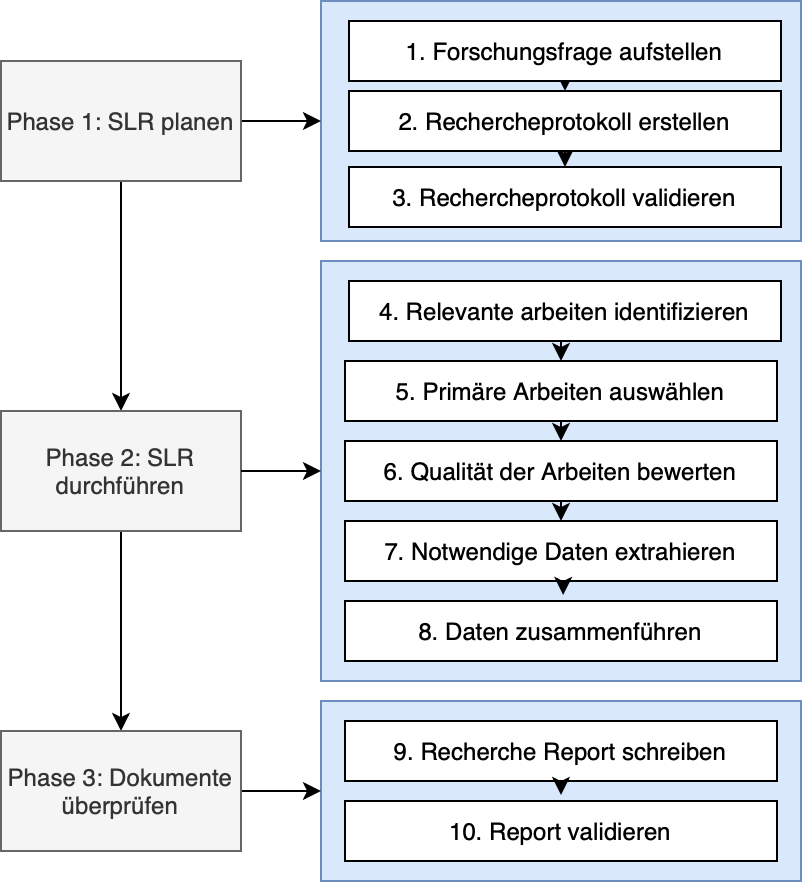
\includegraphics[width=0.8\textwidth]{graphics/slr_kitchenham_ablauf.png}
    \caption{Ablauf der systematischen Literaturrecherche nach Brereton et al. \cite{brereton2007lessons}}
    \label{fig:slr_kitchenham}
\end{figure}

\paragraph{Forschungsfrage}
Untersucht wird die Forschungsfrage: Wie können Low-Code Entwicklungsansätze 
effektiv in die Konzeption und Entwicklung von Quantencomputing-Anwendungen 
integriert werden, unter besonderer Berücksichtigung von Model-Driven 
Engineering (MDE) und Open-Source-Prinzipien?

\paragraph{Suchstrategie und Datenbanken}
In den Suchmaschinen \textit{Google Scholar}, \textit{IEEE Xplore} und \textit{ACM Digital Library} 
wird gesucht. Die Auswahl der Suchbegriffe wird strategisch vorgenommen, um die Breite und Tiefe der beiden 
Hauptthemenbereiche abzudecken. 

Die Suchbegriffe der ersten Iteration sind
\begin{itemize}
    \item \textit{Low-Code Development} 
    \item \textit{Quantum Computing}
    \item \textit{Model-Driven Engineering}
    \item \textit{Open Source}
\end{itemize} 

Um die Schnittstellen zwischen Low-Code-Plattformen und Quantencomputing genauer zu untersuchen, 
wurden die Suchbegriffe in verschiedenen Kombinationen verwendet, wobei Boolesche Operatoren wie 
AND und OR zum Einsatz kommen, um die Suche zu verfeinern und zu spezifizieren.

Die Studien müssen frühestens ab dem Jahr 2014 veröffentlicht worden sein. Dies ist insbeondere in 
Hinsicht darauf wichtig, ob das entsprechendes Tool noch aktiv gewartet wird. 
Weiterhin ist die Aktualität der Studien wichtig, da sich die Technologien und Frameworks 
im Bereich Low-Code-Entwicklung und Quantencomputing schnell weiterentwickeln.

Es werden nur Studien in englischer oder deutscher Sprache berücksichtigt, die Peer-Review-Verfahren 
durchlaufen haben. Insbesondere als relevant werden Papers erachtet, die Low-Code-Plattformen 
in Open-Source Lizensierungen behandeln. Dies vereinfacht die Verwendbarkeit für 
die spätere pilothafte Umsetzung eines Low-Code Tools für Quantencomputing-Anwendungen.

Durch die Anwendung dieser 
methodischen und strukturierten Vorgehensweise wird eine solide Basis für die Erforschung 
und Analyse der Konzeption und Entwicklung von Low-Code-Frameworks für 
Quantencomputing-Anwendungen geschaffen.

\paragraph{ResearchRabbit}
In dieser Arbeit wird ResearchRabbit als ergänzendes Tool zur systematischen Literaturrecherche eingesetzt. 
ResearchRabbit ist ein Softwaretool, das entwickelt wurde, um Arbeiten aus Forschungsgebieten als Graph darzustellen 
und relevante Verbindungen zwischen wissenschaftlichen Publikationen auf Basis von Zitierungen und thematischen 
Ähnlichkeiten zu visualisieren.\cite{cole2023researchrabbit} Nutzer des Tools geben spezifische Suchbegriffe ein, woraufhin ResearchRabbit eine 
interaktive Map generiert. Diese Maps bieten eine visuelle Darstellung, die es ermöglicht, 
zentrale Arbeiten und bisher weniger beachtete Verbindungen schnell zu identifizieren.

Die Anwendung von ResearchRabbit in der systematischen Literaturrecherche bietet erhebliche Vorteile. Erstens 
steigert das Tool die Effizienz des Rechercheprozesses, indem es durch die Visualisierung von Forschungsnetzwerken 
relevante Studien schneller erkennbar macht, was den Zeitaufwand für das erste Screening reduziert. Zweitens 
erweitert ResearchRabbit die Möglichkeit, wichtige Arbeiten zu entdecken, die in traditionellen Datenbankensuchen 
möglicherweise übersehen werden würden. Dies geschieht insbesondere durch die Aufdeckung von Querverbindungen 
zwischen verschiedenen Forschungsgebieten. Darüber hinaus ermöglicht die Analyse von Netzwerkbeziehungen 
tiefere Einblicke in die Einflussnahme und den thematischen Kontext von Schlüsselpublikationen, was zu einem 
besseren Verständnis des Forschungsstandes beiträgt. Schließlich erlaubt das Tool, aktuelle Forschungsentwicklungen 
zu verfolgen und die Literaturrecherche regelmäßig mit neuen relevanten Publikationen zu aktualisieren.

Die Entscheidung, ResearchRabbit einzusetzen, basiert auf der Notwendigkeit, eine umfangreiche und 
dynamische Forschungslandschaft effektiv zu navigieren. In sich schnell weiterentwickelnden und interdisziplinären 
Feldern wie Low-Code Development und Quantum Computing bietet ResearchRabbit einen signifikanten Mehrwert, 
indem es komplexe Informationsstrukturen zugänglich und handhabbar macht. Durch die Integration dieses Tools 
in die systematische Literaturrecherche wird nicht nur die Effizienz des Prozesses verbessert, sondern auch 
die Qualität und Tiefe der Forschungsergebnisse erhöht.

\section{Durchführung der Literaturrecherche}
Basierend auf den im vorherigen Abschnitt festgelegten Kriterien wird die systematische Literaturrecherche (SLR) 
durchgeführt. Im Folgenden werden die einzelnen Schritte der Recherche detailliert dokumentiert und die Ergebnisse 
visualisiert. Dies umfasst die spezifischen Suchanfragen in den ausgewählten wissenschaftlichen Datenbanken, die 
angewandten Suchlimits sowie die quantitativen Ergebnisse der Suchvorgänge. Durch diese detaillierte Dokumentation 
wird die Nachvollziehbarkeit und Reproduzierbarkeit der Forschung sichergestellt, während die quantitativen 
Ergebnisse eine fundierte Basis für die weitere Analyse bieten.

In der Grafik \ref{fig:search_process} ist der Ablauf der Suche nach Publikationen innerhalb der 
systematischen Literaturrecherche dargestellt. Insbesondere wird hier nochmal erwähnt, dass beim Schritt des 
Snowballings das Tool ResearchRabbit eingesetzt wird, um die Suche zu unterstützen. 

% include graphics/ablauf_der_suche.png
\begin{figure}[h!]
    \centering
    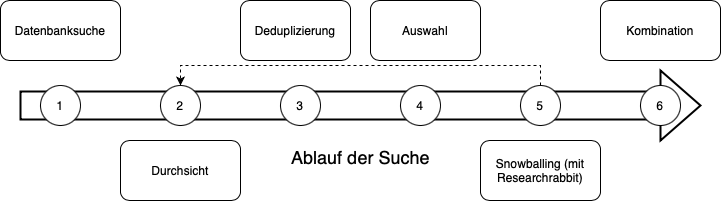
\includegraphics[width=1\textwidth]{graphics/ablauf_der_suche.png}
    \caption{Ablauf der systematischen Literaturrecherche}
    \label{fig:search_process}
\end{figure}


% \begin{itemize}
%     \item Suchprozess
%         \begin{itemize}
%             \item Durchführung der Suche in den ausgewählten Datenbanken
%                 \begin{itemize}
%                     \item Eingabe der Suchbegriffe und Kombinationen
%                     \item Anwendung von Booleschen Operatoren zur Verfeinerung
%                     \item Speichern der Suchergebnisse
%                 \end{itemize}
%             \item Dokumentation des Suchprotokolls
%                 \begin{itemize}
%                     \item Aufzeichnung der Suchbegriffe und Suchstrategien
%                     \item Festhalten der Suchergebnisse und deren Anzahl
%                     \item Datum der Suche und verwendete Datenbanken
%                 \end{itemize}
%         \end{itemize}
%     \item Screening und Auswahl der Literatur
%         \begin{itemize}
%             \item Entfernung von Duplikaten
%                 \begin{itemize}
%                     \item Identifikation und Entfernung von doppelten Einträgen
%                 \end{itemize}
%             \item Bewertung von Titeln und Abstracts
%                 \begin{itemize}
%                     \item Anwendung der Einschluss- und Ausschlusskriterien
%                     \item Erstes Screening basierend auf Titeln und Abstracts
%                     \item Dokumentation der Gründe für Ausschlüsse
%                 \end{itemize}
%             \item Volltext-Analyse
%                 \begin{itemize}
%                     \item Beschaffung der Volltexte relevanter Studien
%                     \item Detaillierte Bewertung und Anwendung der Kriterien
%                     \item Dokumentation der Gründe für endgültige Einschluss- oder Ausschlussentscheidungen
%                 \end{itemize}
%         \end{itemize}
%     \item Qualitätsbewertung der Studien
%         \begin{itemize}
%             \item Festlegung der Bewertungskriterien
%                 \begin{itemize}
%                     \item Methodische Qualität
%                     \item Validität und Verlässlichkeit der Ergebnisse
%                     \item Relevanz zur Forschungsfrage
%                 \end{itemize}
%             \item Durchführung der Qualitätsbewertung
%                 \begin{itemize}
%                     \item Anwendung der Kriterien auf die ausgewählten Studien
%                     \item Dokumentation der Bewertungsergebnisse
%                     \item Berücksichtigung der Qualität bei der Synthese der Ergebnisse
%                 \end{itemize}
%         \end{itemize}
% \end{itemize}

Um einen ersten Überblick über die Publikationen zu gewinnen wird initial die folgende Suchanfrage in den Datenbanken verwendet:

\begin{quote}
    Suchanfrage 1 (Stand: 12.07.2024):

    (''Low-Code Development'' OR ''Quantum Computing'' OR ''Model-Driven Engineering'' OR ''Open Source'')

    Erscheinungsdatum der Publikationen: 2014 - 2024
\end{quote}

\begin{table}[h!]
    \centering
    \caption{Anzahl der Suchergebnisse für Suchanfrage 1}
    \label{tab:search_1_results}
    \begin{tabular}{|l|c|}
    \hline
    \textbf{Datenbank} & \textbf{Anzahl der Ergebnisse} \\ \hline
    Google Scholar & 17.800 \\ \hline
    IEEE Xplore & 62.421 \\ \hline
    ACM Digital Library & 79.035 \\ \hline
    \end{tabular}
\end{table}
    
Diese Suchanfrage lieferte die in \ref{tab:search_1_results} dargestellten Ergebnisse. Dies 
zeigt die große Bandbreite und Relevanz der Themenfelder. 
Um hier einen Überblick zu gewinnen, wie die Verteilung der Publikationen zu den jeweiligen Konzepten ausfällt, 
wird eine Analyse der Anzahl der Publikationen pro Jahr, und Konzept, also MDE oder Low-Code vorgenommen.

Deren Ergebnisse sind in den folgenden Grafiken dargestellt:

\begin{figure}[h!]
    \centering
    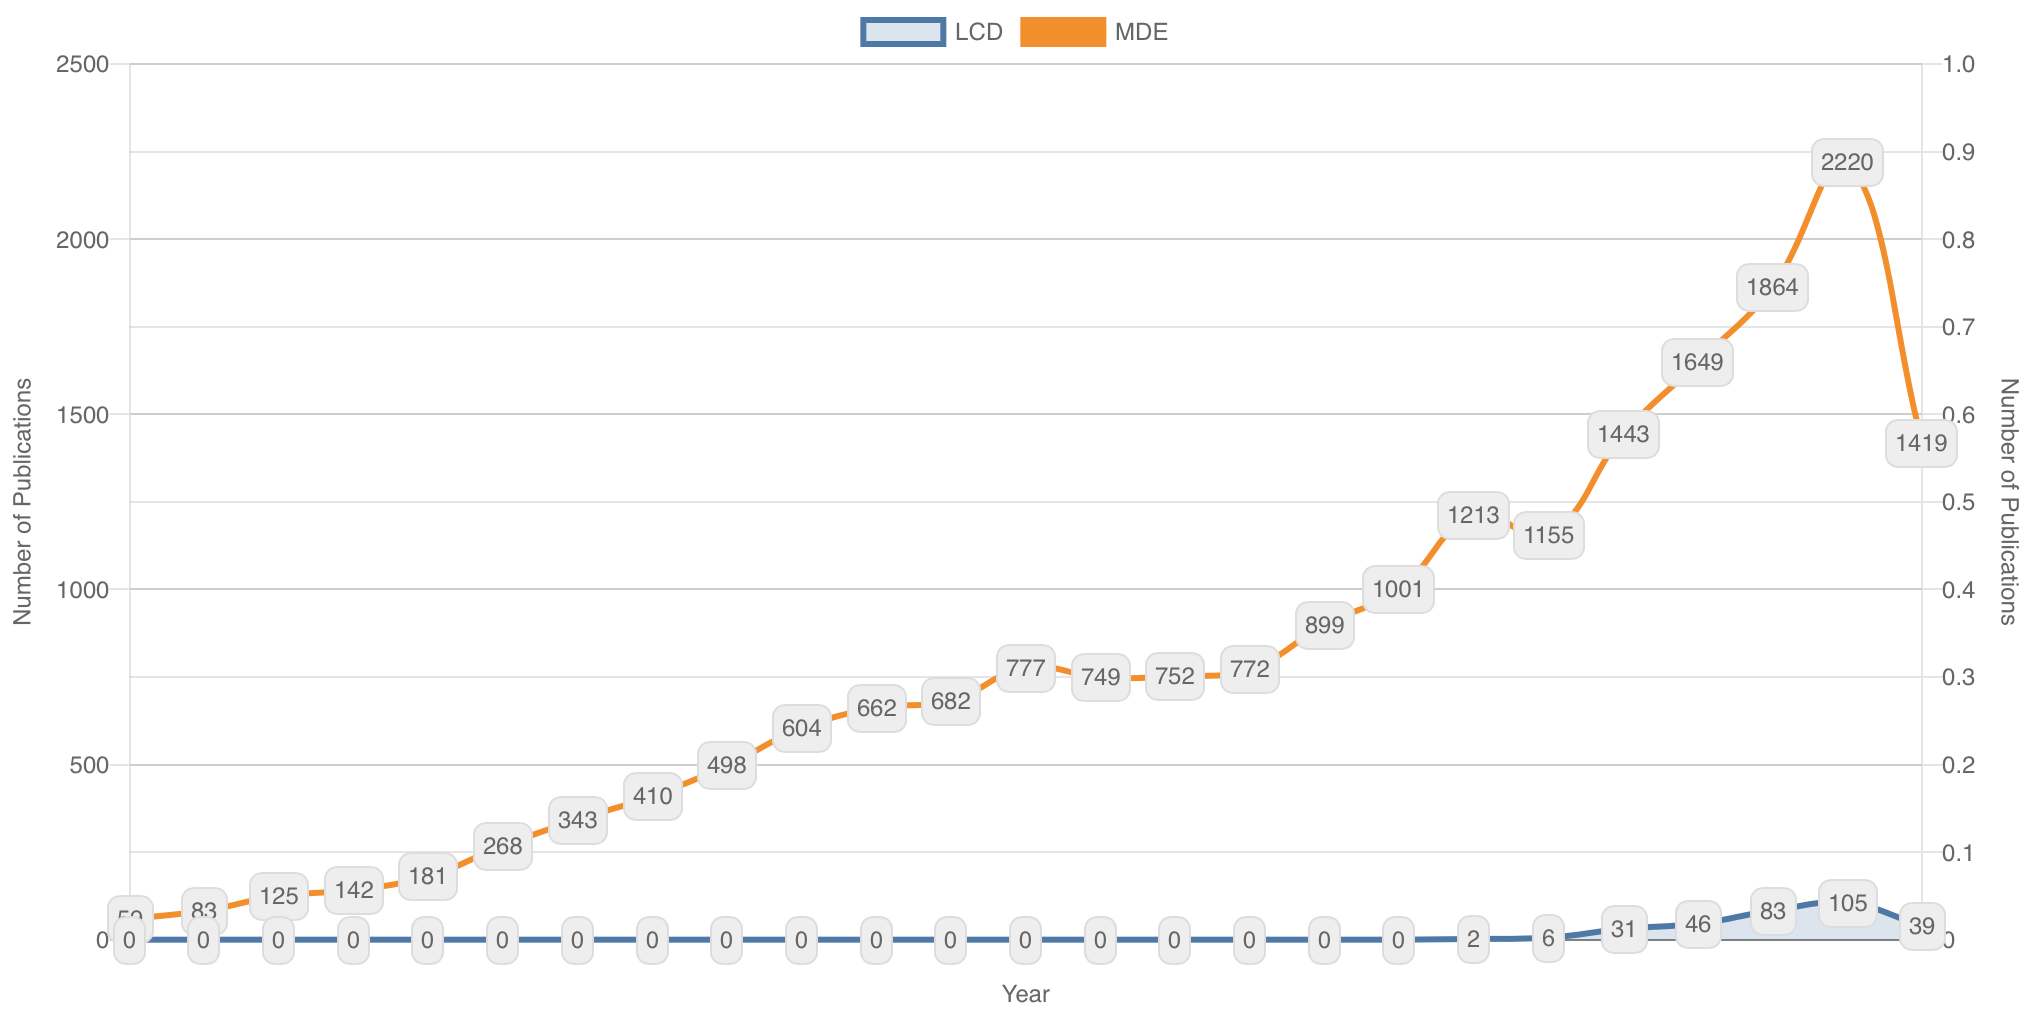
\includegraphics[width=1\textwidth]{graphics/lcd_and_mde_publications_over_years.png}
    \caption{Anzahl der Publikationen zu MDE und LCD pro Jahr}
    \label{fig:publications_mde_and_lcd_per_year}
\end{figure}

\begin{figure}[h!]
    \centering
    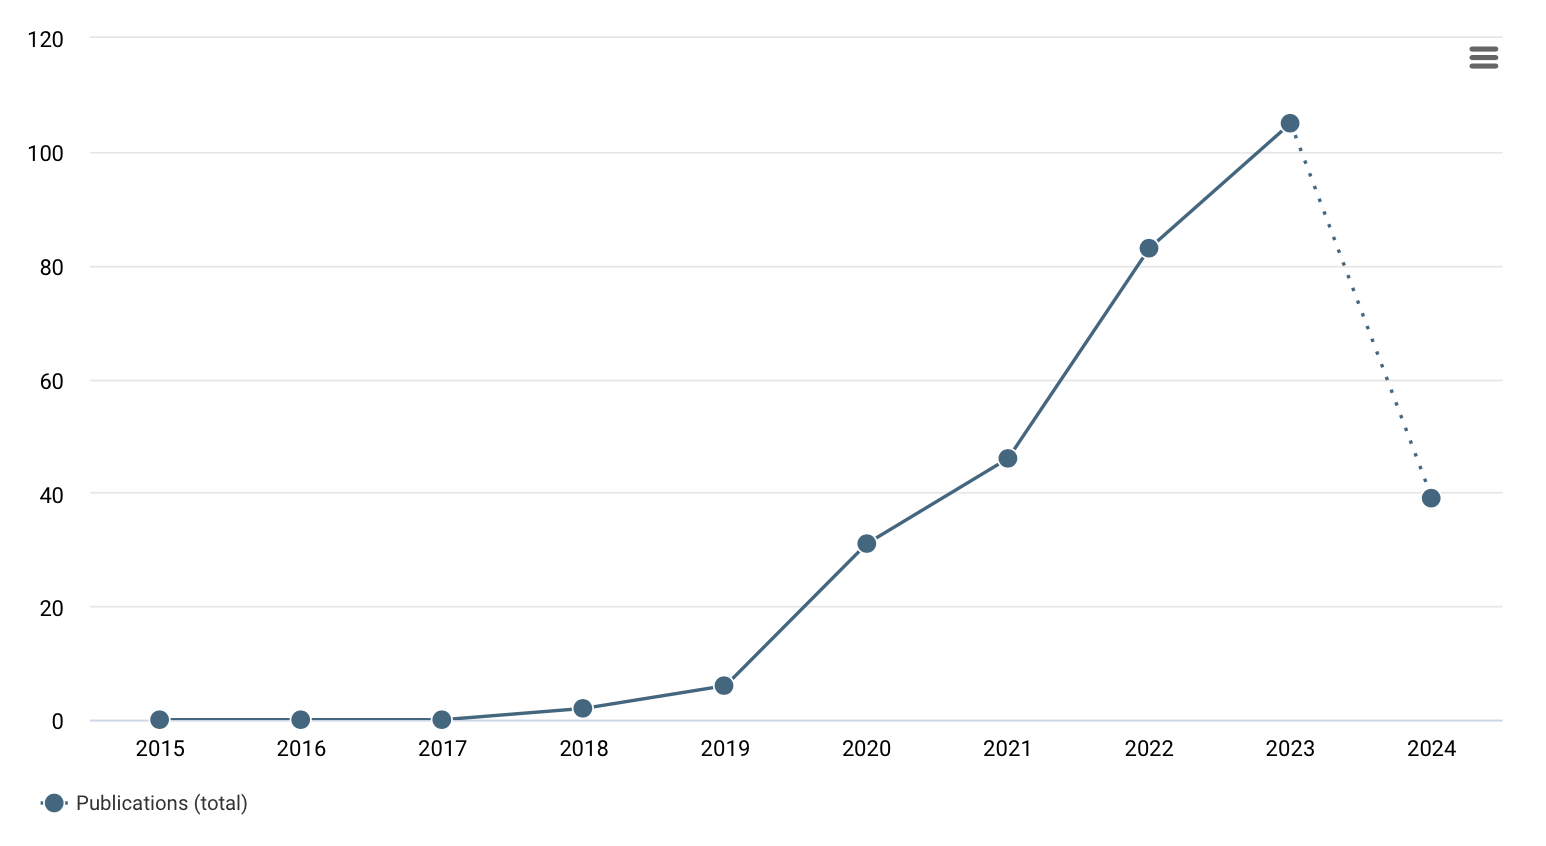
\includegraphics[width=1\textwidth]{graphics/lcd_publications_over_years.png}
    \caption{Anzahl der Publikationen LCD pro Jahr}
    \label{fig:publications_lcd_per_year}
\end{figure}

\begin{figure}[h!]
    \centering
    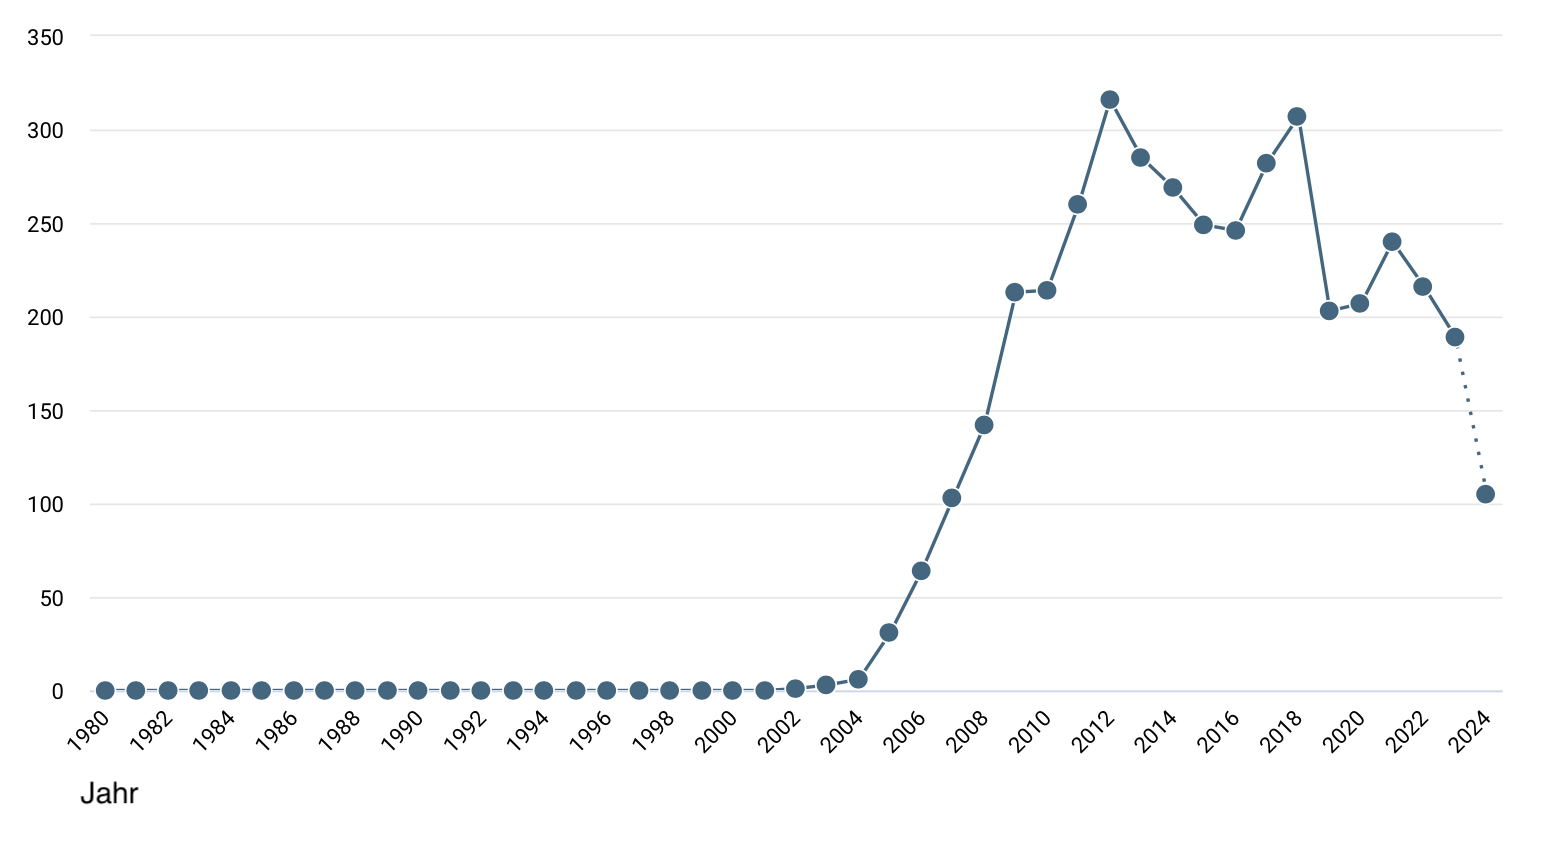
\includegraphics[width=1\textwidth]{graphics/mde_publications_over_years.png}
    \caption{Anzahl der Publikationen zu MDE pro Jahr}
    \label{fig:publications_mde_per_year}
\end{figure}

Es fällt auf, dass die Anzahl der Publikationen zu Low-Code-Entwicklung erstens insgesamt deutlich niedriger ausfällt 
als die Anzahl der Publikationen zu Model-Driven Engineering. Zweitens ist bezüglich des Erscheinungsjahres festzustellen 
das in Publikation Low-Code-Entwicklung ein deutlich jüngeres Forschungsthema ist.

Da die Anzahl der Ergebnisse zu groß ist um effektiv bearbeitet zu werden, wird die Suche 
weiter verfeinert. Weiterhin fällt beim ersten Screening auf, dass viele Ergebnisse nicht die 
gewünschte Schnittmenge aus Low-Code-Entwicklung und Quantencomputing abdecken, sondern 
nur eines der beiden Themenfelder behandeln. Um also die Relevanz der Ergebnisse zu erhöhen, 
werden spezifischere Suchanfragen formuliert. 

In einer zweiten Iteration der Suche wurde daher die folgende Suchanfrage verwendet:

\begin{quote}
    Suchanfrage 2 (Stand: 14.07.2024):

    (''Low Code Platform'' OR ''Low Code Development'' OR ''Low-Code Development'' OR ''Model-Driven Engineering'') AND (''Quantum Computing'')

    Erscheinungsdatum der Publikationen: 2014 - 2024
\end{quote}

\begin{table}[h!]
    \centering
    \caption{Anzahl der Suchergebnisse für Suchanfrage 2}
    \label{tab:search_2_results}
    \begin{tabular}{|l|c|}
    \hline
    \textbf{Datenbank} & \textbf{Anzahl der Ergebnisse} \\ \hline
    Google Scholar & 176 \\ \hline
    IEEE Xplore & 3 \\ \hline
    ACM Digital Library & 30 \\ \hline
    \end{tabular}
\end{table}

Die Ergebnisse der zweiten Suchanfrage sind in Tabelle \ref{tab:search_2_results} dargestellt. Bzgl. der Erscheinungsjahre fällt auf, dass in 
IEEE Xplore die drei Publikationen zwischen 2021 und 2023 erschienen. in der ACM Digital Library sind die Publikationen zwischen 2021 und 2024 erschienen. 
Lediglich die Google Scholar Suche ergab Publikationen, die bis ins Jahr 2014 als Untergrenze der gewünschten Filterung zurückreichen. 

Da die Anzahl der Ergebnisse nun sinnvoller ist, wird mit der Durchsicht der Titel und Abstracts fortgefahren. 
Begonnen wird mit den drei Ergebnissen aus IEEE Xplore. Durchsicht der Abstracts ergibt, dass die Publikationen 
alle drei relevant sind, da sie sich inhaltlich in der Schnittmenge aus MDE und Quantencomputing befinden. 
Um für die Datenbank IEEE Xplore den Schritt der Auswahl vorwegzugreifen, werden die drei Publikationen 
direkt in die engere Auswahl übernommen. 

Als nächsten werden die Ergebnisse der ACM Digital Library ebenfalls durchgesehen. Dabei werden beim Schritt der Auswahl notwendigerweise die 
Ergebnisse der ACM Digital Library gezielt gefiltert, um die Relevanz und Qualität der eingeschlossenen Studien sicherzustellen. 
Proceedings wurden dabei bewusst nicht in die Auswahl einbezogen. Der Grund dafür ist, dass Proceedings häufig eine 
Vielzahl von Kurzbeiträgen enthalten, die nicht denselben rigorosen Peer-Review-Prozess durchlaufen wie Journal-Artikel 
und oft eine geringere wissenschaftliche Tiefe aufweisen. Dies kann die Validität und Verlässlichkeit der 
Forschungsergebnisse beeinträchtigen. Zudem sind Proceedings meist vorläufige Ergebnisse, die 
später in detaillierteren Journal-Artikeln veröffentlicht werden. Von den initialen 30 Ergebnissen 
in der ACM Digital Library erfüllten lediglich 4 die AuswahlkriterienDurch diese Vorgehensweise wurde 
sichergestellt, dass nur qualitativ hochwertige und relevante Studien in die Analyse einbezogen wurden.

Weiterhin wurden Publikationen ausgeschlossen, deren Titel oder Abstract darauf schließen ließen, dass sie thematisch 
nicht relevant sind. Dieser Ausschluss erfolgte, um die Fokussierung auf Studien zu gewährleisten, die direkt mit 
Low-Code-Entwicklungsansätzen in Quantencomputing-Anwendungen verbunden sind. Diese strenge Selektion ist entscheidend, um 
sicherzustellen, dass die verbleibenden Studien tatsächlich die Forschungsfrage adressieren und qualitative Erkenntnisse liefern können. 

Durchsicht der 176 Ergebnisse aus Google Scholar ergab, dass 20 Publikationen die Kriterien für die engere Auswahl erfüllen. 

Für den Schritt der Deduplizierung wurden die Ergebnisse aus den drei Datenbanken zusammengeführt. 
So ergeben sich ohne Duplikate insgesamt 25 Publikationen, die für die weitere Analyse in Betracht gezogen werden. 

Bevor durch Snowballing weitere möglicherweise relevante Publikationen gesucht werden und die Volltexte der Publikationen analysiert werden, 
wird eine dritte Suchanfrage formuliert. Diese zielt darauf ab, durch eine noch feinere Fomulierung der Anfrage weitere bisher nicht gefundene 
Ergebnisse zu identifizieren. 

\begin{quote}
    Suchanfrage 3 (Stand: 16.07.2024):

    (intitle:''low-code'' quantum computing)

    Erscheinungsdatum der Publikationen: 2014 - 2024
\end{quote}

Hierfür ergibt sich die in Tabelle \ref{tab:search_3_results} dargestellte Anzahl an Ergebnissen. 

\begin{table}[h!]
    \centering
    \caption{Anzahl der Suchergebnisse für Suchanfrage 3}
    \label{tab:search_3_results}
    \begin{tabular}{|l|c|}
    \hline
    \textbf{Datenbank} & \textbf{Anzahl der Ergebnisse} \\ \hline
    Google Scholar & 26 \\ \hline
    IEEE Xplore & 1 \\ \hline
    ACM Digital Library & 8 \\ \hline
    \end{tabular}
\end{table}

Erneut ist die Anzahl an Suchergebnissen geringer geworden. Durchsicht der neuen Ergebnisse ergibt, dass zwar aus Google Scholar 
keine weiteren Publikationen in die engere Auswahl übernommen werden, jedoch aus der ACM Digital Library 7 sowie aus IEEE Xplore 1 Publikation. 
Insgesamt ergibt sich somit eine Anzahl von 33 unterschiedlichen Publikationen, die für die weitere Analyse in Betracht gezogen werden. 

Mit den nun identifizierten Publikationen wird der Schritt des Snowballings durchgeführt. Hierbei wird ResearchRabbit eingesetzt, um 
weitere Publikationen zu identifizieren, die inhaltlich mit den bereits identifizierten Publikationen in Verbindung stehen und somit 
potenziell relevant sind. Das Tool zeigt dabei die Verbindungen zwischen den Publikationen an und ermöglicht es, die Netzwerke 
zu älteren und neueren Publikationen zu visualisieren. Es ergeben sich 21 ältere Publikationen, die mit den bereits identifizierten 33 
Publikationen in Verbindung stehen. Dazu kommen 6 neuere die auf die bereits identifizierten Publikationen verweisen. 

Für diese wird nun ebenfalls der Titel und Abstract durchgesehen, um zu entscheiden, ob sie in die engere Auswahl übernommen werden. 
Insgesamt lassen sich so 13 weitere Publikationen identifizieren, die für die weitere Analyse in Betracht gezogen werden, was nun nach 
dem Schritt der Kombination zu 46 Publikationen führt. 

\section{Ergebnisse}
\begin{itemize}
    \item Übersicht der identifizierten Studien
        \begin{itemize}
            \item Anzahl der gefundenen Studien nach dem Screening
            \item Verteilung der Studien nach Jahr, Autor und Quelle
            \item Kategorisierung nach Themenbereichen (z.B. Low-Code Development, Quantum Computing, MDE, Open Source)
        \end{itemize}
    \item Synthese der Ergebnisse
        \begin{itemize}
            \item Zusammenfassung der Hauptbefunde
                \begin{itemize}
                    \item Gemeinsame Trends und Muster in den identifizierten Studien
                    \item Unterschiede und Besonderheiten in den Ansätzen
                \end{itemize}
            \item Integration der Erkenntnisse
                \begin{itemize}
                    \item Wie die Ergebnisse zur Beantwortung der Forschungsfragen beitragen
                    \item Bedeutung der Ergebnisse im Kontext der Entwicklung eines Low-Code-Frameworks für Quantencomputing
                \end{itemize}
            \item Identifikation von Forschungslücken
                \begin{itemize}
                    \item Bereiche mit wenig oder keiner Forschung
                    \item Vorschläge für zukünftige Forschungsrichtungen
                \end{itemize}
        \end{itemize}
    \item Bewertung der Ergebnisse
        \begin{itemize}
            \item Kritische Analyse der Qualität und Relevanz der gefundenen Studien
                \begin{itemize}
                    \item Stärken und Schwächen der Studien
                    \item Zuverlässigkeit und Validität der Ergebnisse
                \end{itemize}
            \item Schlussfolgerungen basierend auf der Synthese
                \begin{itemize}
                    \item Wichtige Erkenntnisse und ihre Implikationen
                    \item Empfehlungen für die Entwicklung des Low-Code-Frameworks
                \end{itemize}
        \end{itemize}
\end{itemize}

\subsection*{Anhang 1: Übersicht der Publikationen}

\setcounter{table}{0}
\renewcommand{\thetable}{A\arabic{table}}

% create a longtable to list all publications
\begin{longtable}{|m{0.8cm}|m{4.4cm}|m{3cm}|m{0.8cm}|m{4cm}|}
    \caption{Übersicht der Publikationen} 
    \label{tab:publikationen} \\
    \hline
    \textbf{ID} & \textbf{Titel} & \textbf{Autoren} & \textbf{Jahr} & \textbf{Themengebiet} \\
    \hline
    \endhead
    P01 & In Search of the Essence of Low-Code: An Exploratory Study of Seven Development Platforms & Alexander C. Bock, Ulrich Frank~\cite{Bock_2021_essence} & 2021 & Low-Code,  \\ \hline
    P02 & What about the usability in low-code platforms? A systematic literature review & Daniel Pinho et al.~\cite{Pinho_2022} & 2022 & Low-Code,  \\ \hline
    P03 & Low-Code Development Platforms - A Literature Review & Niculin Prinz et al.~\cite{Prinz_2021} & 2021 & Low-Code,  \\ \hline
    P04 & Supporting the understanding and comparison of low-code development platforms & Apurvanand Sahay et al.~\cite{Sahay_2020} & 2020 & Low-Code,  \\ \hline
    P05 & Building BESSER: an open-source low-code platform & Iván Alfonso et al.~\cite{alfonso2024building} & 2024 & Low-Code,  \\ \hline
    P06 & AI for Low-Code for AI & Nikitha Rao et al.~\cite{rao2024} & 2024 & Low-Code,  \\ \hline
    P07 & Challenges \& opportunities in low-code testing & Faezeh Khorram et al.~\cite{Khorram_2020} & 2020 & Low-Code,  \\ \hline
    P08 & Low-Code Is Often High-Code, So We Must Design Low-Code Platforms to Enable Proper Software Engineering & Timothy C. Lethbridge~\cite{lethbridge2021low} & 2021 & Low-Code,  \\ \hline
    P09 & Low-Code, No-Code, What's Under the Hood? & George Hurlburt~\cite{Hurlburt_2021} & 2021 & Low-Code,  \\ \hline
    P10 & Drivers and Inhibitors of Low Code Development Platform Adoption & Sebastian Kass et al.~\cite{Kass_2022} & 2022 & Low-Code,  \\ \hline
    P11 & A Low-Code Approach for Simulation-Based Analysis of Process Collaborations & Paolo Bocciarelli, Andrea D'Ambrogio~\cite{Bocciarelli_2023} & 2023 & Low-Code, Model-Driven Engineering,  \\ \hline
    P12 & Developer discussion topics on the adoption and barriers of low code software development platforms & Md Abdullah Al Alamin et al.~\cite{Alamin_2022} & 2022 & Low-Code, Model-Driven Engineering,  \\ \hline
    P13 & Quantumoonlight: A Low-Code Platform to Experiment with Quantum Machine Learning & Francesco Amato et al.~\cite{amato2023quantumoonlight} & 2023 & Low-Code, Quantum Computing,  \\ \hline
    P14 & Towards a Quantum Software Modeling Language & Carlos A. Pérez-Delgado et al.~\cite{Perez-Delgado_2020} & 2020 & Low-Code, Quantum Computing, Model-Driven Engineering,  \\ \hline
    P15 & Model-Driven Quantum Federated Learning (QFL) & Armin Moin et al.~\cite{Moin_2023} & 2023 & Low-Code, Quantum Computing, Model-Driven Engineering,  \\ \hline
    P16 & Towards Model-Driven Quantum Software Engineering & Felix Gemeinhardt et al.~\cite{gemeinhardt_2021} & 2021 & Low-Code, Quantum Computing, Model-Driven Engineering,  \\ \hline
    P17 & A Model-Driven Framework for Composition-Based Quantum Circuit Design & Felix Gemeinhardt et al.~\cite{Gemeinhardt_2018} & 2018 & Low-Code, Quantum Computing, Model-Driven Engineering,  \\ \hline
    P18 & A Reference Architecture for Quantum Computing as a Service & Aakash Ahmad et al.~\cite{Ahmad_2023} & 2023 & Low-Code, Quantum Computing, Model-Driven Engineering,  \\ \hline
    P19 & Design of classical-quantum systems with UML & Ricardo Pérez-Castillo et al.~\cite{perez2022design} & 2022 & Low-Code, Quantum Computing, Model-Driven Engineering,  \\ \hline
    P20 & Integrating Quantum Computing into Workflow Modeling and Execution & Benjamin Weder et al.~\cite{Weder_2020} & 2020 & Low-Code, Quantum Computing, Model-Driven Engineering,  \\ \hline
    P21 & Towards Quantum-algorithms-as-a-service & Manuel De Stefano et al.~\cite{Stefano_2022} & 2022 & Low-Code, Quantum Computing, Model-Driven Engineering,  \\ \hline
    P22 & Survey and classification of model transformation tools & Nafıseh Kahani et al.~\cite{Kahani_2019} & 2019 & Model-Driven Engineering,  \\ \hline
    P23 & Quantum Software Development with Classiq & Nir Minerbi~\cite{minerbi2022quantum} & 2022 & Quantum Computing,  \\ \hline
    P24 & Challenges of Quantum Software Engineering for the Next Decade: The Road Ahead & J. M. Murillo et al.~\cite{murillo2024challenges} & 2024 & Quantum Computing,  \\ \hline
    P25 & Software Architecture for Quantum Computing Systems - A Systematic Review & Arif  Ali Khan et al.~\cite{Khan_2022} & 2022 & Quantum Computing,  \\ \hline
    P26 & On the Definition of Quantum Programming Modules & Pedro Sánchez, Diego Alonso~\cite{Sanchez_2021} & 2021 & Quantum Computing,  \\ \hline
    P27 & Generation of Classical-Quantum Code from UML models & Ricardo Pérez-Castillo et al.~\cite{Perez-Castillo_2023} & 2023 & Quantum Computing, Model-Driven Engineering,  \\ \hline
    P28 & Model-Driven Optimization for Quantum Program Synthesis with MOMoT & Felix Gemeinhardt et al.~\cite{Gemeinhardt_2023} & 2023 & Quantum Computing, Model-Driven Engineering,  \\ \hline
    P29 & Reverse Engineering of OpenQASM3 Quantum Programs to KDM Models & Luis Jiménez-Navajas et al.~\cite{Jimenez-Navajas_2023} & 2023 & Quantum Computing, Model-Driven Engineering,  \\ \hline
    P30 & A Graph-Based Approach for Modelling Quantum Circuits & Diego Alonso et al.~\cite{alonso2023graph} & 2023 & Quantum Computing, Model-Driven Engineering,  \\ \hline
    P31 & MDE4QAI: Towards Model-Driven Engineering for Quantum Artificial Intelligence & Moin, Armin et al.~\cite{Moin_2021} & 2021 & Quantum Computing, Model-Driven Engineering,  \\ \hline
    P32 & Engineering the development of quantum programs: Application to the Boolean satisfiability problem & Diego Alonso et al.~\cite{Alonso_2022} & 2022 & Quantum Computing, Model-Driven Engineering,  \\ \hline
    P33 & Model-Driven Engineering for Quantum Programming: A Case Study on Ground State Energy Calculation & Furkan Polat et al.~\cite{polat2024model} & 2024 & Quantum Computing, Model-Driven Engineering,  \\ \hline
    P34 & Kdm to uml model transformation for quantum software modernization & Luis Jiménez-Navajas et al.~\cite{Jimenez-Navajas_2021} & 2021 & Quantum Computing, Model-Driven Engineering,  \\ \hline
    P35 & Modeling Quantum programs: challenges, initial results, and research directions & Shaukat Ali et al.~\cite{Ali_2020} & 2020 & Quantum Computing, Model-Driven Engineering,  \\ \hline
    P36 & Transforming Quantum Programs in Kdm to Quantum Design Models in Uml & Luis Jiménez-Navajas et al.~\cite{Jimenez-Navajas_2022} & 2022 & Quantum Computing, Model-Driven Engineering,  \\ \hline
    P37 & Toward a Quantum Software Engineering & Mario Piattini et al.~\cite{Piattini_2021} & 2021 & Quantum Computing, Model-Driven Engineering,  \\ \hline
    P38 & Software architecture for quantum computing systems - A systematic review & Arif Ali Khan et al.~\cite{khan2023software} & 2023 & Quantum Computing, Model-Driven Engineering,  \\ \hline
    P39 & Classical to Quantum Software Migration Journey Begins: A Conceptual Readiness Model & Muhammad Azeem Akbar et al.~\cite{Akbar_2022} & 2022 & Quantum Computing, Model-Driven Engineering,  \\ \hline
    P40 & Modelling Quantum Circuits with UML & Ricardo Pérez‐Castillo et al.~\cite{Perez-Castillo_2021} & 2021 & Quantum Computing, Model-Driven Engineering,  \\ \hline
    P41 & MDE4QAI: Towards Model-Driven Engineering for Quantum Artificial Intelligence & Armin Moin et al.~\cite{Moin_2021} & 2021 & Quantum Computing, Model-Driven Engineering,  \\ \hline
\end{longtable}




% LaTeX-Hinweise stehen in \cref{chap:latextipps}.

%noch etwas Fülltext
% \blinddocument


% \chapter{Prototypische Entwicklung des Low-Code-Frameworks für Quantencomputing}
% \label{chap:prototyp}

% \input{prototype-german.tex}


\chapter{Zusammenfassung und Ausblick}
\label{chap:zusfas}

Diese Arbeit befasste sich mit der Konzeption und Entwicklung eines Low-Code-Frameworks für Quantencomputing-Anwendungen, 
unter besonderer Berücksichtigung von Model-Driven Engineering (MDE) und Open-Source-Prinzipien. Die Motivation für diese 
Untersuchung liegt in der inhärenten Komplexität der Quantenprogrammierung, die einen hohen Einstiegspunkt für Entwickler 
darstellt, und der vielversprechenden Möglichkeit, diese Barrieren durch Low-Code-Ansätze zu senken.

Zu Beginn wurde ein umfassender Überblick über die theoretischen Grundlagen der Low-Code-Entwicklung, des Model-Driven 
Engineerings und des Quantencomputings gegeben. Dabei wurde erläutert, wie Low-Code-Entwicklungsumgebungen durch die 
Abstraktion technischer Komplexitäten und die Bereitstellung intuitiver, grafischer Entwicklungswerkzeuge die Zugänglichkeit 
zur Softwareentwicklung erhöhen können. Ebenso wurden die Potenziale und Herausforderungen von MDE in der Softwareentwicklung beschrieben.

Die systematische Literaturrecherche, die im Rahmen dieser Arbeit durchgeführt wurde, identifizierte zahlreiche Studien, 
die relevante Ansätze und Tools im Bereich Low-Code und Quantencomputing beleuchteten. Dabei wurden sowohl Gemeinsamkeiten 
als auch Unterschiede in den verschiedenen Ansätzen herausgearbeitet. Es zeigte sich, dass viele der bestehenden 
Low-Code-Entwicklungsplattformen bereits einige Aspekte der Quantenprogrammierung unterstützen, jedoch noch signifikante 
Forschungslücken bestehen.

Im Rahmen der Arbeit wurde aufgezeigt wie ein prototypisches Low-Code-Framework für Quantencomputing konzipiert werden kann, das auf den Erkenntnissen der 
Literaturrecherche basiert. 

Die Analyse der identifizierten Publikationen offenbarte zudem mehrere Forschungslücken, darunter die Notwendigkeit, robuste 
Open-Source-Tools zu entwickeln, die eine breite Anwendbarkeit und Anpassungsfähigkeit bieten. Weitere Forschung ist auch 
erforderlich, um die Effizienz und Skalierbarkeit solcher Low-Code-Frameworks im Quantencomputing-Kontext zu verbessern.

Insgesamt zeigt diese Arbeit, dass die Integration von Low-Code-Entwicklungsansätzen in die Quantencomputing-Entwicklung 
vielversprechend ist, jedoch noch in den Kinderschuhen steckt. Zukünftige Forschung sollte sich darauf konzentrieren, die 
identifizierten Lücken zu schließen und die bestehenden Frameworks weiter zu optimieren. Die Ergebnisse dieser Arbeit 
liefern wichtige Impulse und eine solide Grundlage für die Weiterentwicklung von benutzerfreundlichen, effizienten und 
zugänglichen Entwicklungswerkzeugen im Bereich des Quantencomputings.

\printbibliography

Alle URLs wurden zuletzt am 18.\,07.\,2024 geprüft.

\renewcommand{\appendixtocname}{Anhang}
\renewcommand{\appendixname}{Anhang}
\renewcommand{\appendixpagename}{Anhang}
\appendix
\appendixpage
\addappheadtotoc
\section*{Anhang}
\subsection*{Anhang 1: Übersicht der Publikationen}

\setcounter{table}{0}
\renewcommand{\thetable}{A\arabic{table}}

% create a longtable to list all publications
\begin{longtable}{|m{0.8cm}|m{4.4cm}|m{3cm}|m{0.8cm}|m{4cm}|}
    \caption{Übersicht der Publikationen} 
    \label{tab:publikationen} \\
    \hline
    \textbf{ID} & \textbf{Titel} & \textbf{Autoren} & \textbf{Jahr} & \textbf{Themengebiet} \\
    \hline
    \endhead
    P01 & In Search of the Essence of Low-Code: An Exploratory Study of Seven Development Platforms & Alexander C. Bock, Ulrich Frank~\cite{Bock_2021_essence} & 2021 & Low-Code,  \\ \hline
    P02 & What about the usability in low-code platforms? A systematic literature review & Daniel Pinho et al.~\cite{Pinho_2022} & 2022 & Low-Code,  \\ \hline
    P03 & Low-Code Development Platforms - A Literature Review & Niculin Prinz et al.~\cite{Prinz_2021} & 2021 & Low-Code,  \\ \hline
    P04 & Supporting the understanding and comparison of low-code development platforms & Apurvanand Sahay et al.~\cite{Sahay_2020} & 2020 & Low-Code,  \\ \hline
    P05 & Building BESSER: an open-source low-code platform & Iván Alfonso et al.~\cite{alfonso2024building} & 2024 & Low-Code,  \\ \hline
    P06 & AI for Low-Code for AI & Nikitha Rao et al.~\cite{rao2024} & 2024 & Low-Code,  \\ \hline
    P07 & Challenges \& opportunities in low-code testing & Faezeh Khorram et al.~\cite{Khorram_2020} & 2020 & Low-Code,  \\ \hline
    P08 & Low-Code Is Often High-Code, So We Must Design Low-Code Platforms to Enable Proper Software Engineering & Timothy C. Lethbridge~\cite{lethbridge2021low} & 2021 & Low-Code,  \\ \hline
    P09 & Low-Code, No-Code, What's Under the Hood? & George Hurlburt~\cite{Hurlburt_2021} & 2021 & Low-Code,  \\ \hline
    P10 & Drivers and Inhibitors of Low Code Development Platform Adoption & Sebastian Kass et al.~\cite{Kass_2022} & 2022 & Low-Code,  \\ \hline
    P11 & A Low-Code Approach for Simulation-Based Analysis of Process Collaborations & Paolo Bocciarelli, Andrea D'Ambrogio~\cite{Bocciarelli_2023} & 2023 & Low-Code, Model-Driven Engineering,  \\ \hline
    P12 & Developer discussion topics on the adoption and barriers of low code software development platforms & Md Abdullah Al Alamin et al.~\cite{Alamin_2022} & 2022 & Low-Code, Model-Driven Engineering,  \\ \hline
    P13 & Quantumoonlight: A Low-Code Platform to Experiment with Quantum Machine Learning & Francesco Amato et al.~\cite{amato2023quantumoonlight} & 2023 & Low-Code, Quantum Computing,  \\ \hline
    P14 & Towards a Quantum Software Modeling Language & Carlos A. Pérez-Delgado et al.~\cite{Perez-Delgado_2020} & 2020 & Low-Code, Quantum Computing, Model-Driven Engineering,  \\ \hline
    P15 & Model-Driven Quantum Federated Learning (QFL) & Armin Moin et al.~\cite{Moin_2023} & 2023 & Low-Code, Quantum Computing, Model-Driven Engineering,  \\ \hline
    P16 & Towards Model-Driven Quantum Software Engineering & Felix Gemeinhardt et al.~\cite{gemeinhardt_2021} & 2021 & Low-Code, Quantum Computing, Model-Driven Engineering,  \\ \hline
    P17 & A Model-Driven Framework for Composition-Based Quantum Circuit Design & Felix Gemeinhardt et al.~\cite{Gemeinhardt_2018} & 2018 & Low-Code, Quantum Computing, Model-Driven Engineering,  \\ \hline
    P18 & A Reference Architecture for Quantum Computing as a Service & Aakash Ahmad et al.~\cite{Ahmad_2023} & 2023 & Low-Code, Quantum Computing, Model-Driven Engineering,  \\ \hline
    P19 & Design of classical-quantum systems with UML & Ricardo Pérez-Castillo et al.~\cite{perez2022design} & 2022 & Low-Code, Quantum Computing, Model-Driven Engineering,  \\ \hline
    P20 & Integrating Quantum Computing into Workflow Modeling and Execution & Benjamin Weder et al.~\cite{Weder_2020} & 2020 & Low-Code, Quantum Computing, Model-Driven Engineering,  \\ \hline
    P21 & Towards Quantum-algorithms-as-a-service & Manuel De Stefano et al.~\cite{Stefano_2022} & 2022 & Low-Code, Quantum Computing, Model-Driven Engineering,  \\ \hline
    P22 & Survey and classification of model transformation tools & Nafıseh Kahani et al.~\cite{Kahani_2019} & 2019 & Model-Driven Engineering,  \\ \hline
    P23 & Quantum Software Development with Classiq & Nir Minerbi~\cite{minerbi2022quantum} & 2022 & Quantum Computing,  \\ \hline
    P24 & Challenges of Quantum Software Engineering for the Next Decade: The Road Ahead & J. M. Murillo et al.~\cite{murillo2024challenges} & 2024 & Quantum Computing,  \\ \hline
    P25 & Software Architecture for Quantum Computing Systems - A Systematic Review & Arif  Ali Khan et al.~\cite{Khan_2022} & 2022 & Quantum Computing,  \\ \hline
    P26 & On the Definition of Quantum Programming Modules & Pedro Sánchez, Diego Alonso~\cite{Sanchez_2021} & 2021 & Quantum Computing,  \\ \hline
    P27 & Generation of Classical-Quantum Code from UML models & Ricardo Pérez-Castillo et al.~\cite{Perez-Castillo_2023} & 2023 & Quantum Computing, Model-Driven Engineering,  \\ \hline
    P28 & Model-Driven Optimization for Quantum Program Synthesis with MOMoT & Felix Gemeinhardt et al.~\cite{Gemeinhardt_2023} & 2023 & Quantum Computing, Model-Driven Engineering,  \\ \hline
    P29 & Reverse Engineering of OpenQASM3 Quantum Programs to KDM Models & Luis Jiménez-Navajas et al.~\cite{Jimenez-Navajas_2023} & 2023 & Quantum Computing, Model-Driven Engineering,  \\ \hline
    P30 & A Graph-Based Approach for Modelling Quantum Circuits & Diego Alonso et al.~\cite{alonso2023graph} & 2023 & Quantum Computing, Model-Driven Engineering,  \\ \hline
    P31 & MDE4QAI: Towards Model-Driven Engineering for Quantum Artificial Intelligence & Moin, Armin et al.~\cite{Moin_2021} & 2021 & Quantum Computing, Model-Driven Engineering,  \\ \hline
    P32 & Engineering the development of quantum programs: Application to the Boolean satisfiability problem & Diego Alonso et al.~\cite{Alonso_2022} & 2022 & Quantum Computing, Model-Driven Engineering,  \\ \hline
    P33 & Model-Driven Engineering for Quantum Programming: A Case Study on Ground State Energy Calculation & Furkan Polat et al.~\cite{polat2024model} & 2024 & Quantum Computing, Model-Driven Engineering,  \\ \hline
    P34 & Kdm to uml model transformation for quantum software modernization & Luis Jiménez-Navajas et al.~\cite{Jimenez-Navajas_2021} & 2021 & Quantum Computing, Model-Driven Engineering,  \\ \hline
    P35 & Modeling Quantum programs: challenges, initial results, and research directions & Shaukat Ali et al.~\cite{Ali_2020} & 2020 & Quantum Computing, Model-Driven Engineering,  \\ \hline
    P36 & Transforming Quantum Programs in Kdm to Quantum Design Models in Uml & Luis Jiménez-Navajas et al.~\cite{Jimenez-Navajas_2022} & 2022 & Quantum Computing, Model-Driven Engineering,  \\ \hline
    P37 & Toward a Quantum Software Engineering & Mario Piattini et al.~\cite{Piattini_2021} & 2021 & Quantum Computing, Model-Driven Engineering,  \\ \hline
    P38 & Software architecture for quantum computing systems - A systematic review & Arif Ali Khan et al.~\cite{khan2023software} & 2023 & Quantum Computing, Model-Driven Engineering,  \\ \hline
    P39 & Classical to Quantum Software Migration Journey Begins: A Conceptual Readiness Model & Muhammad Azeem Akbar et al.~\cite{Akbar_2022} & 2022 & Quantum Computing, Model-Driven Engineering,  \\ \hline
    P40 & Modelling Quantum Circuits with UML & Ricardo Pérez‐Castillo et al.~\cite{Perez-Castillo_2021} & 2021 & Quantum Computing, Model-Driven Engineering,  \\ \hline
    P41 & MDE4QAI: Towards Model-Driven Engineering for Quantum Artificial Intelligence & Armin Moin et al.~\cite{Moin_2021} & 2021 & Quantum Computing, Model-Driven Engineering,  \\ \hline
\end{longtable}


% % !TeX root = main-german.tex
% !TeX spellcheck = de_DE
% !TeX encoding = utf8
% -*- coding:utf-8 mod:LaTeX -*-

%Die Angabe des schlauen Spruchs auf diesem Wege funtioniert nur,
%wenn keine Änderung des Kapitels mittels den in preambel/chapterheads.tex
%vorgeschlagenen Möglichkeiten durchgeführt wurde.
\setchapterpreamble[u]{%
  \dictum[Albert Einstein]{Probleme kann man niemals mit derselben Denkweise lösen, durch die sie entstanden sind.}
}
\chapter{LaTeX-Tipps}
\label{chap:latextipps}

In diesem Kapitel sollen allgemeine \LaTeX-Hinweise gegeben werden.

\section{Trennung von Absätzen}

Pro Satz eine neue Zeile.
Das ist wichtig, um sauber versionieren zu können.
In LaTeX werden Absätze durch eine Leerzeile getrennt.
Analogie zu Word: Bei Word werden neue Absätze durch einmal Eingabetaste gemacht.
Dies führt bei LaTeX jedoch nicht zu einem neuen Absatz, da LaTeX direkt aufeinanderfolgende Zeilen zu einer Zeile zusammenfügt.
Möchte man nun einen Absatz haben, muss man zweimal die Eingabetaste drücken.
Dies führt zu einer leeren Zeile.
In Word gibt es die Funktion Großschreibetaste und Eingabetaste gleichzeitig.
Wenn man dies drückt, wird einer harter Umbruch erzwungen.
Der Text fängt am Anfang der neuen Zeile an.
In LaTeX erreicht man dies durch Doppelbackslashes (\textbackslash\textbackslash) erzeugt.
Dies verwendet man quasi nie.

Folglich werden neue Abstäze insbesondere \emph{nicht} durch Doppelbackslashes erzeugt.
Beispielsweise begann der letzte Satz in einem neuen Absatz.
Eine ausführliche Motivation hierfür findet sich in \url{http://loopspace.mathforge.org/HowDidIDoThat/TeX/VCS/#section.3}.

Möchte man die Art des Absatzes ändern, so kann man die Dokumentklassenoption \texttt{parskip} verwenden.
Beispielsweise kann man mit \texttt{parskip=off} erreichen, dass statt eines freien Bereichs die erste Zeile des Absatzes eingezogen wird.

\section{File-Encoding und Unterstützung von Umlauten}
\label{sec:firstsectioninlatexhints}
Die Vorlage wurde 2010 auf UTF-8 umgestellt.
Alle neueren Editoren sollten damit keine Schwierigkeiten haben.

\section{Zitate}
Referenzen werden mittels \texttt{\textbackslash cite[key]} gesetzt.
Beispiel:~\cite{WSPA} oder mit Autorenangabe:~\citet{WSPA}.

Der folgende Satz demonstriert
\begin{filecontents*}[overwrite]{\democodefile}
\begin{inparaenum}[1.]
  \item die Großschreibung von Autorennamen am Satzanfang,
  \item die richtige Zitation unter Verwendung von Autorennamen und der Referenz,
  \item dass die Autorennamen ein Hyperlink auf das Literaturverzeichnis sind sowie
  \item dass in dem Literaturverzeichnis der Namenspräfix \qq{van der} von \qq{Wil M.\,P.\ van der Aalst} steht.
\end{inparaenum}
\end{filecontents*}

\PrintDemo{style=parallel}

\Citet{RVvdA2016} präsentieren eine Studie über die Effektivität von Workflow-Management-Systemen.

Der folgende Satz demonstriert, dass man mittels \texttt{label} in einem Bibliopgrahie"=Eintrag den Textteil des generierten Labels überschreiben kann, aber das Jahr und die Eindeutigkeit noch von biber generiert wird.
Die Apache ODE Engine~\cite{ApacheODE} ist eine Workflow-Maschine, die \BPEL-Prozesse zuverlässig ausführt.

Wörter am besten mittels \texttt{\textbackslash qq\{...\}} \qq{einschließen}, dann werden die richtigen Anführungszeichen verwendet.

Beim Erstellen der Bibtex-Datei wird empfohlen darauf zu achten, dass die DOI aufgeführt wird.

\section{Mathematische Formeln}
\label{sec:mf}
Mathematische Formeln kann man $so$ setzen. \texttt{symbols-a4.pdf} (zu finden auf \url{http://texdoc.net/pkg/symbols-a4}) enthält eine Liste der unter LaTeX direkt verfügbaren Symbole.
Beispielsweise $\mathbb{N}$ für die Menge der natürlichen Zahlen.
Für eine vollständige Dokumentation für mathematischen Formelsatz sollte die Dokumentation zu \texttt{amsmath}, \url{http://texdoc.net/pkg/amsmath} gelesen werden.

Folgende Gleichung erhält keine Nummer, da \texttt{\textbackslash equation*} verwendet wurde.
\begin{filecontents*}[overwrite]{\democodefile}
\begin{equation*}
  x = y
\end{equation*}
\end{filecontents*}

\PrintDemo{style=parallel}

Die Gleichung~\ref{eq:test} erhält eine Nummer:
\begin{filecontents*}[overwrite]{\democodefile}
\begin{equation}
  \label{eq:test}
  x = y
\end{equation}
\end{filecontents*}

\PrintDemo{style=parallel}

Die Vorlage bietet \verb+\abs+ an, damit die Absolutbetragsstriche richtig skalieren:
$\abs{X}$.

Eine ausführliche Anleitung zum Mathematikmodus von LaTeX findet sich in \url{http://www.ctan.org/tex-archive/help/Catalogue/entries/voss-mathmode.html}.

\section{Quellcode}
\Cref{lst:ListingANDlstlisting,helloworld} zeigen, wie man Programmlistings einbindet.
Mittels \texttt{\textbackslash lstinputlisting} kann man den Inhalt direkt aus Dateien lesen.

%Listing-Umgebung wurde durch \newfloat{Listing} definiert

\begin{Listing}
  \begin{lstlisting}[language=XML]
<listing name="second sample">
  <!-- comment -->
  <content>not interesting</content>
</listing>
\end{lstlisting}
  \caption{lstlisting in einer Listings-Umgebung, damit das Listing durch Balken abgetrennt ist}
  \label{lst:ListingANDlstlisting}
\end{Listing}


%TODO: Currently not shown in TOC
\lstinputlisting[language=C++,label=helloworld,caption={"`hello world"' in C++.},float]{code/helloworld.cpp}

Quellcode im \lstinline|<listing />| ist auch möglich.


\section{Pseudocode}
\Cref{alg:sample} zeigt einen Beispielalgorithmus.


\begin{Algorithmus} %Die Umgebung nur benutzen, wenn man den Algorithmus ähnlich wie Graphiken von TeX platzieren lassen möchte
  \caption{Sample algorithm}
  \label{alg:sample}
  %EN: This is an environment from the algorithmicx package
  \begin{algorithmic}
    \Procedure{Sample}{$a$,$v_e$}
      \State $\mathsf{parentHandled} \gets (a = \mathsf{process}) \lor \mathsf{visited}(a'), (a',c,a) \in \mathsf{HR}$
      \State \Comment $(a',c'a) \in \mathsf{HR}$ denotes that $a'$ is the parent of $a$
    \If{$\mathsf{parentHandled}\,\land(\mathcal{L}_\mathit{in}(a)=\emptyset\,\lor\,\forall l \in \mathcal{L}_\mathit{in}(a): \mathsf{visited}(l))$}
      \State $\mathsf{visited}(a) \gets \text{true}$
      \State $\mathsf{writes}_\circ(a,v_e) \gets
        \begin{cases}
          \mathsf{joinLinks}(a,v_e)                & \abs{\mathcal{L}_\mathit{in}(a)} > 0 \\
          \mathsf{writes}_\circ(p,v_e)
                                                   & \exists p: (p,c,a) \in \mathsf{HR}   \\
          (\emptyset, \emptyset, \emptyset, false) & \text{otherwise}
        \end{cases}
      $
    \If{$a\in\mathcal{A}_\mathit{basic}$}
      \State \Call{HandleBasicActivity}{$a$,$v_e$}
    \ElsIf{$a\in\mathcal{A}_\mathit{flow}$}
      \State \Call{HandleFlow}{$a$,$v_e$}
    \ElsIf{$a = \mathsf{process}$} \Comment Directly handle the contained activity
      \State \Call{HandleActivity}{$a'$,$v_e$}, $(a,\bot,a') \in \mathsf{HR}$
      \State $\mathsf{writes}_\bullet(a) \gets \mathsf{writes}_\bullet(a')$
    \EndIf
    \ForAll{$l \in \mathcal{L}_\mathit{out}(a)$}
      \State \Call{HandleLink}{$l$,$v_e$}
    \EndFor
    \EndIf
    \EndProcedure
  \end{algorithmic}
\end{Algorithmus}

\clearpage
Und wer einen Algorithmus schreiben möchte, der über mehrere Seiten geht, der kann das nur mit folgendem \textbf{üblen} Hack tun:

{
\begin{minipage}{\textwidth}
  \hrule height .8pt width\textwidth
  \vskip.3em%\vskip\abovecaptionskip\relax
  \stepcounter{Algorithmus}
  \addcontentsline{alg}{Algorithmus}{\protect\numberline{\theAlgorithmus}{\ignorespaces Description \relax}}
  \noindent\textbf{Algorithmus \theAlgorithmus} Description
  %\stepcounter{algorithm}
  %\addcontentsline{alg}{Algorithmus}{\thealgorithm{}\hskip0em Description}
  %\textbf{Algorithmus \thealgorithm} Description
  \vskip.3em%\vskip\belowcaptionskip\relax
  \hrule height .5pt width\textwidth
\end{minipage}
%without the following line, the text is never at the rule
\vskip-.3em
%
code goes here\\
test2\\
%
\vskip-.7em
\hrule height .5pt width\textwidth
}




\section{Abbildungen}

Die \cref{fig:chor1} und~\ref{fig:chor2} sind für das Verständnis dieses Dokuments wichtig.
Im Anhang zeigt \vref{fig:AnhangsChor} erneut die komplette Choreographie.

%Die Parameter in eckigen Klammern sind optionale Parameter - z.B. [htb!]
%htb! bedeutet: "Liebes LaTeX, bitte platziere diese Abbildung zuerst hier ("_h_ere"). Falls das nicht funktioniert, dann bitte oben auf der Seite ("_t_op"). Und falls das nicht geht, bitte unten auf der Seite ("_b_ottom"). Und bitte, bitte bevorzuge hier und oben, auch wenn's net so optimal aussieht ("!")
%Diese sollten nach Möglichkeit NICHT verwendet werden. LaTeX's Algorithmus für das Platzieren der Gleitumgebung ist schon sehr gut!

\begin{figure}
  \centering
  \includegraphics[width=\textwidth]{choreography.pdf}
  \caption{Beispiel-Choreographie}
  \label{fig:chor1}
\end{figure}



\begin{figure}
  \centering
  \includegraphics[width=.8\textwidth]{choreography.pdf}
  \caption[Beispiel-Choreographie]{Die Beispiel-Choreographie.
    Nun etwas kleiner, damit \texttt{\textbackslash textwidth} demonstriert wird.
    Und auch die Verwendung von alternativen Bildunterschriften für das Verzeichnis der Abbildungen.
    Letzteres ist allerdings nur Bedingt zu empfehlen, denn wer liest schon so viel Text unter einem Bild?
    Oder ist es einfach nur Stilsache?
  }
  \label{fig:chor2}
\end{figure}


\begin{figure}
  \hfill
  \begin{subfigure}{.3\textwidth}
    \includegraphics[width=\textwidth]{choreography.pdf}
    \caption{Choreografie 1}
    \label{fig:subfigA}
  \end{subfigure}
  \hfill
  \begin{subfigure}{.3\textwidth}
    \includegraphics[width=\textwidth]{choreography.pdf}
    \caption{Choreografie 2}
    \label{fig:subfigB}
  \end{subfigure}
  \hfill
  \begin{subfigure}{.3\textwidth}
    \includegraphics[width=.9\textwidth]{choreography.pdf}
    \caption{Choreografie 3}
    \label{fig:subfigC}
  \end{subfigure}
  \caption{Beispiel um 3 Abbildung nebeneinader zu stellen nur jedes einzeln referenzieren zu können.}
  \label{fig:subfig_example}
\end{figure}

\Cref{fig:subfig_example} zeigt die Verwendung des subcaption-Pakets.
Es ist auch möglich, auf Unterabbildungen zu verweisen: \Cref{fig:subfigA}.

Es ist möglich, SVGs direkt beim Kompilieren in PDF umzuwandeln.
Dies ist im Quellcode zu latex-tipps.tex beschrieben, allerdings auskommentiert.

\iffalse % <-- Das hier wegnehmen, falls inkscape im Pfad ist
  Das SVG in \cref{fig:directSVG} ist direkt eingebunden, während der Text im SVG in \cref{fig:latexSVG} mittels pdflatex gesetzt ist.
  Falls man die Graphiken sehen möchte, muss inkscape im PATH sein und im Tex-Quelltext \texttt{\textbackslash{}iffalse} und \texttt{\textbackslash{}iftrue} auskommentiert sein.

  \begin{figure}
    \centering
    \includegraphics{svgexample.svg}
    \caption{SVG direkt eingebunden}
    \label{fig:directSVG}
  \end{figure}

  \begin{figure}
    \centering
    \def\svgwidth{.4\textwidth}
    \includesvg{svgexample}
    \caption{Text im SVG mittels \LaTeX{} gesetzt}
    \label{fig:latexSVG}
  \end{figure}
\fi % <-- Das hier wegnehmen, falls inkscape im Pfad ist


\section{Weitere Illustrationen}
\Cref{fig:AnhangsChor,fig:AnhangsChor2} zeigen zwei Choreographien, die den Sachverhalt weiter erläutern sollen.
Die zweite Abbildung ist um 90 Grad gedreht, um das Paket \texttt{pdflscape} zu demonstrieren.

\begin{figure}
  \centering
  \includegraphics[width=\textwidth]{choreography.pdf}
  \caption{Beispiel-Choreographie I}
  \label{fig:AnhangsChor}
\end{figure}

\begin{landscape}
  \begin{figure}
    \centering
    \includegraphics[width=\textwidth]{choreography.pdf}
    \caption{Beispiel-Choreographie II}
    \label{fig:AnhangsChor2}
  \end{figure}
\end{landscape}


\iffalse

  \clearpage

  FIXME - This does not work with MiKTeX as of 2016-12-30

  TODO- demonstrate rotating package

  %hint by http://tex.stackexchange.com/a/3265/9075
  %other option is to use changepage according to http://tex.stackexchange.com/a/2639/9075. This, however, has issues with landscape
  \thispagestyle{empty}

  \savegeometry{koma}

  %If you only have height problems, this is not needed at all
  \addtolength{\textwidth}{2cm}
  \addtolength{\evensidemargin}{-1cm}

  \begin{landscape}
    %sidewaysfigure
    \begin{figure}
      \centering
      \includegraphics[width=0.9\paperheight]{choreography.pdf}
      \caption{Beispiel-Choreographie, auf einer weißen Seite gezeigt wird und über die definierten Seitenränder herausragt}
    \end{figure}
  \end{landscape}

  %the original layout is restored.
  %%\restoregeometry cannot be used as we use \addtolength
  \loadgeometry{koma}

\fi

\IfFileExists{pgfplots.sty}{
  \section{Plots with pgfplots}
  Pgfplot ist ein Paket um Graphen zu plotten ohne den Umweg über gnuplot oder matplotlib zu gehen.
  %hint by http://tex.stackexchange.com/a/3265/9075%other option is to use changepage according to http://tex.stackexchange.com/a/2639/9075. This, however, has issues with landscape%If you only have height problems, this is not needed at all%sidewaysfigure%the original layout is restored.%%\restoregeometry cannot be used as we use \addtolength
  \begin{figure}[h]
    \centering
    \begin{tikzpicture}
      \begin{axis}[xlabel=$x$,
          ylabel=$\sin(x)$]
        \addplot {sin(deg(x))};  % Sinus-Funktion zeichnen
      \end{axis}
    \end{tikzpicture}
    \caption{$\sin(x)$ mit pgfplots.}
  \end{figure}

   \begin{figure}[h]
    \centering
    \begin{tikzpicture}
      \begin{axis}[xlabel=$x$,
          ylabel=$y$]
        \addplot table [x=a, y=c, col sep=comma] {data/data.csv};  % Koordinaten aus einer CSV-Datei lesen und plotten
      \end{axis}
    \end{tikzpicture}
    \caption{Koordianten $x$ und $y$ aus einer CSV-Datei geplottet mit pgfplots.}
  \end{figure}

}{}

\section{Figures with tikz}
TikZ ist ein Paket um Zeichnungen mittels Programmierung zu erstellen.
Dieses Paket eignet sich um Gitter zu erstellen oder andere regelmäßige Strukturen zu erstellen.
Hier gibt es sehr viele visuelle Beispiele was tikz alles kann\footnote{\url{http://texdoc.net/pkg/visualtikz}}.

\begin{figure}[ht]
  \centering
  \begin{tikzpicture}
    \draw(0,0) rectangle (4,4);
    \foreach \x in {0.5,1,1.5,2,2.5,3,3.5}
    \foreach \y in {0.5,1,1.5,2,2.5,3,3.5}
    \draw(\x,\y) circle (1pt);
  \end{tikzpicture}
  \caption{Eine tikz-Graphik.}\label{fig:tikz_example}
\end{figure}


\section{UML-Diagramme mit tikz-uml}

\Cref{fig:uml} zeigt ein Klassendiagramm, das mittels tikz-uml gesetzt wurde.

\begin{figure}
  \centering
  \begin{tikzpicture}
  \begin{umlpackage}{p}
  \begin{umlpackage}{sp1}
  \umlclass[template=T]{A}{
    n : uint \\ t : float
  }{}
  \umlclass[y=-3]{B}{
    d : double
  }{
    \umlvirt{setB(b : B) : void} \\ getB() : B}
  \end{umlpackage}
  \begin{umlpackage}[x=10,y=-6]{sp2}
  \umlinterface{C}{
    n : uint \\ s : string
  }{}
  \end{umlpackage}
  \umlclass[x=2,y=-10]{D}{
    n : uint
    }{}
  \end{umlpackage}

  \umlassoc[geometry=-|-, arg1=tata, mult1=*, pos1=0.3, arg2=toto, mult2=1, pos2=2.9, align2=left]{C}{B}
  \umlunicompo[geometry=-|, arg=titi, mult=*, pos=1.7, stereo=vector]{D}{C}
  \umlimport[geometry=|-, anchors=90 and 50, name=import]{sp2}{sp1}
  \umlaggreg[arg=tutu, mult=1, pos=0.8, angle1=30, angle2=60, loopsize=2cm]{D}{D}
  \umlinherit[geometry=-|]{D}{B}
  \umlnote[x=2.5,y=-6, width=3cm]{B}{Eine Notiz f\"ur die Klasse B}
  \umlnote[x=7.5,y=-2]{import-2}{Eine Anmerkung}
  \end{tikzpicture}
  \caption{Ein Klassendiagramm mit tikz-uml generiert. Beispiel von Nicolas Kielbasiewicz adaptiert.}
  \label{fig:uml}
\end{figure}

\section{Tabellen}

\cref{tab:Ergebnisse} zeigt Ergebnisse und die \cref{tab:Ergebnisse} zeigt wie numerische Daten in einer Tabelle representiert werden können.
\begin{table}
  \centering
  \begin{tabular}{ccc}
    \toprule
    \multicolumn{2}{c}{\textbf{zusammengefasst}} & \textbf{Titel}                                                          \\ \midrule
    Tabelle                                      & wie                                                           & in      \\
    \url{tabsatz.pdf}                            & empfohlen                                                     & gesetzt \\

    \multirow{2}{*}{Beispiel}                    & \multicolumn{2}{c}{ein schönes Beispiel}                                \\
                                                 & \multicolumn{2}{c}{für die Verwendung von \qq{multirow}}           \\
    \bottomrule
  \end{tabular}
  \caption[Beispieltabelle]{Beispieltabelle -- siehe \url{http://www.ctan.org/tex-archive/info/german/tabsatz/}}
  \label{tab:Ergebnisse}
\end{table}

\begin{table}
  \centering
  \begin{tabular}{l *{8}{d{3.2}}}
    \toprule

                         & \multicolumn{2}{c}{\textbf{Parameter 1}} & \multicolumn{2}{c}{\textbf{Parameter 2}} & \multicolumn{2}{c}{\textbf{Parameter 3}} & \multicolumn{2}{c}{\textbf{Parameter 4}}                                                                                                                                       \\
    \cmidrule(r){2-3}\cmidrule(lr){4-5}\cmidrule(lr){6-7}\cmidrule(l){8-9}

    \textbf{Bedingungen} & \multicolumn{1}{c}{\textbf{M}}           & \multicolumn{1}{c}{\textbf{SD}}          & \multicolumn{1}{c}{\textbf{M}}           & \multicolumn{1}{c}{\textbf{SD}}          & \multicolumn{1}{c}{\textbf{M}} & \multicolumn{1}{c}{\textbf{SD}} & \multicolumn{1}{c}{\textbf{M}} & \multicolumn{1}{c}{\textbf{SD}} \\
    \midrule

    W                    & 1.1                                      & 5.55                                     & 6.66                                     & .01                                      &                                &                                 &                                &                                 \\
    X                    & 22.22                                    & 0.0                                      & 77.5                                     & .1                                       &                                &                                 &                                &                                 \\
    Y                    & 333.3                                    & .1                                       & 11.11                                    & .05                                      &                                &                                 &                                &                                 \\
    Z                    & 4444.44                                  & 77.77                                    & 14.06                                    & .3                                       &                                &                                 &                                &                                 \\
    \bottomrule
  \end{tabular}

  \caption{
    Beispieltabelle f\"{u}r 4 Bedingungen (W-Z) mit jeweils 4 Parameters mit (M und SD).
    Hinweis: Stets die selbe Anzahl an Nachkommastellen angeben.
  }
  \label{tab:Werte}
\end{table}



\IfFileExists{pgfplotstable.sty}{

\subsection{Tabellen mit pgfplots}
Mit pgfplots koennen Tabellen direkt aus einer CSV-Datei erstellt werden.

\begin{table}[h]
\centering
\pgfplotstabletypeset[
col sep = comma,
every head row/.style={before row=\toprule,after row=\midrule},
every last row/.style={after row=\bottomrule},
display columns/0/.style={string type,column name={}}
]
{data/data.csv}
\caption{Tabelle generiert aus einer CSV-Datei mit pgfplots}
\end{table}
}{}


\section{Tabellen über mehere Seiten}

\begin{longtable}{|l|l|l|}
\caption{Tabelle \"uber mehere Seiten} \label{tab:long} \\

\hline \multicolumn{1}{|c|}{\textbf{A}} & \multicolumn{1}{c|}{\textbf{B}} & \multicolumn{1}{c|}{\textbf{B}} \\ \hline
\endfirsthead

\multicolumn{3}{c}%
{{\bfseries \tablename\ \thetable{} -- von dor vorherigen Seite weitergeführt}} \\
\hline \multicolumn{1}{|c|}{\textbf{First column}} & \multicolumn{1}{c|}{\textbf{Second column}} & \multicolumn{1}{c|}{\textbf{Third column}} \\ \hline
\endhead

\hline \multicolumn{3}{|r|}{{Wird auf der n\"achsten Seite fortgef\"uhrt}} \\ \hline
\endfoot

\hline \hline
\endlastfoot

A & B C & D \\
A & B C & D \\
A & B C & D \\
A & B C & D \\
A & B C & D \\
A & B C & D \\
A & B C & D \\
A & B C & D \\
A & B C & D \\
A & B C & D \\
A & B C & D \\
A & B C & D \\
A & B C & D \\
A & B C & D \\
A & B C & D \\
A & B C & D \\
A & B C & D \\
A & B C & D \\
A & B C & D \\
A & B C & D \\
A & B C & D \\
A & B C & D \\
A & B C & D \\
A & B C & D \\
A & B C & D \\
A & B C & D \\
A & B C & D \\
A & B C & D \\
A & B C & D \\
A & B C & D \\
A & B C & D \\
A & B C & D \\
A & B C & D \\
A & B C & D \\
A & B C & D \\
A & B C & D \\
A & B C & D \\
A & B C & D \\
A & B C & D \\
A & B C & D \\
A & B C & D \\
A & B C & D \\
A & B C & D \\
A & B C & D \\
A & B C & D \\
A & B C & D \\
A & B C & D \\
A & B C & D \\
A & B C & D \\
A & B C & D \\
A & B C & D \\
A & B C & D \\
A & B C & D \\
A & B C & D \\
A & B C & D \\
A & B C & D \\
A & B C & D \\
A & B C & D \\
A & B C & D \\
A & B C & D \\
A & B C & D \\
A & B C & D \\
A & B C & D \\
A & B C & D \\
A & B C & D \\
A & B C & D \\
A & B C & D \\
A & B C & D \\
A & B C & D \\
A & B C & D \\
A & B C & D \\
A & B C & D \\
A & B C & D \\
A & B C & D \\
A & B C & D \\
A & B C & D \\
A & B C & D \\
A & B C & D \\
A & B C & D \\
A & B C & D \\
\end{longtable}


\section{Abkürzungen}

Beim ersten Durchlauf betrug die \gls{fr} 5.
Beim zweiten Durchlauf war die \gls{fr} 3.
Die Pluralform sieht man hier: \glspl{er}.
Um zu demonstrieren, wie das Abkürzungsverzeichnis bei längeren Beschreibungstexten aussieht, muss hier noch \glspl{rdbms} erwähnt werden.

Mit \verb+\gls{...}+ können Abkürzungen eingebaut werden, beim ersten Aufrufen wird die lange Form eingesetzt.
Beim wiederholten Verwenden von \verb+\gls{...}+ wird automatisch die kurz Form angezeigt.
Außerdem wird die Abkürzung automatisch in die Abkürzungsliste eingefügt.
Mit \verb+\glspl{...}+ wird die Pluralform verwendet.
Möchte man, dass bei der ersten Verwendung direkt die Kurzform erscheint, so kann man mit \verb+\glsunset{...}+ eine Abkürzung als bereits verwendet markieren.
Das Gegenteil erreicht man mit \verb+\glsreset{...}+.

Definiert werden Abkürzungen in der Datei \textit{content\\ausarbeitung.tex} mithilfe von \verb+\newacronym{...}{...}{...}+.

Mehr Infos unter: \url{http://tug.ctan.org/macros/latex/contrib/glossaries/glossariesbegin.pdf}


\section{Verweise}
Für weit entfernte Abschnitte ist \qq{varioref} zu empfehlen:
\qq{Siehe \vref{sec:mf}}.
Das Kommando \texttt{\textbackslash{}vref} funktioniert ähnlich wie \texttt{\textbackslash{}cref} mit dem Unterschied, dass zusätzlich ein Verweis auf die Seite hinzugefügt wird.
\texttt{vref}: \qq{\vref{sec:firstsectioninlatexhints}}, \texttt{cref}: \qq{\cref{sec:firstsectioninlatexhints}}, \texttt{ref}: \qq{\ref{sec:firstsectioninlatexhints}}.

Falls \qq{varioref} Schwierigkeiten macht, dann kann man stattdessen \qq{cref} verwenden.
Dies erzeugt auch das Wort \qq{Abschnitt} automatisch: \cref{sec:mf}.
Das geht auch für Abbildungen usw.
Im Englischen bitte \verb1\Cref{...}1 (mit großem \qq{C} am Anfang) verwenden.


%Mit MiKTeX Installation ab dem 2012-01-16 nicht mehr nötig
%Falls ein Abschnitt länger als eine Seite wird und man mittels \texttt{\textbackslash{}vref} auf eine konkrete Stelle in der Section
%verweisen möchte, dann sollte man \texttt{\textbackslash{}phantomsection} verwenden und dann wird
%auch bei \texttt{vref} die richtige Seite angeben.

%%The link location will be placed on the line below.
%%Tipp von http://en.wikibooks.org/wiki/LaTeX/Labels_and_Cross-referencing#The_hyperref_package_and_.5Cphantomsection
%\phantomsection
%\label{alabel}
%Das Beispiel für \texttt{\textbackslash{}phantomsection} bitte im \LaTeX{}-Quellcode anschauen.

%Hier das Beispiel: Siehe Abschnitt \vref{hack1} und Abschnitt \vref{hack2}.


\section{Definitionen}
\begin{definition}[Title]
  \label{def:def1}
  Definition Text
\end{definition}

\Cref{def:def1} zeigt \ldots

\section{Fußnoten}
Fußnoten können mit dem Befehl \verb+\footnote{...}+ gesetzt werden\footnote{\label{fussnote}Diese Fußnote ist ein Beispiel.
}.
Mehrfache Verwendung von Fußnoten ist möglich indem man zu erst ein Label in der Fußnote setzt \verb+\footnote{\label{...}...}+ und anschließend mittels \verb+\cref{...}+ die Fußnote erneut verwendet\cref{fussnote}.


\section{Verschiedenes}
\label{sec:diff}
\ifdeutsch
  Ziffern (123\,654\,789) werden schön gesetzt.
  Entweder in einer Linie oder als Minuskel-Ziffern.
  Letzteres erreicht man durch den Parameter \texttt{osf} bei dem Paket \texttt{libertine} bzw.\ \texttt{mathpazo} in \texttt{fonts.tex}.
\fi

\begin{compactenum}[I.]
  \item Man kann auch die Nummerierung dank paralist kompakt halten
  \item und auf eine andere Nummerierung umstellen
\end{compactenum}

Die Wörter \qq{Workflow} und \qq{Auflage} lassen sich im PDF kopieren und in eine Textdatei einfügen.

Bei der Nutzung von \LuaLaTeX{} wird bei \qq{Auflage} automatisch keine Ligatur bei \qq{f\/l} (im Gegensatz zu \qq{fl} bei \qq{workflow}) gesetzt.
In anderen Worten: \qq{Auflage} und \qq{Auf\/lage} sehen im Falle der Nutzung von \LuaLaTeX{} im PDF gleich aus.
Weiterhin setzt dieses Vorgehen die Duden-Regeln bezüglich \qq{Ligaturen}~\cite[S.\ 96]{Duden2001} um.

\section{Schlusswort}
Verbesserungsvorschläge für diese Vorlage sind immer willkommen.
Bitte bei GitHub ein Ticket eintragen (\url{https://github.com/latextemplates/scientific-thesis-template/issues}).


\pagestyle{empty}
\renewcommand*{\chapterpagestyle}{empty}
\Versicherung
\end{document}
